\documentclass[12pt,a4paper,openany,oneside]{book}

%------------------------------------------------------------------------------%
%                                                                              %
%   LaTeX Template for Bachlor Thesis of Northwestern Polytechnical University %
%   Using XeLeTeX + MakeIndex + BibTeX, or Using CTeX v2.9.2.164               %
%   Version: 1.0.0                                                             %
%                                                                              %
%------------------------------------------------------------------------------%
%   Copyright 2016 by Shangkun Shen, MIT-LICENSE(see mit-license.polossk.com)  %
%------------------------------------------------------------------------------%


%---------------------------------纸张大小设置---------------------------------%
\usepackage{geometry}
    % 普通A4格式缩进
    % \geometry{left=2.5cm,right=2.5cm,top=2.5cm,bottom=2.5cm}
    % 论文标准缩进
    \geometry{left=1.25in,right=1.25in,top=1in,bottom=1.5in}
%------------------------------------------------------------------------------%


%----------------------------------必要库支持----------------------------------%
\usepackage{amsmath}
\usepackage{amssymb}
\usepackage{amsfonts}
\usepackage{mathrsfs}
\usepackage{bm}
\usepackage{xcolor}
\usepackage{tikz}
\usepackage{layouts}
\usepackage[numbers,sort&compress]{natbib}
\usepackage{clrscode}

\usepackage{dirtree}
\usepackage{url}
%------------------------------------------------------------------------------%


%--------------------------------设置标题与目录--------------------------------%
\usepackage[sf]{titlesec}
\usepackage{titletoc}
%------------------------------------------------------------------------------%


%--------------------------------添加书签超链接--------------------------------%
\usepackage[unicode=true,colorlinks=false,pdfborder={0 0 0}]{hyperref}
    % 在此处修改打开文件操作
    \hypersetup{
        bookmarks=true,         % show bookmarks bar?
        pdftoolbar=true,        % show Acrobat’s toolbar?
        pdfmenubar=true,        % show Acrobat’s menu?
        pdffitwindow=true,      % window fit to page when opened
        pdfstartview={FitH},    % fits the width of the page to the window
        pdfnewwindow=true,      % links in new PDF window
    }
    % 在此处添加文章基础信息
    \hypersetup{
        pdftitle={title},
        pdfauthor={author},
        pdfsubject={subject},
        pdfcreator={creator},
        pdfproducer={producer},
        pdfkeywords={key1  key2  key3}
    }
%------------------------------------------------------------------------------%


%---------------------------------设置字体大小---------------------------------%
\usepackage{type1cm}
% 字号与行距,统一前缀s(a.k.a size)
\newcommand{\sChuhao}{\fontsize{42pt}{63pt}\selectfont}         % 初号, 1.5倍
\newcommand{\sYihao}{\fontsize{26pt}{36pt}\selectfont}          % 一号, 1.4倍
\newcommand{\sErhao}{\fontsize{22pt}{28pt}\selectfont}          % 二号, 1.25倍
\newcommand{\sXiaoer}{\fontsize{18pt}{18pt}\selectfont}         % 小二, 单倍
\newcommand{\sSanhao}{\fontsize{16pt}{24pt}\selectfont}         % 三号, 1.5倍
\newcommand{\sXiaosan}{\fontsize{15pt}{22pt}\selectfont}        % 小三, 1.5倍
\newcommand{\sSihao}{\fontsize{14pt}{21pt}\selectfont}          % 四号, 1.5倍
\newcommand{\sHalfXiaosi}{\fontsize{13pt}{19.5pt}\selectfont}   % 半小四, 1.5倍
\newcommand{\sXiaosi}{\fontsize{12pt}{14.4pt}\selectfont}       % 小四, 1.25倍
\newcommand{\sLargeWuhao}{\fontsize{11pt}{11pt}\selectfont}     % 大五, 单倍
\newcommand{\sWuhao}{\fontsize{10.5pt}{10.5pt}\selectfont}      % 五号, 单倍
\newcommand{\sXiaowu}{\fontsize{9pt}{9pt}\selectfont}           % 小五, 单倍
%------------------------------------------------------------------------------%


%---------------------------------设置中文字体---------------------------------%
\usepackage{fontspec}
\usepackage[SlantFont,BoldFont,CJKchecksingle,CJKnumber]{xeCJK}
% 使用 Adobe 字体
\newcommand\adobeSog{Adobe Song Std}
\newcommand\adobeHei{Adobe Heiti Std}
\newcommand\adobeKai{Adobe Kaiti Std}
\newcommand\adobeFag{Adobe Fangsong Std}
\newcommand\codeFont{Consolas}
% 设置字体
\defaultfontfeatures{Mapping=tex-text}
\setCJKmainfont[ItalicFont=\adobeKai, BoldFont=\adobeHei]{\adobeSog}
\setCJKsansfont[ItalicFont=\adobeKai, BoldFont=\adobeHei]{\adobeSog}
\setCJKmonofont{\codeFont}
\setmonofont{\codeFont}
% 设置字体族
\setCJKfamilyfont{song}{\adobeSog}      % 宋体  
\setCJKfamilyfont{hei}{\adobeHei}       % 黑体  
\setCJKfamilyfont{kai}{\adobeKai}       % 楷体  
\setCJKfamilyfont{fang}{\adobeFag}      % 仿宋体
% 用于页眉学校名,特殊字体,powerby https://github.com/ecomfe/fonteditor
\setCJKfamilyfont{nwpu}{nwpuname}
% 新建字体命令,统一前缀f(a.k.a font)
\newcommand{\fSong}{\CJKfamily{song}}
\newcommand{\fHei}{\CJKfamily{hei}}
\newcommand{\fFang}{\CJKfamily{fang}}
\newcommand{\fKai}{\CJKfamily{kai}}
\newcommand{\fNWPU}{\CJKfamily{nwpu}}
%------------------------------------------------------------------------------%


%------------------------------添加插图与表格控制------------------------------%
\usepackage{graphicx}
\usepackage[font=small,labelsep=quad]{caption}
\usepackage{wrapfig}
\usepackage{multirow,makecell}
\usepackage{longtable}
\usepackage{booktabs}
\usepackage{tabularx}
\usepackage{setspace}
%------------------------------------------------------------------------------%


%---------------------------------添加列表控制---------------------------------%
\usepackage{enumerate}
\usepackage{enumitem}
%------------------------------------------------------------------------------%


%---------------------------------设置引用格式---------------------------------%
\renewcommand\figureautorefname{图}
\renewcommand\tableautorefname{表}
\renewcommand\equationautorefname{式}
\newcommand\myreference[1]{[\ref{#1}]}
\newcommand\eqrefe[1]{式(\ref{#1})}
\renewcommand\theequation{\thechapter.\arabic{equation}}
% 增加 \ucite 命令使显示的引用为上标形式
\newcommand{\ucite}[1]{$^{\mbox{\scriptsize \cite{#1}}}$}
%------------------------------------------------------------------------------%


%--------------------------------设置定理类环境--------------------------------%
\usepackage[amsmath,thmmarks]{ntheorem}
\newtheorem{myexample}{例}
\newtheorem{thm}{定理}
%------------------------------------------------------------------------------%


%--------------------------设置中文段落缩进与正文版式--------------------------%
\XeTeXlinebreaklocale "zh"       %使用中文的换行风格
\XeTeXlinebreakskip = 0pt plus 1pt    %调整换行逻辑的弹性大小
\usepackage{CJKnumb}
% \xeCJKcaption{gb_452}
\usepackage{indentfirst}
\setlength{\parindent}{2.0em}
\renewcommand\contentsname{目~~~~录}
\renewcommand\chaptername{\CJKprechaptername\CJKthechapter\CJKchaptername}
\setlength{\parskip}{3pt plus1pt minus1pt} % 段落间距
\renewcommand{\baselinestretch}{1.25} % 行距
%------------------------------------------------------------------------------%


%----------------------------设置段落标题与目录格式----------------------------%
\setcounter{secnumdepth}{4}
\setcounter{tocdepth}{4}


% 正文中标题格式,毋需标号
% \titleformat{\section}[hang]{\fHei \sf \sSihao}
%     {\sSihao }{0.5em}{}{}
% \titleformat{\subsection}[hang]{\fHei \sf \sHalfXiaosi}
%     {\sHalfXiaosi }{0.5em}{}{}
% \titleformat{\subsubsection}[hang]{\fHei \sf}
%     {\thesubsubsection }{0.5em}{}{}
% 正文中标题格式,需要标号

\renewcommand{\chaptername}{第\CJKnumber{\thechapter}章}
\renewcommand{\figurename}{图}
\renewcommand{\tablename}{表}
\renewcommand{\bibname}{参考文献}
\renewcommand{\contentsname}{目~录}
\newcommand{\keywords}[1]{\\ \\ \textbf{关~键~词}:#1}

\titleformat{\chapter}[hang]{\normalfont\sSanhao\filcenter\fHei\bf}
    {\sSanhao{\chaptertitlename}}{20pt}{\sSanhao}
\titleformat{\section}[hang]{\fHei \bf \sSihao}
    {\sSihao \thesection}{0.5em}{}{}
\titleformat{\subsection}[hang]{\fHei \bf \sHalfXiaosi}
    {\sHalfXiaosi \thesubsection}{0.5em}{}{}
\titleformat{\subsubsection}[hang]{\fHei \bf}
    {\thesubsubsection }{0.5em}{}{}
% 目录格式
\titlespacing{\chapter}{0pt}{-3ex  plus .1ex minus .2ex}{0.25em}
\titlespacing{\section}{0pt}{-0.2em}{0em}
\titlespacing{\subsection}{0pt}{-0.25em}{0em}
\titlespacing{\subsubsection}{0pt}{0.25em}{0pt}
% 缩小目录中各级标题之间的缩进
\dottedcontents{chapter}[0.0em]{\fHei\vspace{0.5em}}{0.9em}{5pt}
\dottedcontents{section}[1.16cm]{}{1.8em}{5pt}
\dottedcontents{subsection}[2.00cm]{}{2.7em}{5pt}
\dottedcontents{subsubsection}[2.86cm]{}{3.4em}{5pt}
%------------------------------------------------------------------------------%

%---------------------------------设置页眉页脚---------------------------------%
\usepackage{fancyhdr}
\usepackage{fancyref}
%\addtolength{\headsep}{-0.1cm}          %页眉位置
%\addtolength{\footskip}{-0.1cm}         %页脚位置
\addtolength{\topmargin}{0.5cm}
\newcommand{\makeheadrule}{
    \makebox[0pt][l]{\rule[.7\baselineskip]{\headwidth}{0.8pt}}
    \vskip-.8\baselineskip
}
\makeatletter
\renewcommand{\headrule}{%
    {
        \if@fancyplain\let\headrulewidth\plainheadrulewidth\fi
        \makeheadrule
    }
}
\pagestyle{fancyplain}
\fancyhf{}
\fancyfoot[C,C]{\sWuhao-~\thepage~-}
% 后续文字可以自行修改
\chead{\sSanhao\raisebox{0.04cm}{\fNWPU 西北工业大学} \fSong {\bf 本科毕业设计论文}}
%------------------------------------------------------------------------------%


%-------------------------------数学符号格式控制-------------------------------%
\usepackage{bm}
\def\mathbi#1{\textbf{\em #1}}
% Caligraphic letters:      \mathcal{A}
% Mathbb letters:           \mathbb{A}
% Mathfrak letters:         \mathfrak{A}
% Math Sans serif letters:  \mathsf{A}
% MAth bold letters:        \mathbf{A}
% Math bold italic letters: \mathbi{A}
%------------------------------------------------------------------------------%


%-------------------------------数学特殊符号控制-------------------------------%
\newcommand\mi{{\mathrm i}}             % constant i
\newcommand\me{{\mathrm e}}             % constant e
\newcommand\mreal{{\mathbb R}}          % constant real set R
\newcommand\mhilb{{\mathbb H}}          % constant hilbert set H
\newcommand\mcond{{\mathrm{Cond.}}}     % condition symbol
\newcommand\mconst{{\mathrm{const}}}    % constant symbol
\newcommand\mve{{\bm e}}                % vector e
\newcommand\mvu{{\bm u}}                % vector u
\newcommand\mvv{{\bm v}}                % vector v
\newcommand\mvw{{\bm w}}                % vector w
\newcommand\mvx{{\bm x}}                % vector x
\newcommand\mvy{{\bm y}}                % vector y
\newcommand\mvz{{\bm z}}                % vector z
\newcommand\mvzero{{\bm 0}}             % vector 0
\newcommand\mvone{{\bm 1}}              % vector 1
\newcommand\mvalpha{{\bm \alpha}}       % vector alpha
\newcommand\mvomega{{\bm \omega}}       % vector omega
\newcommand\mma{{\mathbf A}}            % matrix A
\newcommand\mmb{{\mathbf B}}            % matrix B
\newcommand\mmd{{\mathbf D}}            % matrix D
\newcommand\mmh{{\mathbf H}}            % matrix H
\newcommand\mmi{{\mathbf I}}            % matrix I
\newcommand\mmk{{\mathbf K}}            % matrix K
\newcommand\mml{{\mathbf L}}            % matrix L
\newcommand\mmo{{\mathbf O}}            % matrix O
\newcommand\mmp{{\mathbf P}}            % matrix P
\newcommand\mms{{\mathbf S}}            % matrix S
\newcommand\mmt{{\mathbf T}}            % matrix T
\newcommand\mmtt{{{\mathbf T}^T}}       % matrix T^T
\newcommand\mmu{{\mathbf U}}            % matrix U
\newcommand\mmv{{\mathbf V}}            % matrix V
\newcommand\mmw{{\mathbf W}}            % matrix W
\newcommand\mmx{{\mathbf X}}            % matrix X
\newcommand\mmy{{\mathbf Y}}            % matrix Y
\newcommand\mmz{{\mathbf Z}}            % matrix Z
\newcommand\mmlambda{{\bm \Lambda}}     % matrix \Lambda
\DeclareMathOperator\diff{d\!}          % operator diff
\DeclareMathOperator\Diff{D\!}          % operator Diff
\DeclareMathOperator\Expect{E}          % operator Expect
\DeclareMathOperator\diag{diag}         % operator diag
\DeclareMathOperator\eig{eig}           % operator eig
\DeclareMathOperator\lcm{lcm}           % operator lcm
\DeclareMathOperator\tr{tr}             % operator tr
\DeclareMathOperator\var{var}           % operator var
\DeclareMathOperator\cov{cov}           % operator cov
\DeclareMathOperator\mean{mean}         % operator mean
\DeclareMathOperator*{\argmin}{argmin}  % operator argmin
\DeclareMathOperator{\dist}{dist}       % operator dist
\allowdisplaybreaks[4]
%------------------------------------------------------------------------------%

%----------------------------------其他补充设置--------------------------------%
% 重置列表环境的间隔
% \let\orig@Itemize =\itemize
% \let\orig@Enumerate =\enumerate
% \let\orig@Description =\description

% \def\Myspacing{
%     \itemsep=1.5ex \topsep=-0.5ex \partopsep=0pt \parskip=0pt \parsep=0.5ex
% }

% \def\newitemsep{
%     \renewenvironment{itemize}{\orig@Itemize\Myspacing}{\endlist}
%     \renewenvironment{enumerate}{\orig@Enumerate\Myspacing}{\endlist}
%     \renewenvironment{description}{\orig@Description\Myspacing}{\endlist}
% }

% \def\olditemsep{
%     \renewenvironment{itemize}{\orig@Itemize}{\endlist}
%     \renewenvironment{enumerate}{\orig@Enumerate}{\endlist}
%     \renewenvironment{description}{\orig@Description}{\endlist}
% }

% \newitemsep
% 下划线
\newcommand\dlmu@underline[2][5cm]{\hskip1pt\underline{\hb@xt@ #1{\hss#2\hss}}\hskip3pt}
\let\coverunderline\dlmu@underline
%------------------------------------------------------------------------------%



%----------------------------------添加代码控制--------------------------------%
\usepackage{listings}
\lstset{
    basicstyle=\footnotesize\ttfamily,
    numbers=left,
    numberstyle=\tiny,
    numbersep=5pt,
    tabsize=4,
    extendedchars=true,
    breaklines=true,
    keywordstyle=\color{blue},
    % numberstyle=\color{purple},
    commentstyle=\color{olive},
    stringstyle=\color{orange}\ttfamily,
    showspaces=false,
    showtabs=false,
    framexrightmargin=5pt,
    framexbottommargin=4pt,
    showstringspaces=false
    escapeinside=`', %逃逸字符(1左面的键),用于显示中文
}
\renewcommand{\lstlistingname}{CODE}
\lstloadlanguages{% Check Dokumentation for further languages, page 12
    Pascal, C++, Java, Ruby, Python, Matlab, R, sh
}
%------------------------------------------------------------------------------%

%----------------------------------一些常用的命令--------------------------------%
\newcommand{\tabincell}[2]{\begin{tabular}{@{}#1@{}}#2\end{tabular}}
%然后使用&\tabincell{c}{}&就可以在表格中自动换行

%------------------------------------------------------------------------------%

%----------------------------------流程图--------------------------------%

\usetikzlibrary{arrows,shapes,chains,positioning,calc,matrix}
\usetikzlibrary{circuits.logic.US}
\tikzstyle{startstop}=[rectangle,rounded corners,text centered,draw=black]
\tikzstyle{io}=[trapezium,trapezium left angle=30,trapezium right angle= 150,text centered,draw=black,fill=white]
\tikzstyle{process}=[rectangle,text centered,draw=black]
\tikzstyle{process_vertical}=[rectangle,text width=1em,text centered,draw=black]
\tikzstyle{decision}=[diamond,minimum width=3cm,minimum height=1cm,text centered,draw=black]
\tikzstyle{line}=[thick,--,>=stealth]
\tikzstyle{arrow}=[thick,->,>=stealth]


%------------------------------------------------------------------------------%
\endinput
% 这是简单的 thesis(article) 的导言区设置,不能单独编译。

% 仅用于测试
\usepackage{blindtext}

\title{\textsf{基于GNU Radio的DVB-T传输系统}}
\author{{\kai 姜阳}}
\date{May 20, 20xx}

\begin{document}

\sloppy

\pagenumbering{Roman}

% 封皮
% 本科毕业设计论文模板
% 封皮
\begin{titlepage}
	\voffset 2.7cm
	\begin{center}
		\begin{center}
			\begin{minipage}[c]{2.64cm}
				\centering
				\resizebox{!}{0.9cm}{ \parbox{0.54cm}{ \begin{tikzpicture}
    \draw[line width=0.10cm] (0, 0) circle (2.0cm);
    % \fill[gray!15] (0, 0) -- (1.3cm,0cm) arc (0:230:1.3cm) -- cycle;
    % \fill[gray!15] (0, 0) -- (1.3cm,0cm) arc (0:-50:1.3cm) -- cycle;
    \foreach \t in {-50, -40, -30, -20, -10, 0, 10, 20, 30, 40, 50, 60, 70, 80, 90, 100, 110, 120, 130, 140, 150, 160, 170, 180, 190, 200, 210, 220, 230}
    {
        \foreach \p/\d in {0/0.01cm, 5/-0.01cm}
        {
            \foreach \r in {1.27cm, 1.17cm, 1.07cm, 0.97cm}
            {
                \fill (\t + \p: \r + \d) circle (0.01cm);
            }
        }
    };
    \draw[line width=0.03cm] (0, 0) circle (1.32cm);
    \fill[white] (0, 0) circle (0.9cm);
    \draw[line width=0.05cm] (0, 0) circle (0.9cm);
    \fill[black] (-0.50, -0.73) .. controls (-0.35, -0.81) ..
        (-0.2, -0.80) .. controls (0.15, -0.70) and (0.20, -0.60) .. 
        (0.35, -0.35) .. controls (0.42, -0.24) and (0.60, -0.26) ..
        (0.60, -0.40) .. controls (0.58, -0.50) and (0.49, -0.50) ..
        (0.45, -0.45) .. controls (0.40, -0.68) and (0.75, -0.70) ..
        (0.90, 0.00) arc (360:250:0.9cm);
    \fill (-0.40, -0.40)--(-1.33, -0.40)--(1.00, 1.10)--cycle;
    \fill (-0.37, -0.43)--(-0.20, -0.80)--(1.01, 1.05)--cycle;
    
    \foreach \x/\txt in {0/N, 1/O, 2/R, 3/T, 4/H, 5/W, 6/E, 7/S, 8/T, 9/E, 10/R, 11/N, 12/~, 13/P, 14/O, 15/L, 16/Y, 17/T, 18/E, 19/C, 20/H, 21/N, 22/I, 23/C, 24/A, 25/L, 26/~, 27/U, 28/N, 29/I, 30/V, 31/E, 32/R, 33/S, 34/I, 35/T, 36/Y}
    {
        \node[scale=0.7, rotate=\x*-6.50-245] at (207+\x*-6.50:1.6cm) {\txt};
    };

    \foreach \x/\txt in {0/西, 1/北, 2/工, 3/业, 4/大, 5/学}
    {
        \node[scale=1.25, rotate=\x*18-50] at (225+\x*18:1.65cm) {\fNWPU\txt};
    };

    \foreach \x/\txt in {0/1, 1/9, 2/3, 3/8}
    {
        \node[scale=1, rotate=\x*18-25] at (\x*18-115:1.1cm) {\bfseries\txt};
    };
\end{tikzpicture}

\endinput
% 这是西北工业大学校徽文件,不能单独编译。 } }
				\end{minipage}
				\hskip 0.8cm
				\begin{minipage}[c]{8cm}
				\fontsize{33}{33}\fNWPU 西北工业大学
			\end{minipage}
		\end{center}
		\vskip 0.7cm
		\sChuhao\fSong {\bfseries 本科毕业设计论文}
		\vskip 5cm
		{
		\sSanhao\fHei 题~~目 \hspace{0.2cm}\coverunderline[12.5cm]{题目这种东西随便起一个就行了}
		}
		\vskip 2cm
		{
			\sSihao\fSong 专业名称\coverunderline[5.5cm]{看文档找规律专业}
			\vskip 0.7cm
			\sSihao\fSong 学生姓名\coverunderline[5.5cm]{哦}
			\vskip 0.7cm
			\sSihao\fSong 指导教师\coverunderline[5.5cm]{自学成才}
			\vskip 0.7cm
			\sSihao\fSong 完成时间\coverunderline[5.5cm]{阴吹思婷}
			\vfill
		}
	\end{center}
\end{titlepage}
\fSong \normalsize

\endinput
% 这是封面排版文件,不能单独编译。

\setcounter{page}{1}

% 中文摘要
% %!TEX root = ../paper.tex
\renewcommand{\baselinestretch}{1.5}
\fontsize{12pt}{13pt}\selectfont

\chapter*{摘~~~~要}
\markboth{中~文~摘~要}{中~文~摘~要}

\par 软件无线电与DVB-T技术都已经发展了许多年,将二者整合起来并搭载到一个相对便捷的平台上以实现诸如测设、自定义编码格式、发射指定信号等特定用途,由于GNU Radio不失为一项具有广泛应用前景的课题
\par 本论文将通过GNU Radio平台搭建一个可以稳定传输的DVB-T系统,研究这套系统在相对便捷的ARM平台(树莓派3B+)上实现的可行性。
\par 本论文将从树莓派的使用开始,介绍GNU Radio使用的一些库和软件,主要介绍了CMake和git的使用,以减少后续开发者研究开发的难度。之后简要介绍了DVB-T系统的各个模块的参数,并在相关模块中给出了代码实现。
\par 最后给出了GNU Radio平台上搭建DVB-T系统的一种实现方法,通过频谱说明整个系统的性能,指出了不足及可以改进之处。
\par 

\vspace{1em}
\noindent {\fHei 关键词:} \quad GNU Radio,DVB-T,OFDM,树莓派

\clearpage
\endinput

% 英文摘要
% %!TEX root = ../paper.tex
\renewcommand{\baselinestretch}{1.5}
\fontsize{12pt}{13pt}\selectfont

\chapter*{Abstract}
\markboth{英~文~摘~要}{英~文~摘~要}

\par Software radio and DVB-T technology have been developed for many years, the two together and carried on a relatively convenient platform to achieve such as testing, custom information format, transmit the specified signal and other specific purposes.This will be a widely used prospect.
\par This paper will build a DVB-T system that can transmit stably on the GNU Radio platform to study the feasibility of this system on a relatively convenient ARM platform--Raspberry Pi 3B+.
\par This paper start with the use of Raspberry Pi.Followed by the introduction of GNU Radio, whick introduces some libraries and software, mainly describes the use of CMake and git to reduce the difficulty for follow-up developers for further research and development. After that, the parameters of each module of DVB-T system are briefly introduced. And the main code of some modules are given. 
\par Finally, an design of constructing DVB-T system on GNU Radio platform is given.The performance of the whole system is explained by spectrum, and the deficiency and improvement can be pointed out.

% \noindent To sum up, this paper works on those

\vspace{1em}
\noindent {\textbf{Key Words:}} \quad GNU Radio, DVB-T, OFDM, Raspberry Pi

\clearpage
\endinput

\renewcommand{\baselinestretch}{1.25}
\fontsize{12pt}{12pt}\selectfont

\tableofcontents

\mainmatter

\renewcommand{\baselinestretch}{1.5}

\sXiaosi\fSong

% 正文内容
% TODO:重命名章节
%!TEX root = ../paper.tex
\chapter{ARM平台---树莓派}
	\section{简介}
		\par 树莓派(英语:Raspberry Pi),是一款基于Linux的单板机电脑。它由英国的树莓派基金会所开发,目的是以低价硬件及自由软件促进学校的基本计算机科学教育。
		\par 树莓派的生产是通过有生产许可的两家公司:Element 14/Premier Farnell和RS Components。这两家公司都在网上出售树莓派。
		\par 树莓派配备一枚博通(Broadcom)出产的ARM架构700MHz BCM2835处理器,256MB內存(B型已升级到512MB内存),使用SD卡当作存储媒体,且拥有一个Ethernet、两个USB接口、以及HDMI(支持声音输出)和RCA端子输出支持。树莓派只有一张信用卡大小,体积大概是一个火柴盒大小,可以运行像《雷神之锤III竞技场》的游戏和进行1080p视频的播放。操作系统采用开源的Linux系统如Debian、ArchLinux,自带的Iceweasel、KOffice等软件,能够满足基本的网络浏览、文字处理以及电脑学习的需要。分A、B两种型号,售价分别是A型25美元、B型35美元。树莓派基金会从2012年2月29日开始接受B型的订货。
		\par 树莓派基金会提供了基于ARM架构的Debian、Arch Linux和Fedora等的发行版供大众下载,还计划提供支持Python作为主要编程语言,支持BBC BASIC、C语言和Perl等编程语言。
		树莓派基金会于2016年2月发布了树莓派3,较前一代树莓派2,树莓派3的处理器升级为了64位的博通BCM2837,并首次加入了Wi-Fi无线网络及蓝牙功能,而售价仍然是35美元,表\ref{table:params_of_raspi}为树莓派3B+的参数。\cite{ wiki:树莓派}
		\begin{table}[!ht]
			\centering
			\caption{树莓派3B+参数}
			\begin{tabular}{l|p{0.8\columnwidth}}
				\hline\hline
				SoC          & Broadcom\ BCM2837(CPU,GPU\ DSP和SDRAM、USB)                                       \\
				\hline
				CPU          & ARM\ Cortex-A53\ 64位\ (ARMv8系列)\ 1.2GHz\ (四核心)                                \\
				\hline
				GPU          & Broadcom\ VideoCore\ IV[43],\ OpenGL\ ES\ 2.0,1080p\ 30\ h.264/MPEG-4\ AVC高清解码器 \\
				\hline
				RAM          & 1024\ MB\ (LPDDR2)                                                                        \\
				\hline
				外设       & 14个GPIO及HAT规格铺设                                                               \\
				\hline
				额定功率 & 4.0\ 瓦\ (5V/800mA)                                                                      \\
				\hline
				电源输入 & 5V\ 电压\ (通过MicroUSB或经GPIO输入)                                              \\
				\hline
				总体尺寸 & 85.60\ ×\ 53.98\ 毫米(3.370\ ×\ 2.125\ 英寸)                                    \\
				\hline
				重量       & 45\ g(1.6\ oz)                                                                        \\
				\hline\hline
			\end{tabular}
			\label{table:params_of_raspi}
		\end{table}
	\section{烧录系统镜像}
		\par $\bullet$ Windows
		\par 首先从官网下载镜像(\href{https://www.raspberrypi.org/downloads/}{https://www.raspberrypi.org/downloads/}),下载完成以后可以解压出后缀名为img的镜像文件,使用Win32 Disk Imager(\href{https://sourceforge.net/projects/win32diskimager/files/latest/download}{https://sourceforge.net/projects/win32diskimager/files/latest/download})软件将镜像烧写进SD卡,如图\ref{fig:win32diskimager}。
		\begin{figure}[htp]
			\centering
			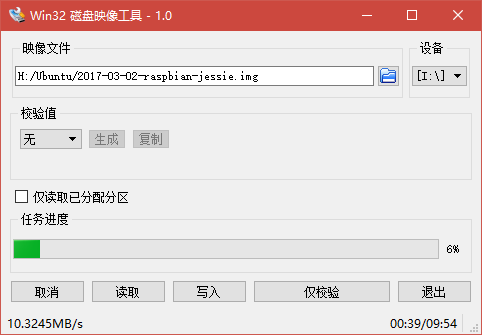
\includegraphics[width=13cm]{figures/win32diskimager.png}
			\caption{Win32DiskImager}
			\label{fig:win32diskimager}
		\end{figure}
		\par $\bullet$ Ubuntu
		\par Ubuntu下使用dd命令进行镜像烧写,首先执行
		\begin{lstlisting}[ language= sh ]
sudo fdisk -l
		\end{lstlisting}
		\par 确认SD卡是否已经挂载,确认已经挂载以后进入镜像文件所在目录执行
		\begin{lstlisting}[ language= sh ]
sudo dd if=2017-03-18-raspbian-jessie-lite.img of=/dev/mmcblk0
		\end{lstlisting}
		\par 其中,\lstinline[language=sh]{of}为SD卡的地址,稍等片刻即可烧写完成。
		\par 2016.11之前的镜像已经默认开启了ssh登陆,插上卡以后插上网线就能够通过ssh登陆(Windows下可以使用putty或者Xshell,Ubuntu下直接在Terminal下执行\lstinline[language=sh]{ssh pi@192.168.199.123}登陆,\lstinline[language=sh]{@}后为树莓派的ip)。
		\par 2016.11之后的镜像默认关闭了ssh登陆,如需使用ssh登陆,则需要在烧写完成以后,SD卡会分为两个分区,于其中\lstinline[language=sh]{boot}目录下新建一个ssh的空白文件(Windows下可以新建文本文件以后删去txt的后缀名,Ubuntu下直接执行\lstinline[language=sh]{touch ssh}即可)。
		\par 树莓派的系统制作完成以后,ssh登陆到树莓派执行
		\begin{lstlisting}[ language= sh ]
sudo raspi-config
		\end{lstlisting}
		\par 会出现如图\ref{fig:raspi_config}所示界面:
		\begin{figure}[htp]
			\centering
			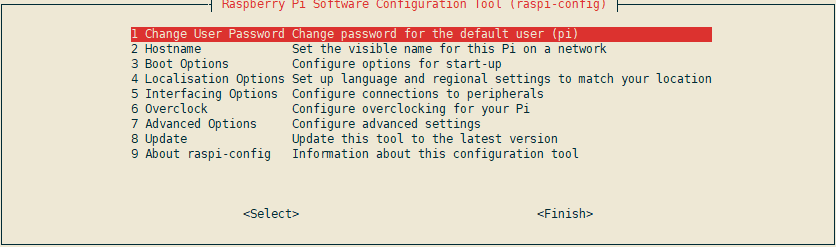
\includegraphics[width=13cm]{figures/raspi-config.png}
			\caption{树莓派配置}
			\label{fig:raspi_config}
		\end{figure}
		\par 其中第一项可以修改用户密码,我们选择\lstinline{Advanced Options}来将系统空间扩展至整个SD卡。
		\begin{figure}[htp]
			\centering
			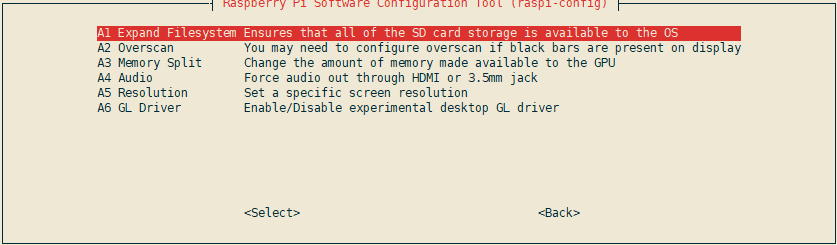
\includegraphics[width=13cm]{figures/raspi-config-expand-filesystem.png}
			\caption{扩展系统空间}
			\label{fig:raspi_config_expand_filesystem}
		\end{figure}
		\par 之后重启系统即可。
		\begin{lstlisting}[ language= sh ]
sudo reboot
		\end{lstlisting}
	\section{软件源}
		\par 树莓派默认使用的官方源服务器国内访问不便,国内使用需要使用镜像站,在此使用的是重庆大学的源,修改\lstinline[language=sh]{/etc/apt/sources.list}为以下内容:
		\begin{lstlisting}[ language= sh ]
deb http://mirrors.ustc.edu.cn/raspbian/raspbian/ jessie main non-free contrib 
deb-src http://mirrors.ustc.edu.cn/raspbian/raspbian/ jessie main non-free contrib
		\end{lstlisting}
		\par 执行
		\begin{lstlisting}[ language= sh ]
sudo apt update
sudo apt upgrade
		\end{lstlisting}
		\par 更新软件,以及各种依赖。
	\section{无线网络配置}
		\par 如果需要将树莓派通过WiFi连接进局域网,则需要配置其无线网络参数,修改\lstinline[language=sh]{/etc/wpa_supplicant/wpa_supplicant.conf}内容为以下内容。
		\begin{lstlisting}
ctrl_interface=DIR=/var/run/wpa_supplicant GROUP=netdev
update_config=1
country=GB

network={
	ssid="your wifi ssid"
	psk="your wifi password"
	priority=5
}
		\end{lstlisting}
		\par 其中:
		\par \lstinline{ssid}为wifi名称。
		\par \lstinline{psk}为wifi密码。
		\par \lstinline{priority}为优先级,数值越大,优先级越高。
		\par 树莓派安装GNU Radio参见\ref{sec:gnuradio}节。
		\par 至此,树莓派的已经基本配置完成。
		% \subsection{镜像备份}
		% TODO:镜像备份

%!TEX root = ../paper.tex
\chapter{环境配置}
	\section{CMake}
		\subsection{简介}
			\par CMake是个开源的跨平台自动化建构系统,它用配置文件控制建构过程(build process)的方式和Unix的Make相似,只是CMake的配置文件取名为CMakeLists.txt。Cmake先产生标准的建构档(如Unix的Makefile或Windows Visual C++的projects/workspaces),然后再依一般的建构方式使用。这使得熟悉某个集成开发环境(IDE)的开发者可以用标准的方式建构他的软件。CMake可以编译源代码、制做程序库、产生适配器(wrapper)、还可以用任意的顺序建构可执行文件,支持二进档和源代码在同一个目录树中建构和二进档在别的目录里建构,因此以很容易从同一个源代码目录树中建构出多个二进档。CMake也支持静态与动态程序库的建构\ucite{ wiki:CMake}。
			\par GNU Radio采用CMake构建,所以简单介绍一下CMake的使用方法,方便后续开发者理解GNU Radio模块的编写以及在此基础上构建自己的应用。
			\par CMake的源码已托管至GitHub(\href{https://github.com/Kitware/CMake.git}{https://github.com/Kitware/CMake.git})。
		\subsection{安装}
			\label{sec:CMake}
			\par 在Ubuntu环境下可以直接执行\lstinline[language=sh]{sudo apt install cmake}来安装。也能使用源码来编译CMake。
			\begin{lstlisting}[ language= sh ]
git clone https://github.com/Kitware/CMake.git
./bootstrap && make && make install
			\end{lstlisting}
			\par 在Windows下可以在CMake官网(\href{https://cmake.org/download/}{https://cmake.org/download/})选择与自己系统版本相对应的版本进行安装。如果使用Visual Studio 2015及以上版本,可以直接用Visual Studio打开项目目录,会自动使用CMake构建相应的解决方案。
		\subsection{构建CMake项目}
			\par CMake要求每个目录下均有一个\lstinline{CMakeLists.txt}文件,一个常见的CMake项目的目录结构如下:
			\dirtree{%
				.1 ..
				.2 app.
				.3 CMakeLists.txt.
				.3 main.cc.
				.3 main.h.
				.2 include.
				.3 CMakeLists.txt.
				.3 test.h.
				.2 lib.
				.3 test\_impl.cc.
				.3 test\_impl.h.
				.2 CMakeLists.txt.
				.2 README.md.
			}
			\par 其中:
			\par \lstinline{app}目录下放置\lstinline{main}函数所在文件,可以同时包含多个将要生成的程序,最终将在\lstinline{./build/app/}目录下生成与该文件同名的可执行文件,在\lstinline{./build/app/}目录下执行\lstinline{./main}即可运行。
			\par \lstinline{include}目录下放置项目所需要的头文件。
			\par \lstinline{lib}目录下为该项目生成的库文件。
			\par \lstinline{README.md}为用Markdown格式书写的说明文档。
			\par 顶层目录下的\lstinline{CMakeLists.txt}内容如下:
			\begin{lstlisting}
project(main)
cmake_minium_required(VERSION 2.6)
aux_source_directories(. DIR_SRC)
include_directories(include)
add_executable(main ${DIR_SRC})
add_subdirectory(lib)
target_link_libraries(main test)
			\end{lstlisting}
			\par \lstinline{/lib/CMakeLists.txt}内容如下:
			\begin{lstlisting}
aux_source_directories(. DIR_TEST_DIR)
add_library(test ${DIR_TEST_DIR})
# add_library(test STATIC ${DIR_TEST_DIR})
			\end{lstlisting}
			\par \lstinline{/include/CMakeLists.txt}文件可以为空,有公共库可以用\lstinline[language=sh]{install(file name)}来安装进系统环境。
			\par 编译运行
			\begin{lstlisting}[ language = sh ]
mkdir build
cd build
cmake ..
make
			\end{lstlisting}
			\par 便会在\lstinline{/build/build/app}目录下生成相应的可执行文件。在使用git时进行版本控制注意在gitignore中添加build目录,以免git对编译后产生的文件进行跟踪,以免编译一次产生一次更改,造成版本库的混乱。有众多的开源项目基于CMake构建,使用这些程序时编译完成以后还需要使用以下命令来将其置入系统路径,使其能够在命令行下直接执行。
			\begin{lstlisting}
sudo make install
			\end{lstlisting}
			\par 如果编译的动态库还需要将其链接:
			\begin{lstlisting}[ language= sh ]
sudo ldconfig
			\end{lstlisting}
	\section{Boost C++ Libraries}
		\subsection{简介}
			\par Boost C++ 库(Libraries)是一组扩充C++功能的经过同行评审(Peer-reviewed)且开放源代码程序库。大多数的函数为了能够以开放源代码、封闭项目的方式运作,而授权于Boost软件许可协议(Boost Software License)之下。许多Boost的开发人员是来自C++标准委员会,而部分的Boost库成为C++的TR1标准之一\ucite{ wiki:Boost}。
			\par GNU Radio与gr-dvbt中调用了Boost库中的众多函数,需要安装该库才能够进行编译,执行以下命令进行安装。
			\begin{lstlisting}[ language= sh ]
sudo apt install libboost-all-dev
			\end{lstlisting}
			\par Boost的源码已托管于GitHub(\href{https://github.com/boostorg}{https://github.com/boostorg})。
	\section{Doxygen}
		\subsection{简介}
			\par Doxygen是一个C++、C、Java、Objective-C、Python、IDL(CORBA和Microsoft flavors)、Fortran、VHDL、PHP、C\#和D语言的文档生成器。可以在大多数类Unix以及Mac OS X和Microsoft Windows上运行。Doxygen文档是直接写在源代码中,因此比较容易保持更新。Doxygen支持交叉引用文档和源代码,使文件的读者可以很容易地引用实际的源代码\ucite{ wiki:Doxygen}。
			\par GNU Radio的API文档(\href{https://gnuradio.org/doc/doxygen/index.html}{https://gnuradio.org/doc/doxygen/index.html})由Doxygen生成。
			\par 在编写程序的过程中使用符合Doxygen规范的注释块,如有需要,构建时可以使用Doxygen生成如图\ref{fig:doxygen_gnuradio}的说明文档以及如图\ref{fig:doxygen_dvbt_map}调用关系图。
			\begin{figure}[htbp]
				\centering
				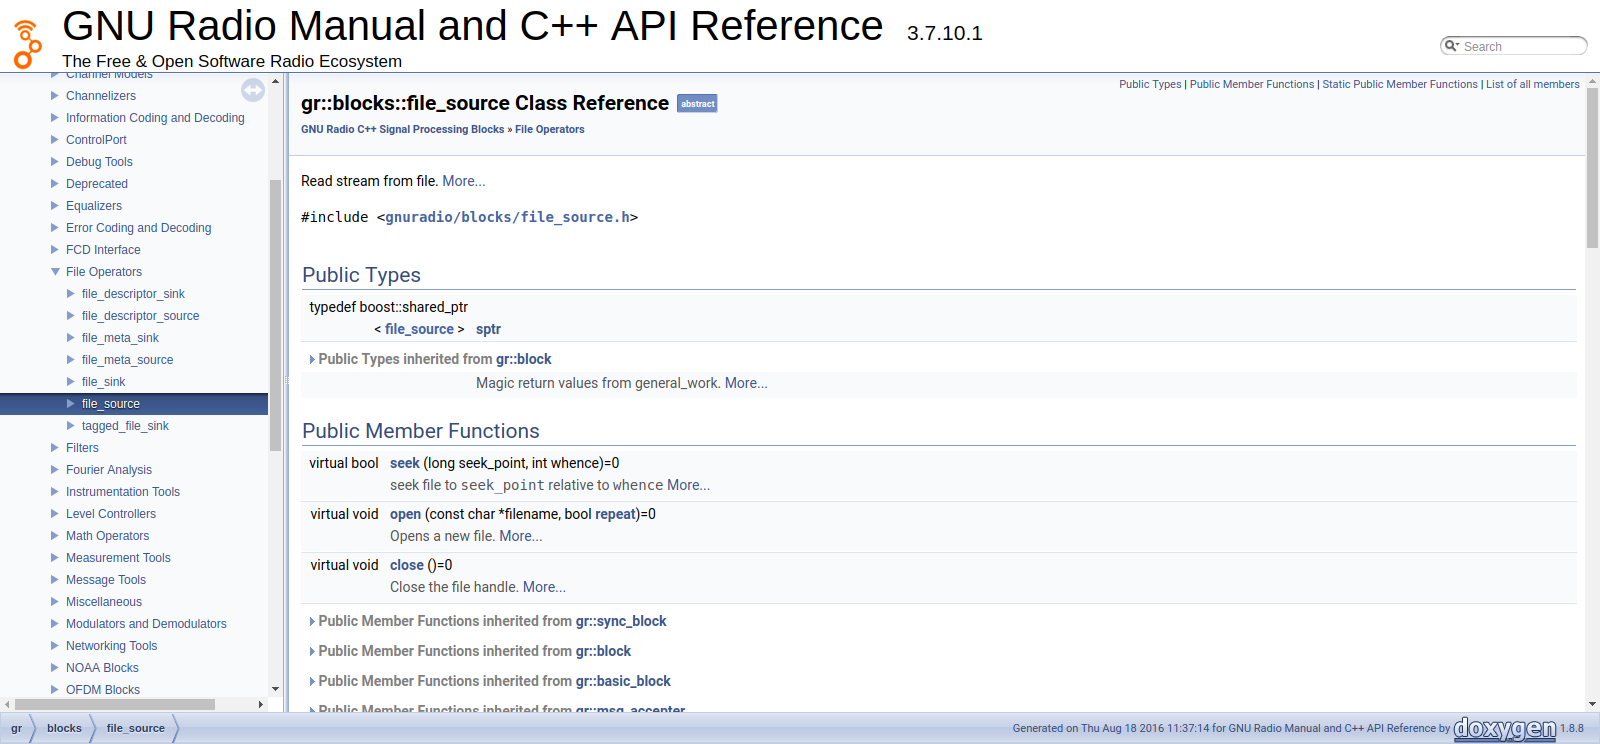
\includegraphics[width=13cm]{figures/doxygen_gnuradio.png}
				\caption{Doxygen生成的GNU Radio说明文档}
				\label{fig:doxygen_gnuradio}
			\end{figure}
			\begin{figure}[htbp]
				\centering
				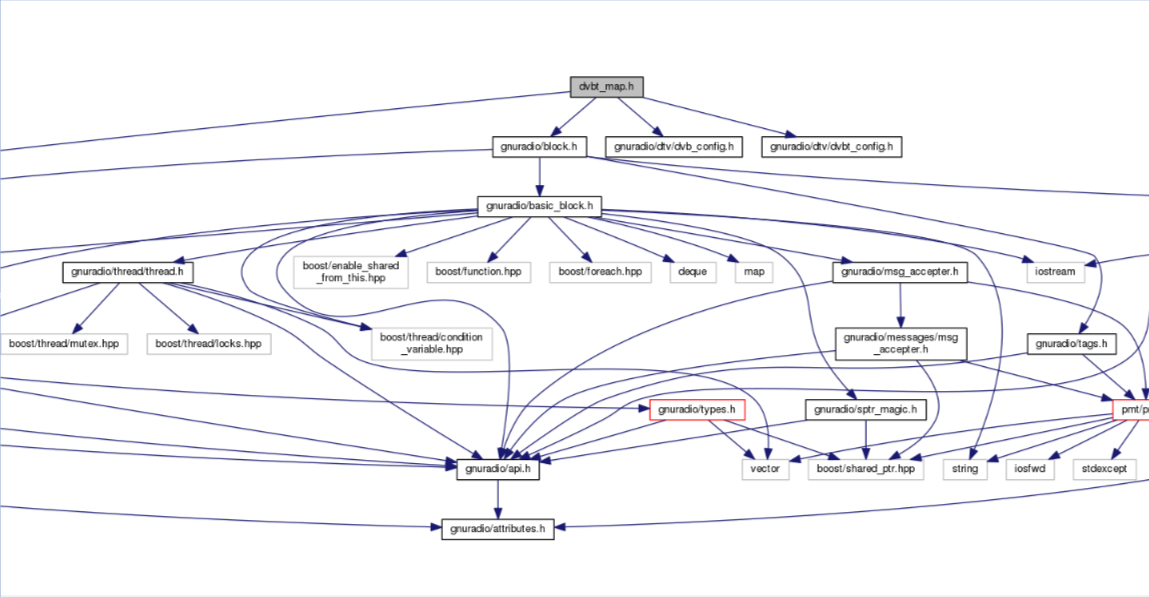
\includegraphics[width=13cm]{figures/doxygen_dvbt_map.png}
				\caption{Doxygen生成的调用关系图}
				\label{fig:doxygen_dvbt_map}
			\end{figure}
			\par Doxygen的源码已托管于GitHub(\href{https://github.com/doxygen/doxygen}{https://github.com/doxygen/doxygen})。
		\subsection{使用方法}
			\par 在文件中使用Doxygen规范的注释\ucite{ wiki:Doxygen}。
			\par 一般文件:
			\begin{lstlisting}
/**
* <A short one line description>
*
* <Longer description>
* <May span multiple lines or paragraphs as needed>
*
* @param  Description of method's or function's input parameter
* @param  ...
* @return Description of the return value
*/
			\end{lstlisting}
			\par 头文件:
			\begin{lstlisting}
/*!
* <A short one line description>
*
* <Longer description>
* <May span multiple lines or paragraphs as needed>
*
* @param  Description of method's or function's input parameter
* @param  ...
* @return Description of the return value
*/
			\end{lstlisting}
			\par 在工程目录下执行\lstinline[language=sh]{doxygen -g}生成Doxyfile,修改\lstinline{OUTPUT_DIRECTORY}为自己想要的生成目录与其他参数,最后执行\lstinline{doxygen Doxyfile}即可生成\lstinline{latex}和\lstinline{html}目录,打开\lstinline{html}目录下的\lstinline{index.html}即可看到生成的网页格式的说明文档以及文件间的调用关系图,在\lstinline{latex}目录下运行\lstinline{./make}还可以生成pdf文件。
			\par Doxygen还能嵌入到CMake中,在\lstinline{CMakeLists.txt}中添加以下命令
			\begin{lstlisting}
# add a target to generate API documentation with Doxygen

FIND_PACKAGE(Doxygen)
OPTION(BUILD_DOCUMENTATION "Create and install the HTML based API documentation (requires Doxygen)" ${DOXYGEN_FOUND})

IF(BUILD_DOCUMENTATION)
	IF(NOT DOXYGEN_FOUND)
		MESSAGE(FATAL_ERROR "Doxygen is needed to build the documentation.")
	ENDIF()

	SET(doxyfile_in ${CMAKE_CURRENT_SOURCE_DIR}/Doxyfile.in)
	SET(doxyfile ${CMAKE_CURRENT_BINARY_DIR}/Doxyfile)

	CONFIGURE_FILE(${doxyfile_in} ${doxyfile} @ONLY)

	ADD_CUSTOM_TARGET(doc
		COMMAND ${DOXYGEN_EXECUTABLE} ${doxyfile}
		WORKING_DIRECTORY ${CMAKE_CURRENT_BINARY_DIR}
		COMMENT "Generating API documentation with Doxygen"
		VERBATIM)

	INSTALL(DIRECTORY ${CMAKE_CURRENT_BINARY_DIR}/html DESTINATION share/doc)
ENDIF()
			\end{lstlisting}
			\par 使用CMake生成\lstinline{makefile}以后,可以使用\lstinline{make doc}来生成API文档。
	\section{Python}
		\subsection{简介}
			\par Python,是一种面向对象、解释型的计算机程序语言。它包含了一组功能完备的标准库,能够轻松完成很多常见的任务。它的语法简单,与其它大多数程序设计语言使用大括号不一样,它使用缩进来定义语句块,经常被当作脚本语言用于处理系统管理任务和网络程序编写,然而它也非常适合完成各种高级任务。Python支持命令式程序设计、面向对象程序设计、函数式编程、面向侧面的程序设计、泛型编程多种编程范式\ucite{ wiki:Python}。
			\par Python简单的语法能够让开发者专注于算法,而不用去纠结语法上的问题,其众多的第三方库也给开发者带来了极大的便利,诸如用于科学计算的NumPy库已经能够替代Matlab的一些功能,所以Python语言具有很高的开发效率,已经被广泛地应用于机器学习、科学计算、Web后端、数字图像处理等众多领域。可以预见,在不久的将来也会在数字信号处理与通信工程领域大放异彩。
			\par GNU Radio采用Python来连接各个模块,在模块间传递参数,支持直接Python编程,但是由于Python执行效率较低,所以底层采用C++来提高性能,通过SWIG将C++类跟函数封装为Python中的模块,实现了性能与效率的综合。
			\par 一个不错的Python学习网站是廖雪峰的官方网站(\href{http://www.liaoxuefeng.com/}{http://www.liaoxuefeng.com/}),此处不再赘述。
			\par Python源码可以从\href{https://www.python.org/downloads/source/}{https://www.python.org/downloads/source/}下载。
	% \section{SWIG}
	% 	\subsection{简介}
	% 		\par SWIG是个帮助使用C或者C++编写的软件能与其它各种高级编程语言进行嵌入联接的开发工具。SWIG能应用于各种不同类型的语言包括常用脚本编译语言例如Perl, PHP, Python, Tcl, Ruby and PHP。SWIG普遍应用于创建高级语言解析或汇编程序环境,用户接口,作为一种用来测试C/C++或进行原型设计的工具\ucite{ wiki:SWIG}。
	% 		\par GNU Radio使用C++编写底层函数以实现性能最大化,使用SWIG将其中公有函数封装为Python的模块,极大的方便了开发者直接使用Python作为开发语言。GNU Radio的SWIG文件为\lstinline[language=sh]{swig}目录下的\lstinline[language=sh]{*.i}文件。
	% 		\par SWIG的源码已托管于GitHub(\href{https://github.com/swig/swig}{https://github.com/swig/swig})。
	% 		% TODO:用法
	\section{USRP}
		\subsection{简介}
			\par 通用软件无线电外设(USRP)是由Ettus Research及其母公司National Instruments设计和销售的一系列软件定义无线电设备。由Matt Ettus领导的团队开发,USRP产品系列旨在成为软件无线电相对便宜的硬件平台,已经被研究实验室,大学和业余爱好者广泛使用。大多数USRP通过高速链路连接到主机,主机软件用于控制USRP硬件和发送/接收数据,一些USRP模型还将主机的一般功能与嵌入式处理器集成,从而允许USRP设备以独立的方式运行。USRP系列设计之初便有很高的可修改性,许多产品是开源硬件,所有USRP型号的电路板原理图均可免费下载,所有USRP产品均采用开源的UHD驱动程序进行控制。USRP通常与GNU Radio软件套件一起使用,以创建复杂的软件定义无线电系统\ucite{ wiki:USRP}。
			\begin{figure}[htbp]
				\centering
				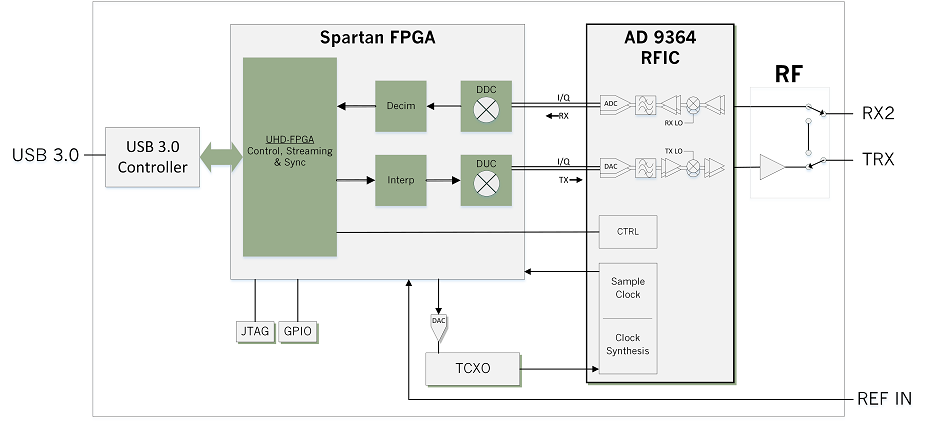
\includegraphics[width=13cm]{figures/USRP_B200mini_BD.png}
				\caption{USRP\_B200mini\_原理图}
				\label{fig:USRP_B200mini_原理图}
			\end{figure}
			\par UHD的源码已托管于GitHub(\href{https://github.com/EttusResearch/uhd}{https://github.com/EttusResearch/uhd})。
		\subsection{UHD}
			\par UHD是适用于USRP相关设备的开源的驱动程序,安装完成GNU Radio以后会自动安装UHD相关软件,USRP B200 mini需要UHD3.9.0及以上版本,使用版本过低会导致USRP无法识别。UHD提供了一些简单信号发生函数,能够用来实现一些简单的测试。
			\par 首次使用需要执行
			\begin{lstlisting}[ language = sh ]
uhd_images_downloader
			\end{lstlisting}
			\par 来下载USRP需要的镜像,以便之后的使用。
			\par 执行
			\begin{lstlisting}[ language = sh ]
uhd_siggen -f 900000000
			\end{lstlisting}
			\par 来产生一个如图\ref{fig:uhd_siggen}的正弦波。
			\begin{figure}[htp]
				\centering
				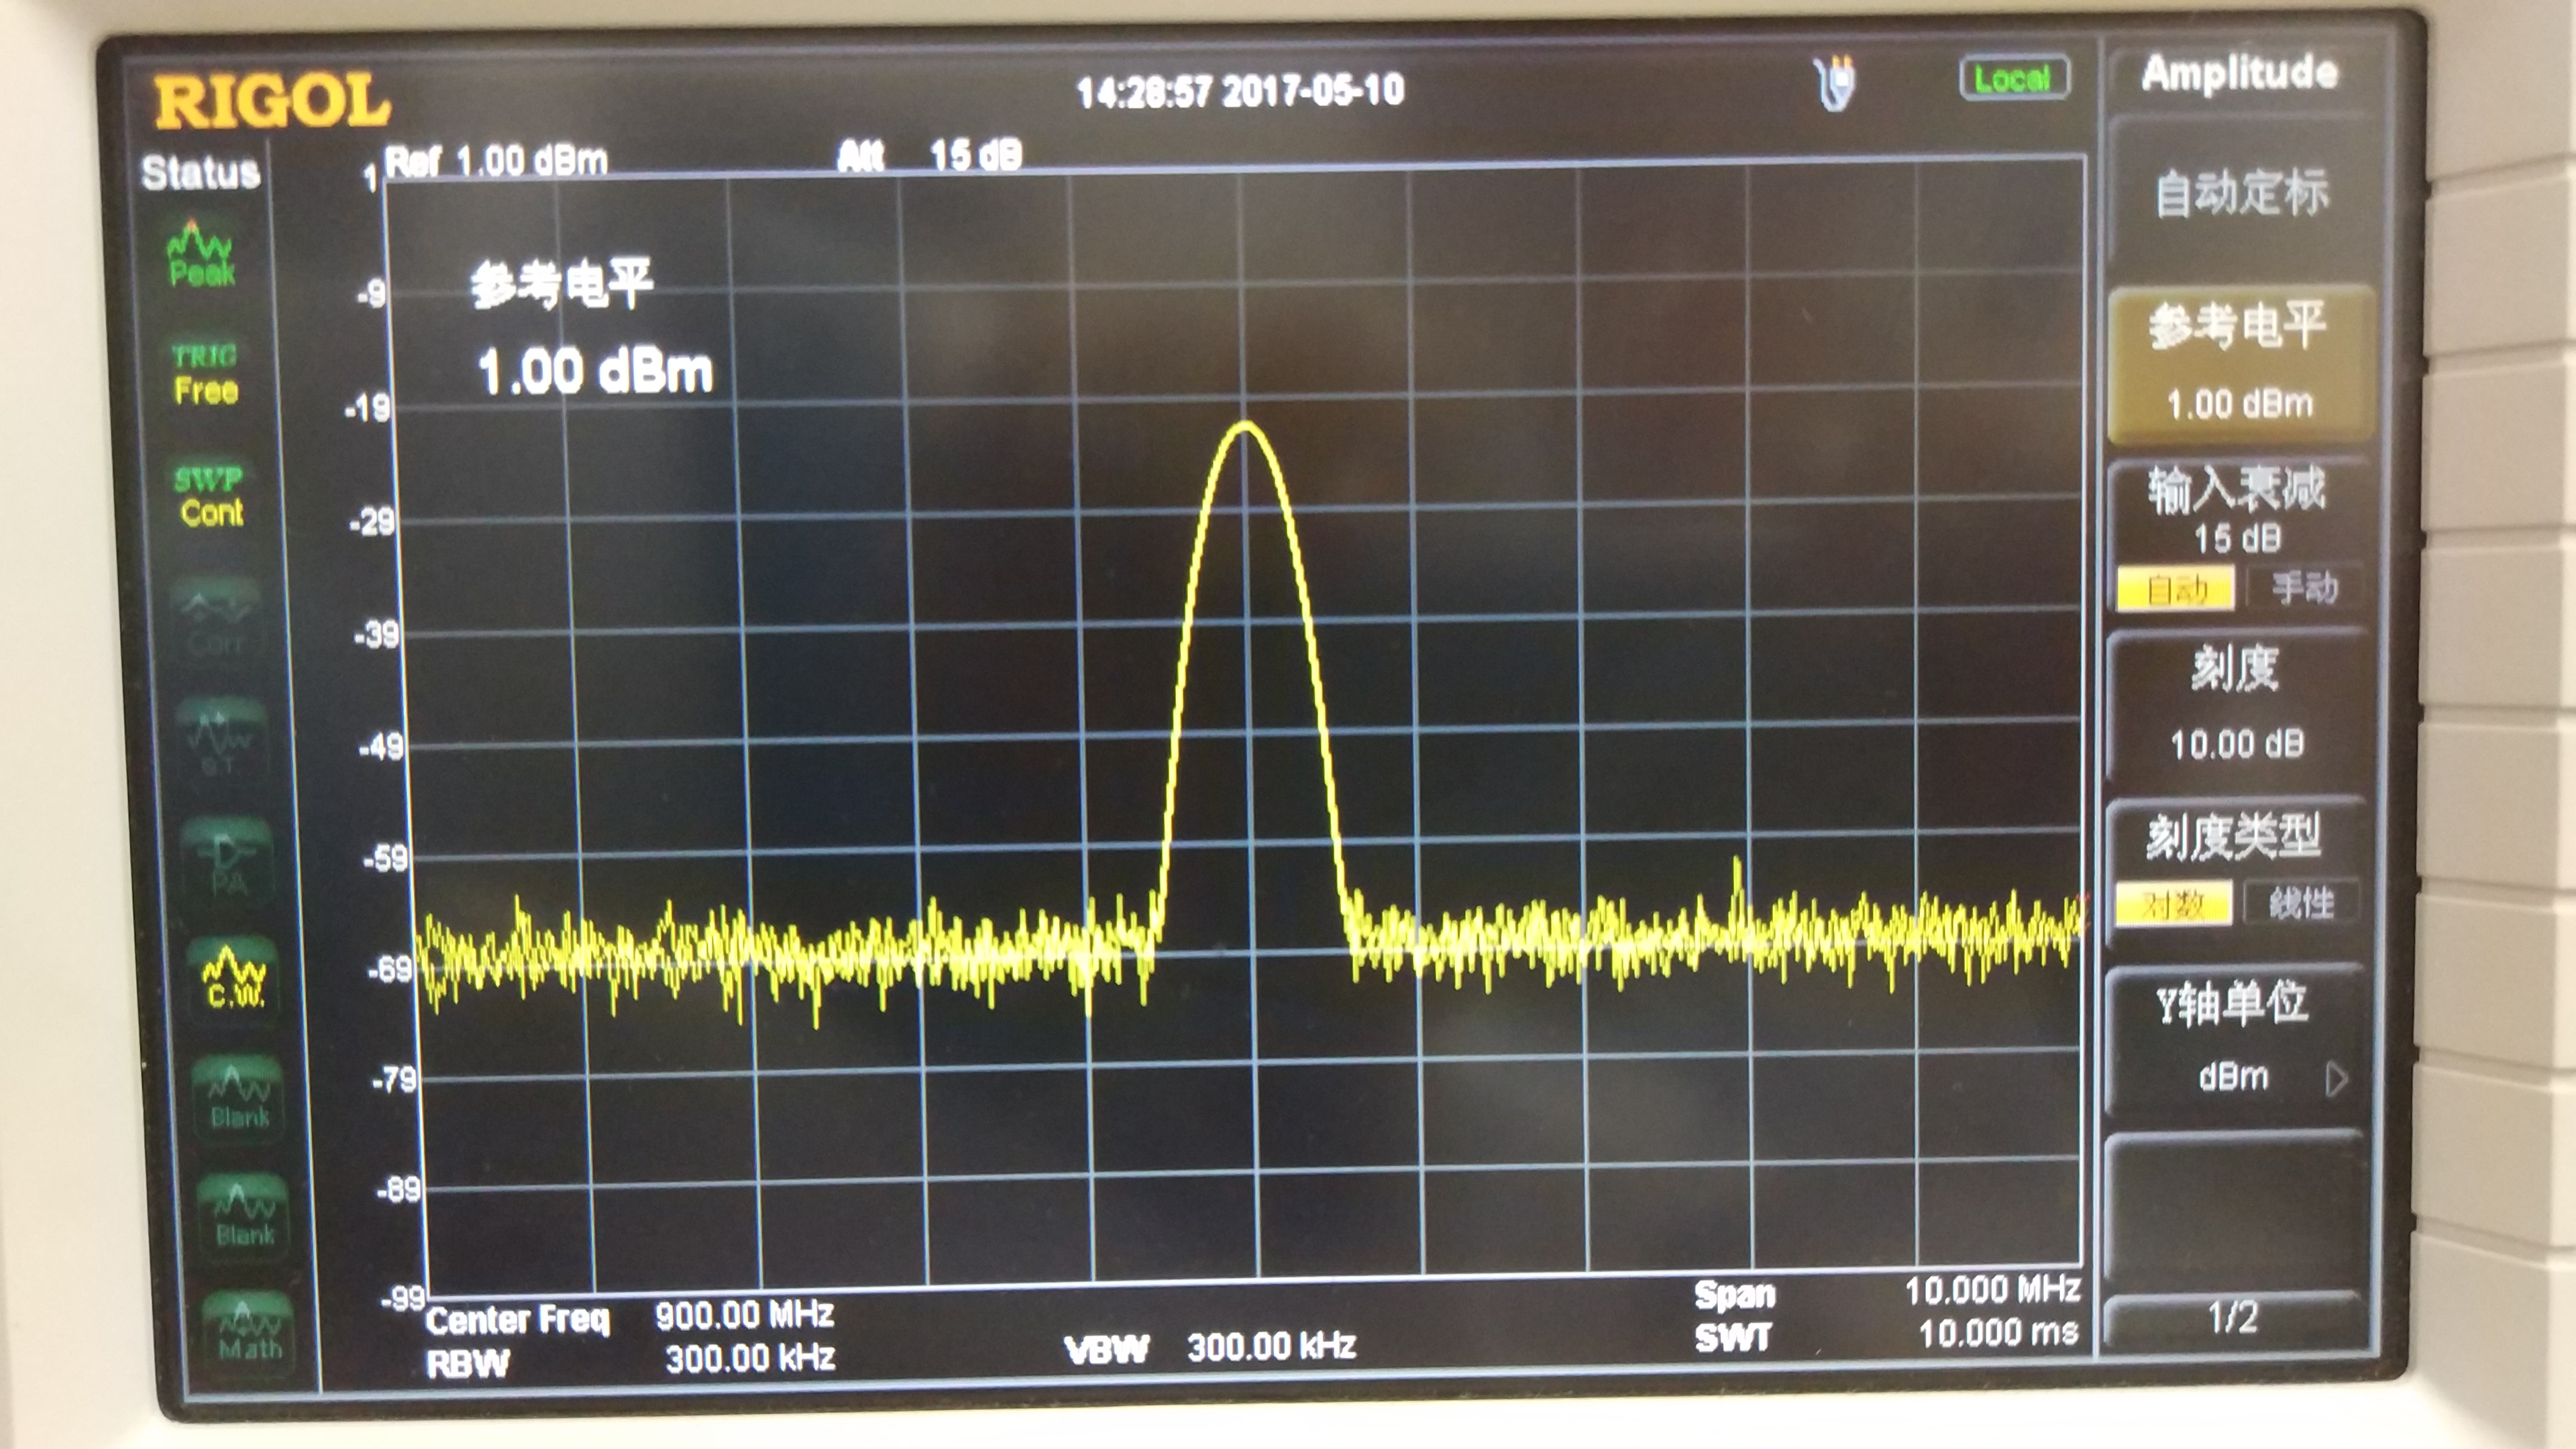
\includegraphics[width=13cm]{figures/uhd_siggen.jpg}
				\caption{uhd\_siggen}
				\label{fig:uhd_siggen}
			\end{figure}
			\par 或者执行
			\begin{lstlisting}[ language = sh ]
uhd_siggen_gui -f 900000000
			\end{lstlisting}
			\par 来运行一个如图\ref{fig:uhd_siggen_gui}的基于GNU Radio的GUI界面。
			\begin{figure}[htp]
				\centering
				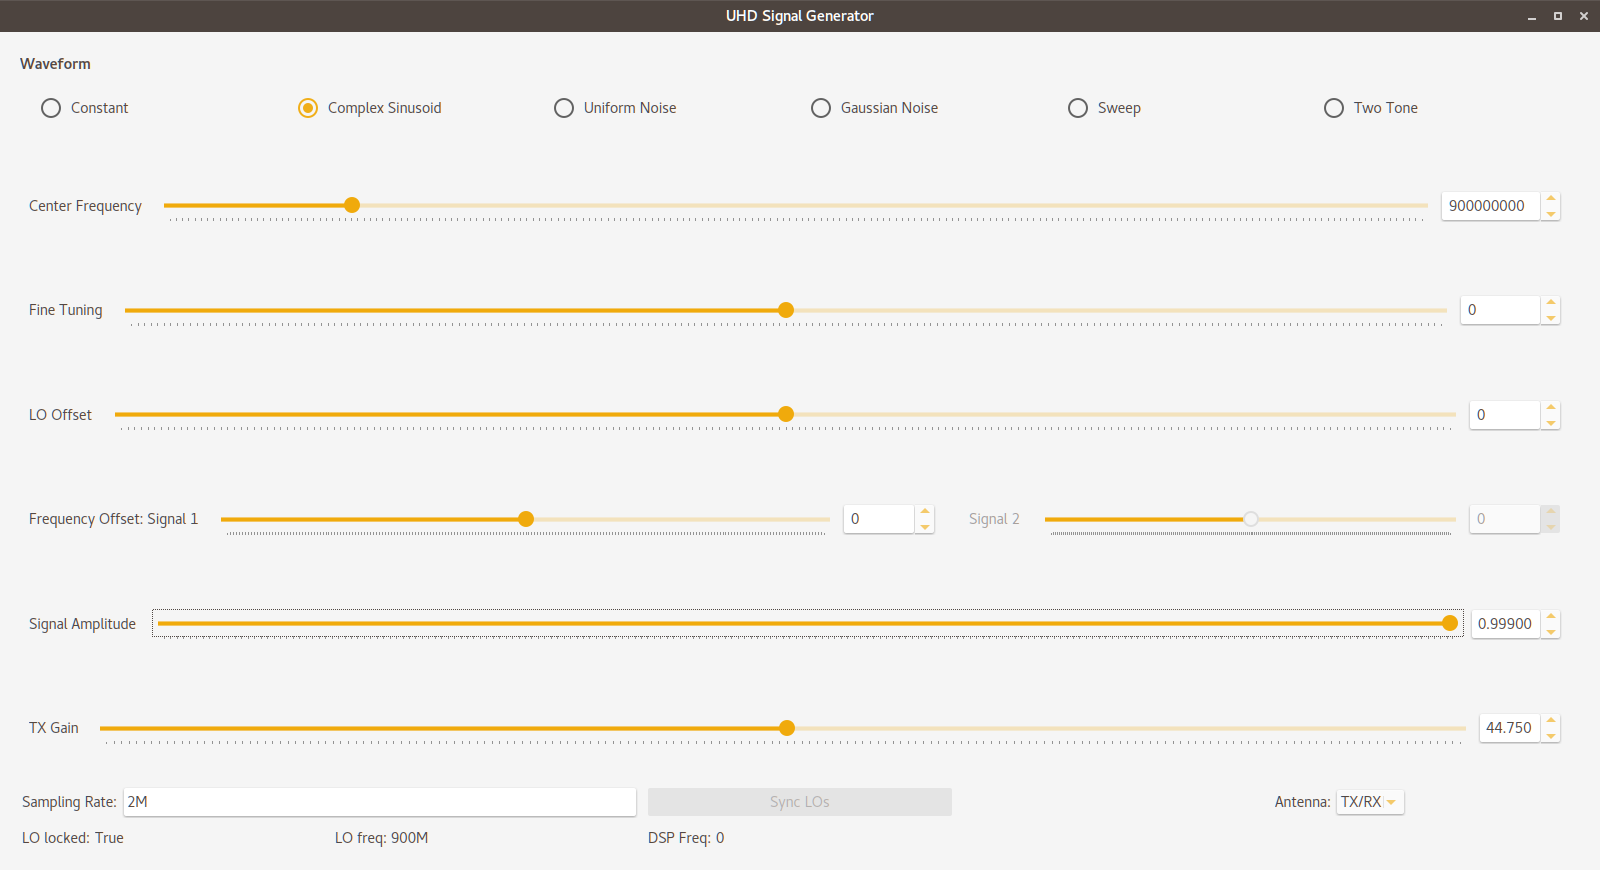
\includegraphics[width=13cm]{figures/uhd_siggen_gui.png}
				\caption{uhd\_siggen\_gui}
				\label{fig:uhd_siggen_gui}
			\end{figure}
	% \section{gqrx}
	% 	\subsection{简介}
	% 		\par gqrx是由GNU Radio和Qt图形工具包提供支持的开源软件定义无线电接收器(SDR),用来通过USRP接收无线电信号,可以直接接收FM广播,并提供直观的瀑布图,可以作为没有频谱仪情况下的替代品。
	% 		\par gqrx支持许多SDR硬件,包括Airspy,Funcube Dongles,rtl-sdr,HackRF和USRP设备,gqrx是免费软件,根据GNU通用公共许可证许可,允许任何人修复和修改它以供使用。
	% 		\begin{figure}[htbp]
	% 			\centering
	% 			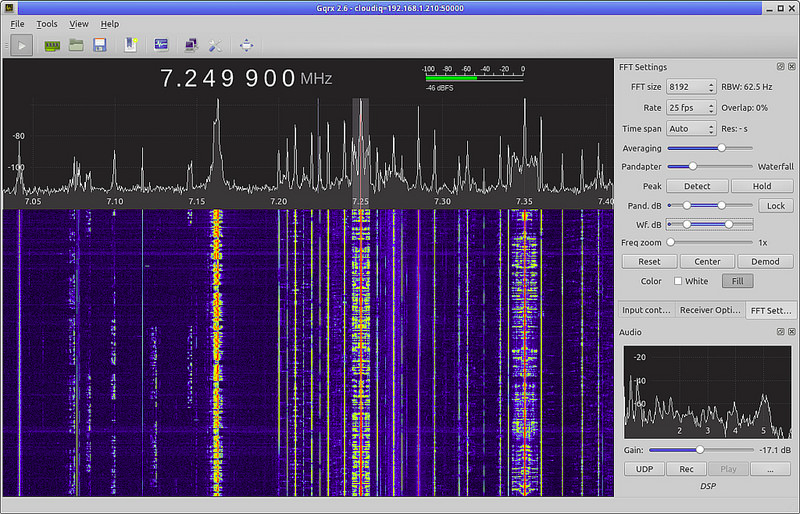
\includegraphics[width=13cm]{figures/gqrx.png}
	% 			\caption{gqrx运行截图}
	% 			\label{fig:gqrx运行截图}
	% 		\end{figure}
	% 		\par gqrx的源码已托管于GitHub(\href{https://github.com/csete/gqrx}{https://github.com/csete/gqrx})。
	\section{git}
		\subsection{简介}
			\par git是用于Linux内核开发的版本控制工具。与CVS、Subversion一类的集中式版本控制工具不同,它采用了分布式版本库的作法,不需要服务器端软件,就可以运作版本控制,使得源代码的发布和交流极其方便。git的速度很快,这对于诸如Linux内核这样的大项目来说自然很重要。git最为出色的是它的合并追踪(merge tracing)能力\ucite{ wiki:Git}。
			\par GNU Radio使用git进行版本控制,在进行源码查看编辑的时候使用git能大大提高开发效率,在此简要介绍其使用方法。
			\par git的一个仓库由三个区组成:工作区,暂存区,版本库。我们平常编写程序的叫做工作区,在工作区中编写程序,修复bug,然后将修改后的文件通过\lstinline[language=sh]{git add -p <file>}	命令添加到暂存区,检查暂存区没有错误以后通过\lstinline[language=sh]{git commit -m "some comments"}命令将修改提交至版本库,如果存在远程仓库还需要执行\lstinline[language=sh]{git push}命令来将修改提交至远程仓库。
			\par 以上是一个正常的提交流程,我们可以通过\lstinline[language=sh]{git log}来查看所有的\lstinline[language=sh]{commit},并通过\lstinline[language=sh]{git reset --hard <your commit flag>}来回退至相应的版本。
			\par 一个好的习惯是在添加新功能或者修复某一个bug时执行\lstinline[language=sh]{git checkout -b fix}创建一个名为\lstinline[language=sh]{fix}的分支,在该分支中修改bug,修改完成并测试通过以后\lstinline[language=sh]{git commit -m "some comments"}将修改提交至本地仓库,再执行\lstinline[language=sh]{git checkout master}并执行\lstinline[language=sh]{git merge fix}来将修改合并至主分支,这样可以在不影响主分支的情况进行bug的修复和新功能的添加。在GitHub上可能还需要执行pull request来将修改提交至源仓库。
			\par git的源码已托管于GitHub(\href{https://github.com/git/git}{https://github.com/git/git})。
		\subsection{常用命令}
			\par $\bullet$ \lstinline[language=sh]{git config --global user.name "Your name"}
			\par 使用仓库之前得先告诉git你是谁,谁提交了接下来的修改。
			\par $\bullet$ \lstinline[language=sh]{git config --global user.email "email@example.com"}
			\par git是外国人开发的,较为正式的联系方式是电子邮件。
			\par $\bullet$ \lstinline[language=sh]{git add -p <file>}
			\par 将文件和修改提交至暂存区,可以使用\lstinline[language=sh]{git add .}命令将所有文件提交至暂存区。
			\par $\bullet$ \lstinline[language=sh]{git commit -m "some comments"}
			\par 将文件和修改提交至本地仓库,并添加一些批注。
			\par $\bullet$ \lstinline[language=sh]{git status}
			\par 显示仓库当前状态。
			\par $\bullet$ \lstinline[language=sh]{}git log
			\par 显示提交日志,可以通过添加\lstinline[language=sh]{--pretty=oneline}参数来格式化输出信息。
			\par $\bullet$ \lstinline[language=sh]{git reset --hard 130f101}
			\par 版本回退,最后的为\lstinline[language=sh]{git log}中的唯一标识,也可以使用\lstinline[language=sh]{HEAD}来撤销更改,回退到当前版本。
			\par $\bullet$ \lstinline[language=sh]{git checkout -- <file>}
			\par 丢弃工作区的修改,回到最近一次的\lstinline[language=sh]{commit}或者\lstinline[language=sh]{add}的状态,该命令可以在\lstinline[language=sh]{git status}中提示。
			\par $\bullet$ \lstinline[language=sh]{git push origin master}
			\par 将修改提交至远程仓库,可以添加多个远程仓库,可以指定分支。
			\par $\bullet$ \lstinline[language=sh]{git diff}
			\par 显示文件于版本库的差异。
			\par $\bullet$ \lstinline[language=sh]{git fetch}
			\par 获取远程仓库的最新版本。
			\par $\bullet$ \lstinline[language=sh]{git pull}
			\par 获取远程仓库的最新版本,并与本地仓库合并。
			\par $\bullet$ \lstinline[language=sh]{git branch dev}
			\par 创建分支。
			\par $\bullet$ \lstinline[language=sh]{git checkout dev}
			\par 切换至dev分支,可以使用\lstinline[language=sh]{git checkout -b dev}来创建并切换至dev分支。
			\par $\bullet$ \lstinline[language=sh]{git merge dev}
			\par 合并指定分支至当前分支。
			\par 在众多教程中,廖雪峰的官方网站(\href{http://www.liaoxuefeng.com/}{http://www.liaoxuefeng.com/})很适合初学者,深入浅出的讲解了使用git过程中常用的许多命令。
			% \subsection{版本控制}
		% \subsection{GitHub}
		% 	\par GitHub是一个通过Git进行版本控制的软件源代码托管服务,由GitHub公司(曾称Logical Awesome)的开发者Chris Wanstrath、PJ Hyett和Tom Preston-Werner使用Ruby on Rails编写而成。GitHub同时提供付费账户和免费账户,这两种账户都可以创建公开的代码仓库,但是付费账户还可以创建私有的代码仓库。根据在2009年的Git用户调查,GitHub是最流行的Git访问站点。除了允许个人和组织创建和访问保管中的代码以外,它也提供了一些方便社会化共同软件开发的功能,即一般人口中的社区功能,包括允许用户追踪其他用户、组织、软件库的动态,对软件代码的改动和bug提出评论等\ucite{ wiki:GitHub}。
		% 	\par GitHub的使用与git并无太多区别。
		% 	\par 本设计使用的众多开源库、软件均已托管于GitHub。
	% \section{Docker}
	% 	\subsection{简介}
	% 		\par Docker是一个开放源代码软件项目,让应用程序布署在软件容器下的工作可以自动化进行,借此在Linux操作系统上,提供一个额外的软件抽象层,以及操作系统层虚拟化的自动管理机制。Docker利用Linux核心中的资源分脱机制,例如cgroups,以及Linux核心名字空间(name space),来创建独立的软件容器(containers)。这可以在单一Linux实体下运作,避免引导一个虚拟机造成的额外负担。Linux核心对名字空间的支持完全隔离了工作环境中应用程序的视野,包括进程树、网络、用户ID与挂载文件系统,而核心的cgroup提供资源隔离,包括CPU、存储器、block I/O与网络。从0.9版本起,Dockers在使用抽象虚拟是经由libvirt的 LXC与systemd - nspawn提供界面的基础上,开始包括libcontainer库做为以自己的方式开始直接使用由Linux核心提供的虚拟化的设施\ucite{ wiki:Docker}。
	% 		\par 在构建应用时,如果在实机上进行运行测试,很容易因为依赖的问题导致应用无法正常运行,严重时会造成系统的崩溃。Docker提供了一个虚拟的环境来构建自己的应用,同时也能够与git进行版本控制与回滚,在Docker中构建应用也能更快的部署应用。需要大规模部署应用时只需要从仓库中拉取自己需要的环境以及版本,进行少量的配置即可运行。
	% 		\par 本设计由于时间问题并未采用Docker来管理系统镜像版本,在修改系统环境的过程中走了不少弯路,后续开发者可以一开始就在Docker的环境下开发软件,或者在安装Ubuntu时使用LVM,创建快照省去因为系统环境配置出错而频繁的重装系统,保证一个相对纯净的开发环境,同时其他开发者可以直接拉取该镜像以进行二次开发。
	% 		% \subsection{构建容器}
	% 		% TODO: 构建容器
	\section{GNU Radio}
		\label{sec:gnuradio}
		\subsection{简介}
			\par GNU Radio 是免费开源的软件开发工具套件。它提供构建软件无线电所需的信号运行和处理的模块,用它可以在唾手可得的低成本的外部射频(RF)硬件和通用微处理器上、或无硬件的模拟环境中实现软件定义无线电。这套套件广泛用于业余爱好者,学术机构和商业机构用来研究和构建无线通信系统。
			\par GNU Radio 可以进行各类信号处理。可以使用它编写应用程序从数据流中获取数据或将数据传输到数据流中,然后使用硬件将其发射出去。GNU Radio 具有滤波器、通道编码、同步单元、均衡单元(equalizer)、解调器、声音合成机(vocoder)、解码器(decoder)等很多单元(使用 GNU Radio 术语,这些被称作功能块 - blocks),这些单元也都是无线电系统中的常见部件单元。更重要的是,它还具有连接这些功能模块的方法及管理在这些功能块间传输数据的策略。GNU Radio 的应用主要是用 Python 编程语言来编写的。但是其核心信号处理模块是 C++ 在带浮点运算的微处理器上构建的。因此,开发者能够简单快速的构建一个实时、高容量的无线通信系统\ucite{what_is_gnuradio}。
			\par GNU Radio的使用方法类似于Matlab中的SimuLink,通过拖动框图来构建通信系统,并能够生成一个Python文件,如果使用No Gui就能够生成命令行下可以直接运行的程序。因为其有友好的GUI界面,此处不再赘述使用方法。
		\subsection{安装}
			\par GNU Radio安裝有两种方式:源码编译和通过包管理程序安装,包管理程序安装方式包括两种:apt-get和PyBOMBS。
			\par\noindent $\bullet$ 源码编译
			\par GNU Radio需要的依赖参看\href{https://gnuradio.org/doc/doxygen/build\_guide.html}{https://gnuradio.org/doc/doxygen/build\_guide.html},所有依赖均可以通过apt-get的方式进行安装,这种方式可以保证软件版本较新,但是安装时间较长,编译时间可能长达数小时,所以大多数情况下采用包管理程序安装。
			\par\noindent $\bullet$ 包管理安装
			\par\noindent \qquad$\circ$ apt-get
			\par Ubuntu:
			\par Ubuntu 16.04的源中提供的版本为3.7.9,需要手动编译gr-dvbt(参见\ref{sec:gr-dvbt_compile}节),Ubuntu 17.04中的源已经更新至3.7.10,已经内置了gr-dvbt,不需要再手动编译了,安装GNU Radio时推荐使用新立得包管理软件(Synaptic)。
			\par 树莓派:
			\par 树莓派默认的软件源为jessie,提供的最新版本为3.7.5,需要手动编译gr-dvbt(参见\ref{sec:gr-dvbt_compile}节)。如果需要安装3.7.10版本,需要切换软件源为stretch源(stretch为testing源),修改\lstinline[language=sh]{/etc/apt/source.list}文件,将其中的jessie修改为stretch。
			\begin{lstlisting}
deb http://mirrors.ustc.edu.cn/raspbian/raspbian/ stretch main non-free contrib 
deb-src http://mirrors.ustc.edu.cn/raspbian/raspbian/ stretch main non-free contrib
			\end{lstlisting}
			\par 修改完成后执行
			\begin{lstlisting}
sudo apt update
sudo apt install gnuradio-dev
			\end{lstlisting}
			\par 安装完成之后使用python测试,gnuradio需要Python 2环境,在Python 3环境下无法运行。
			\begin{lstlisting}[ language= sh ]
Python 2.7.13 (default, Jan 19 2017, 14:48:08)
[GCC 6.3.0 20170118] on linux2
Type "help", "copyright", "credits" or "license" for more information.
>>> import gnuradio
>>>
			\end{lstlisting}
			\par 如果没有出现\lstinline[language=sh]{no module named gnuradio}则表示安装成功。
			\par\noindent \qquad$\circ$ PyBOMBS
			\par 安装PyBOMBS
			\begin{lstlisting}[ language= sh ]
sudo pip install PyBOMBS
			\end{lstlisting}
			\par 或者
			\begin{lstlisting}[ language= sh ]
git clone https://github.com/gnuradio/pybombs.git
cd pybombs
sudo python setup.py install
			\end{lstlisting}
			\par 添加PyBOMBS源
			\begin{lstlisting}[ language= sh ]
pybombs recipes add gr-recipes git+https://github.com/gnuradio/gr-recipes.git  
pybombs recipes add gr-etcetera git+https://github.com/gnuradio/gr-etcetera.git
			\end{lstlisting}
			\par 配置安装参数
			\begin{lstlisting}[ language= sh ]
pybombs prefix init ~/prefix/default/
			\end{lstlisting}
			\par 安装GNU Radio
			\begin{lstlisting}[ language= sh ]
pybombs install gnuradio
			\end{lstlisting}
			\par 运行GNU Radio Companion
			\begin{lstlisting}[ language= sh ]
pybombs run gnuradio-companion
			\end{lstlisting}
		\subsection{gr-dvbt编译}
			\label{sec:gr-dvbt_compile}
			\par gr-dvbt源码已托管于GitHub(\href{https://github.com/BogdanDIA/gr-dvbt}{https://github.com/BogdanDIA/gr-dvbt})。
			\par 3.7.9及以下版本的GNU Radio需要从源码编译,首先安装相关依赖,一般情况下需要以下依赖:
			\begin{lstlisting}[ language= sh ]
sudo apt install log4cpp libboost-all-dev swig git cmake
			\end{lstlisting}
			\par 编译并运行
			\begin{lstlisting}[ language= sh ]
git clone https://github.com/BogdanDIA/gr-dvbt.git
cd gr-dvbt
mkdir build
cd build
cmake ../
make && sudo make install
			\end{lstlisting}
			\par 如果是第一次安装还需要链接动态库
			\begin{lstlisting}[ language= sh ]
sudo ldconfig
			\end{lstlisting}
			\par\noindent $\bullet$ 树莓派
			\par 由于gr-dvbt使用了维特比解码,并且在其中调用了\lstinline{xmmintrin.h},使用x86平台下的汇编来进行计算加速,导致无法在树莓派平台上成功编译。但是,维特比解码仅在接收端使用,所以可以注释其中与维特比有关的代码段来成功编译,并运行发射端程序。
			\par \lstinline{/lib/CMakeLists.txt}中注释以下行
			\begin{lstlisting}
......
# viterbi_decoder_impl.cc
# d_viterbi.c
......
# ${CMAKE_CURRENT_SOURCE_DIR}/qa_viterbi_decoder.cc

			\end{lstlisting}
			\par 去掉其中的\lstinline{-msse2}参数
			\begin{lstlisting}
set(CMAKE_CXX_FLAGS "${CMAKE_CXX_FLAGS} -Wall -O3 -funroll-loops -msse2")
set(CMAKE_CXX_FLAGS "${CMAKE_CXX_FLAGS} -Wall -O3 -funroll-loops -msse2")
			\end{lstlisting}
			\par \lstinline{/python/CMakeLists.txt}中注释以下行
			\begin{lstlisting}
GR_ADD_TEST(qa_viterbi_decoder ${PYTHON_EXECUTABLE} ${CMAKE_CURRENT_SOURCE_DIR}/qa_viterbi_decoder.py)
			\end{lstlisting}
			\par \lstinline{/swig/dvbt_swig.i}中注释以下行
			\begin{lstlisting}
......
// #include "dvbt/viterbi_decoder.h"
......
// %include "dvbt/viterbi_decoder.h"
......
// GR_SWIG_BLOCK_MAGIC2(dvbt, viterbi_decoder);
			\end{lstlisting}
			\par 执行
			\begin{lstlisting}[ language= sh ]
git clone https://github.com/BogdanDIA/gr-dvbt.git
cd gr-dvbt
mkdir build
cd build
cmake ../
make && sudo make install
sudo ldconfig
			\end{lstlisting}
			\par 之后便可以通过GNU Radio调用gr-dvbt的相关框图。
		% \subsection{模块编程}
		% 	\par GNU Radio的
%!TEX root = ../paper.tex
\chapter{DVB-T系统概述}
	\section{DVB-T系统结构与原理}
	\label{sec:dvbt_summary}
		\par 地面数字视频广播(英语:Digital Video Broadcasting-Terrestrial,缩写:DVB-T),是欧洲广播联盟在1997年发布的数字地面电视视频广播传输,最早是1998年在英国实行广播\ucite{wiki:DVB-T}。
		\par DVB-T是利用开路地面传输媒介进行MPEG-2数字电视的传输标准。由于地面电视的特殊环境,参与DVB组织的专家们选定了码分正交频分复用(COFDM)的信道调制技术,并使用强大的纠错码,达到频谱利用效率与传输可靠性的平衡。COFDM提供了两种子载波数量(2k模式和8k模式),3种调制方式(QPSK,16QAM和64QAM),4种保护间隔(1/4,1/8,1/6和1/32),并支持小范围和大范围的单频网运行(SFN),系统支持目前模拟电视系统的8MHz带宽,7MHz和6MHz带宽,系统还支持等级调制\ucite{what_is_dvb_t}。
		\par 图\ref{fig:dvbt_tx}描述了DVB-T发射端系统。
		\begin{figure}[htb]
	\centering
	\begin{tikzpicture}[node distance=3em]
		\node(MPEG_2_stream)[process_vertical]{\rotatebox{-90}{MPEG-2 TS}\\流};
		\node(energy_dispersal)[process_vertical,right of=MPEG_2_stream]{能量扩散};
		\node(RS_encoder)[process_vertical,right of=energy_dispersal]{R\\S编码};
		\node(convolutional_interleaver)[process_vertical,right of=RS_encoder]{卷积内交织};
		\node(inner_coder)[process_vertical,right of=convolutional_interleaver]{内编码};
		\node(bit_inner_interleaver)[process_vertical,right of=inner_coder]{比特内交织};
		\node(symbol_inner_interleaver)[process_vertical,right of=bit_inner_interleaver]{符号内交织};
		\node(dvbt_map)[process_vertical,below=2em of symbol_inner_interleaver]{星座映射};
		\node(reference_signal)[process_vertical,left of=dvbt_map]{参考信号};
		\node(IFFT)[process_vertical,left of=reference_signal]{反傅里叶变换};
		\node(OFDM_CP)[process_vertical,left of=IFFT]{\rotatebox{-90}{OFDM}\\循环前缀};
		\node(rational_resampler)[process_vertical,left of=OFDM_CP]{重采样};
		\node(USRP_sink)[process_vertical,left of=rational_resampler]{\rotatebox{-90}{USRP}\\发射};
				
		\draw[arrow](MPEG_2_stream)--(energy_dispersal);
		\draw[arrow](energy_dispersal)--(RS_encoder);
		\draw[arrow](RS_encoder)--(convolutional_interleaver);
		\draw[arrow](convolutional_interleaver)--(inner_coder);
		\draw[arrow](inner_coder)--(bit_inner_interleaver);
		\draw[arrow](bit_inner_interleaver)--(symbol_inner_interleaver);
		\draw[arrow](symbol_inner_interleaver)--(dvbt_map);
		\draw[arrow](dvbt_map)--(reference_signal);
		\draw[arrow](reference_signal)--(IFFT);
		\draw[arrow](IFFT)--(OFDM_CP);
		\draw[arrow](OFDM_CP)--(rational_resampler);
		\draw[arrow](rational_resampler)--(USRP_sink);
	\end{tikzpicture}
	\caption{DVB-T发射端系统框图}
	\label{fig:dvbt_tx}
\end{figure}
\endinput
		\par 图\ref{fig:dvbt_rx}描述了DVB-T接收端系统。
		\begin{figure}[thb]
	\begin{tikzpicture}
	\end{tikzpicture}
\end{figure}
\endinput
		\par DVB-T系统中可以调节的参数见表\ref{table:params_of_dvbt}。
		\begin{table}[!htbp]
			\centering
			\caption{DVB-T供调节参数}
			\begin{tabular}{|l|p{0.6\columnwidth}|}
				\hline\hline
				内纠错码率(FEC) & 1/2 , 2/3 , 3/4 , 5/6 , 7/8                            \\
				\hline
				子载波调制方式    & QPSK , 16QAM , 64QAM                                   \\
				\hline
				保护间隔             & 1/4 , 1/8 , 1/16 , 1/32                                \\
				\hline
				等级调制参数       & $\alpha$=1(等级) , $\alpha$=2 , 4(非等级) \\
				\hline
				载波数量             & 2k : 1705 , 8k : 6817                                  \\
				\hline\hline
			\end{tabular}
			\label{table:params_of_dvbt}
		\end{table}
		\endinput
%!TEX root = ../paper.tex
\chapter{DVB-T发射端}
	\section{能量扩散}
		\par 当发射的信号过于集中在某一频段上,将对与其共用频段的其他系统或设备造成较大干扰。人为地对发射信号进行随机化或者加扰,可以使原本集中的信号能量均匀分布。同时,由于添加的随机码为伪随机码,所以在接收端很容易进行去随机化。在数字通信过程中,通过添加伪随机信号还能缩短连续的“0”或者连续的“1”的长度,接收端提取定时信号将变得更加容易。\cite{数字电视DVB标准能量扩散的FPGA设计与实现_肖闽进}
		\par MPEG-2的传输复用包长为188字节,包括一个同步字节,如图\ref{fig:MPEG_2_TS}所示。		
		\begin{figure}[thb]
	\centering
	\begin{tikzpicture}
		\node(SYNC)[rectangle,draw=black,text centered,minimum height=1cm,minimum width=2cm,label=below:1字节]{SYNC};
		\node(data)[rectangle,draw=black,text centered,right = 0 of SYNC,minimum height=1cm,minimum width=8cm,label=below:187字节]{MPEG-2传输数据};
	\end{tikzpicture}
	\caption{MPEG-2传输包}
	\label{fig:MPEG_2_TS}
\end{figure}
\endinput
		\par 其中同步字节为0x47,传送时从高位开始送入即(0100 0111)的0开始送入,由伪随机二进制(PRBS,Pseudo Random Binary Sequence)和码流数据按位异或完成,结构如图\ref{fig:PRBS}所示。
		\begin{figure}[thb]
	\centering
	\begin{tikzpicture}[circuit logic US]
		\node (data)[rectangle split,rectangle split horizontal,rectangle split parts=15,draw,text width=0.4cm] at (0,0){
			\nodepart{text}1\nodepart{two}2\nodepart{three}3\nodepart{four}4\nodepart{five}5\nodepart{six}6\nodepart{seven}7\nodepart{eight}8\nodepart{nine}9\nodepart{ten}10\nodepart{eleven}11\nodepart{twelve}12\nodepart{thirteen}13\nodepart{fourteen}14\nodepart{fifteen}15
		};
		\node (comment1)[above=0.1cm of data,rectangle split,rectangle split horizontal,rectangle split parts=15,text width=0.4cm]{
			\nodepart{text}1\nodepart{two}0\nodepart{three}0\nodepart{four}1\nodepart{five}0\nodepart{six}1\nodepart{seven}0\nodepart{eight}1\nodepart{nine}0\nodepart{ten}0\nodepart{eleven}0\nodepart{twelve}0\nodepart{thirteen}0\nodepart{fourteen}0\nodepart{fifteen}0
		};
		\node (xor1)[xor gate,point left] at (3,-1){};
		\node (xor2)[xor gate,point right] at (2,-2.1){};
		\node (and)[and gate,point right] at (0,-2){};
		\node (enable) at (-1,-3) {使能};
		\node (input) at (1,-3.5) {输入数据};
		\node (output) at (5,-2.1) {随机化后的数据};
		\node (comment2) at (1,-1.3) {0 0 0 0 0 0 1 1......};
		
		\draw (data.fourteen south) |- (xor1.input 2);
		\draw (data.east) -| ++(1,-1) |- (xor1.input 1);
		\draw (data.text west) -| (-0.8*8,-1) |- (xor1.output);
		\draw (-0.8*8,-1) |- (and.input 1);
		\draw (enable.north) |- (and.input 2);
		\draw (and.output) -- (xor2.input 1);
		\draw (input.north) |- (xor2.input 2);
		\draw (xor2.output) -- (output.west);
		\fill (-0.8*8,-1) circle (2pt);
	\end{tikzpicture}
	\caption{能量扩散原理图}
	\label{fig:PRBS}
\end{figure}
\endinput
		\par PRBS的生成多项式为$g(x)=1+X^{14}+X^{15}$,伪随机寄存器中的初始序列是“1001 0101 0000 000”,每8个传输包初始化一次。同时,为了方便接收,每8个传输包为一组,并对每8个传输包的第一个包的同步字节按比特取反,即由0x47变为0xB8。随机化从第1个传输包的同步字节sync后的第1个比特开始进行,但在随后的7个传输包中的同步字节,继续产生伪随机码,但是不对输入的同步字节进行加扰,同步字节保持原状,这样PRBS的周期为$188*8-1=1503$字节。输入码流中断或者不是MPEG-2 TS码流格式时,随机化继续进行,插入空白字节与同步字节完成空包处理,接收端识别全零的空包并将其删除。
		\par 程序实现主要代码见代码\ref{code:prbs}:
		\begin{lstlisting}[caption = {能量扩散}, label = {code:prbs}, language = C++ ]
void dvbt_energy_dispersal_impl::clock_prbs(int clocks)
{
	int res = 0;
	int feedback = 0;

	for (int i = 0; i < clocks; i++) {
	feedback = ((d_reg >> (14 - 1)) ^ (d_reg >> (15 - 1))) & 0x1;
	d_reg = ((d_reg << 1) | feedback) & 0x7fff;
	res = (res << 1) | feedback;
	}
	return res;
}
		\end{lstlisting}
	\section{RS编码}
		\par DVB-T的外编码采用RS编码(Reed-Solomon)编码,RS编码是一种线性分组循环码,以长度为$n$的一组符号为单位处理,组中的$n$个符号由$k$个欲传输的信息符号按一定关系生成的,RS编码具有极强的随机错误和突发错误纠正能力。
		\par DVB-T系统使用的是由RS(255,239,$t$=8)衍生出的删余RS(204,188,$t$=8)码,通过对每个随机化后的188字节的传输包编码,通过生成多项式,生成一个误码保护包,RS编码从同步字节(0x47)或者倒相后的同步字节(0xB8)开始,误码保护包如图\ref{fig:rs_204_188}。\cite{RS编码器的设计与实现_游余新}
		\begin{figure}[thb]
	\centering
	\begin{tikzpicture}
		\node (sync)[rectangle,draw] at (0,0) {$\overline{\text{SYNC}}or\text{SYNC}_n$(1字节)};
		\node (data)[rectangle,draw,right=0 of sync]{随机化数据(187字节)};
		\node (check)[rectangle,draw,right=0 of data]{奇偶检验位(16字节)};
		\node (comment1) at (5,-1){204字节};
		\node (arrow1)[below = 0.1cm of sync.south west]{};
		\node (arrow2)[below = 0.1cm of check.south east]{};

		\draw [|<->|](arrow1) -- (arrow2);
	\end{tikzpicture}
	\caption{RS(204,188,8)误码保护包}
	\label{fig:rs_204_188}
\end{figure}
\endinput
		\par 可以看到,编码后的总长度为204字节,有效数据为188字节,最多可以校正8个字节的随机误码错误。
		\par RS码生成多项式为:
		\begin{equation}
			g(x)=(x+\lambda ^0)(x+\lambda ^1)(x+\lambda ^2)...(x+\lambda ^{15})
		\end{equation}
		\par 其中$\lambda$=0x02。
		\par 域生成多项式为:
		\begin{equation}
			p(x)=x^8+x^4+x^3+x^2+1
		\end{equation}
		\par 如果想要通过RS(255,239,$t$=8)编码器,可以在传输包前面增加51个全零字节,经过编码程序以后,在将这些无用的全零字节删除,最终产生$N$=204字节的RS码字。
		\par RS编码初始化主要代码见代码\ref{code:rs_init},RS编码主要代码见代码\ref{code:rs_encode}。
		\begin{lstlisting}[caption = {RS编码初始化}, label={code:rs_init}, language = C++ ]
void dvbt_reed_solomon::rs_init(int lambda, int n, int k, int t)
{
	d_n = n; d_k = k; d_t = t;
	// 2t = n - k, dmin = 2t + 1 = n -k + 1

	d_l = new unsigned char[d_n + 1];
	if (d_l == NULL) {
	std::cout << "Cannot allocate memory for d_l" << std::endl;
	exit(1);
	}

	d_g = new unsigned char[2 * d_t + 1];
	if (d_g == NULL) {
	std::cout << "Cannot allocate memory for d_g" << std::endl;
	delete [] d_l;
	exit(1);
	}

	//Generate roots of lambda
	d_l[0] = 1;

	for (int i = 1; i <= d_n; i++) {
	d_l[i] = gf_mul(d_l[i - 1], lambda);
	}

	//Init Generator polynomial buffer
	for (int i = 0; i <= (2*t); i++) {
	d_g[i] = 0;
	}

	//Start with x+lambda^0
	d_g[0] = 1;

	//Create generator polynomial
	for (int i = 1; i <= (2 * t); i++) {
	for (int j = i; j > 0; j--) {
		if (d_g[j] != 0) {
		d_g[j] = gf_add(d_g[j - 1], gf_mul(d_g[j], d_l[i - 1]));
		}
		else {
		d_g[j] = d_g[j - 1];
		}
	}

	d_g[0] = gf_mul(d_g[0], d_l[i - 1]);
	}

	// Init syndrome array
	d_syn = new unsigned char[2 * d_t + 1];
	if (d_syn == NULL) {
	std::cout << "Cannot allocate memory for d_syn" << std::endl;
	delete [] d_g;
	delete [] d_l;
	exit(1);
	}
}
		\end{lstlisting}
		\begin{lstlisting}[caption = {RS编码}, label = {code:rs_encode}, language = C++ ]
int dvbt_reed_solomon::rs_encode(unsigned char *data_in, unsigned char *parity)
{
	memset(parity, 0, 2 * d_t);

	for (int i = 0; i < d_k; i++) {
	int feedback = gf_add(data_in[i], parity[0]);

	if (feedback != 0) {
		for (int j = 1; j < (2 * d_t); j++) {
		if (d_g[2 * d_t - j] != 0) {
			parity[j] = gf_add(parity[j], gf_mul(feedback, d_g[2 * d_t - j]));
		}
		}
	}

	//Shift the register
	memmove(&parity[0], &parity[1], (2 * d_t) - 1);

	if (feedback != 0) {
		parity[2 * d_t - 1] = gf_mul(feedback, d_g[0]);
	}
	else {
		parity[2 * d_t - 1] = 0;
	}
	}

	return (0);
}
		\end{lstlisting}
	\section{卷积交织}
		\par DVB-T系统的外交织采用的是深度$I$=12,基数为17的,基于字节的卷积交织,现用一个$M$=3的例子说明,此时卷积交织工作过程如图\ref{fig:convolutional_interleaver}所示。第一行直通,第二行有$M$=3个存储器,第三行有$2M$=6个存储器,输入、输出的每个字节由同步开关进行控制,第二行延时$M$个字节,第三行延时$2M$个字节,解交织的过程与此相反。输入输出数据流如图\ref{fig:convolutional_interleaver_data_structure}所示\cite{用FPGA实现DVB标准中的卷积交织_刘静},这样就将原来的数据分散发送了。
		\begin{figure}[thb]
	\centering
	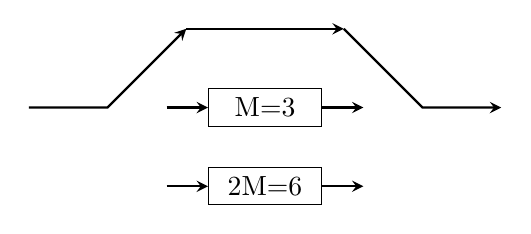
\begin{tikzpicture}[align=center]
		\node (inputM3)[draw,text width=1.2cm] at (2,0) {M=3};
		\node (inputM6)[draw,text width=1.2cm] at (2,-1) {2M=6};

		\draw [arrow] (-1,0) -- (0,0) -- (1,1);
		\draw [arrow] (1,1) -- (3,1);
		\draw [arrow] (3,1) -- (4,0) -- (5,0);
		\draw [arrow] (0.75,0) -- (inputM3.west);
		\draw [arrow] (inputM3.east) -- (3.25,0);
		\draw [arrow] (0.75,-1) -- (inputM6.west);
		\draw [arrow] (inputM6.east) -- (3.25,-1);
	\end{tikzpicture}
	\caption{M=3时卷积交织图}
	\label{fig:convolutional_interleaver}
\end{figure}
\endinput
		\begin{figure}[thb]
	\centering
	\begin{tikzpicture}[align=center]
		\node (input1)[] at (0,2) {0,3,6};
		\node (input2)[] at (0,1) {1,4,7};
		\node (input3)[] at (0,0) {2,5,8};
		\node (output1)[] at (5,2) {0};
		\node (output2)[] at (5,1) {x};
		\node (output3)[] at (5,0) {x};
		\node (M3)[draw,text width=1.5cm] at (2.5,1) {M=3};
		\node (M6)[draw,text width=1.5cm] at (2.5,0) {2M=6};
		
		\node at (5.5,2) {3};
		\node at (6,2) {6};
		\foreach \x in {6.5,7,...,9.5}{
			\node at (\x,2) {\&};
		};
		\foreach \x in {5.5,6}{
			\node at (\x,1) {x};
		};
		
		\node at (6.5,1) {1};
		\node at (7,1) {4};
		\node at (7.5,1) {7};
		\foreach \x in {8,8.5,...,9.5}{
			\node at (\x,1) {\&};
		};
		
		\foreach \x in {5.5,6,...,7.5}{
			\node at (\x,0) {x};
		};
		\node at (8,0) {2};
		\node at (8.5,0) {5};
		\node at (9,0) {8};
		\node at (9.5,0) {\&};
		
		\draw [arrow](input1) -- (output1);
		\draw [arrow](input2) -- (M3.west);
		\draw [arrow](M3.east) -- (output2);
		\draw [arrow](input3) -- (M6.west);
		\draw [arrow](M6.east) -- (output3);
		
		\foreach \x in {5.25,5.75,...,9.25}{
			\draw [arrow](\x,2.5) -- (\x,-0.5);
		};
		
		\node at (0,-1) {输入数据流};
		\node at (6,-1) {输出数据流};

	\end{tikzpicture}
	\caption{卷积交织输入输出数据结构}
	\label{fig:convolutional_interleaver_data_structure}
\end{figure}
\endinput
		\par DVB-T中使用的卷积交织,$M$=17,即第一行直通,第二行延时17字节,第三行延时2*17=34字节,以此类推,总过有12层,同步字节($\overline{\text{SYNC}}$和$\text{SYNC}_n$)总是通过第一行进行交织。
		\par 程序实现主要代码见代码\ref{code:convolutional_interleaver}。
		\begin{lstlisting}[caption = {卷积交织},label = {code:convolutional_interleaver},language = C++ ]
int dvbt_convolutional_interleaver_impl::work (int noutput_items,
				gr_vector_const_void_star &input_items,
				gr_vector_void_star &output_items)
{
	const unsigned char *in = (const unsigned char *) input_items[0];
	unsigned char *out = (unsigned char *) output_items[0];

	for (int i = 0; i < (noutput_items / d_I); i++) {
	//Process one block of I symbols
	for (unsigned int j = 0; j < d_shift.size(); j++) {
		d_shift[j]->push_front(in[(d_I * i) + j]);
		out[(d_I * i) + j] = d_shift[j]->back();
		d_shift[j]->pop_back();
	}
	}
	return noutput_items;
}
		\end{lstlisting}
	\section{内编码(卷积编码)}
		\par DVB-T系统的内编码采用卷积编码,卷积码是由$k$个信息比特编码成$n(n>k)$比特码组,编码出的l比特的码组值,不仅与当前码字中的k个信息比特值有关,而且与其前面$N-1$个码字中的$(N-1)xk$个信息比特值有关,也即当前码组内的$n$个码元,它们的值取决于$N$个码组内的全部信息码元,$N$可称为卷积码编码的约束长度。
		\par DVB-T系统可以选择几种由码率为1/2的主卷积码删余后的卷积码。无论是等级或非等级传送模式,对于某一给定业务的数据率,系统可选择最适当的码率。主码的生成多项式,对$X$路输出是$G_1=171_{OCT}$,对$Y$路输出是$G_2=133_{OCT}$。图\ref{fig:inner_coder}是主卷积码生成结构图。
		\begin{figure}[thb]
	\centering
	\begin{tikzpicture}[align=center]
		\node (and1) [] at (0,3) {$\bigoplus$};
		\node (and2) [] at (0,-3) {$\bigoplus$};
		\node (pro1) [draw,text width=3em] at (-5,0) {1比特延迟};
		\node (pro2) [draw,text width=3em] at (-3,0) {1比特延迟};
		\node (pro3) [draw,text width=3em] at (-1,0) {1比特延迟};
		\node (pro4) [draw,text width=3em] at (1,0) {1比特延迟};
		\node (pro5) [draw,text width=3em] at (3,0) {1比特延迟};
		\node (pro6) [draw,text width=3em] at (5,0) {1比特延迟};

		\draw [arrow] (-6.5,0) -- (pro1.west);
		\draw [arrow] (pro1.east) -- (pro2.west);
		\draw [arrow] (pro2.east) -- (pro3.west);
		\draw [arrow] (pro3.east) -- (pro4.west);
		\draw [arrow] (pro4.east) -- (pro5.west);
		\draw [arrow] (pro5.east) -- (pro6.west);
		\draw (pro6.east) -- (6,0);

		\draw [arrow] (-6,0) -- (-6,1) -- (-0.4,2.8);
		\draw [arrow] (-4,0) -- (-4,1) -- (-0.2,2.8);	
		\draw [arrow] (-2,0) -- (-2,1) -- (-0.1,2.8);
		\draw [arrow] (0,0) -- (0,2.8);
		\draw [arrow] (6,0) -- (6,1) -- (0.4,2.8);

		\draw [arrow] (-6,0) -- (-6,-1) -- (-0.4,-2.8);
		\draw [arrow] (-2,0) -- (-2,-1) -- (-0.2,-2.8);
		\draw [arrow] (0,0) -- (-0,-2.8);
		\draw [arrow] (4,0) -- (4,-1) -- (0.2,-2.8);
		\draw [arrow] (6,0) -- (6,-1) -- (0.1,-2.8);

		\fill (-6,0) circle (2pt);
		\fill (-4,0) circle (2pt);
		\fill (-2,0) circle (2pt);
		\fill (2,0) circle (2pt);
		\fill (4,0) circle (2pt);
		\fill (6,0) circle (2pt);


	\end{tikzpicture}
	\caption{1/2码率主卷积码}
	\label{fig:inner_coder}
\end{figure}
\endinput
		\par 除了1/2码率的主码外,系统还可以按照图\ref{fig:inner_coder_slash}使用码率为2/3,3/4,5/6,7/8的删余卷积码。
		\begin{figure}[thb]
	\centering
	\begin{tikzpicture}[align=center]
		\node (pro1) [draw,minimum width=2cm,minimum height=3cm] at (1,0) {1/2码率\\[2pt]卷积码\\[2pt]编码器};
		\node (pro2) [draw,minimum width=2cm,minimum height=3cm] at (5,0) {卷积码\\[2pt]删除};
		\node [above=3pt] at (3,1) {X};
		\node [below=3pt] at (3,-1) {Y};

		\draw [arrow] (-1,0) -- (pro1.west);
		\draw [arrow] (2,1) -- (4,1);
		\draw [arrow] (2,-1) -- (4,-1);
		\draw [arrow] (pro2.east) -- (7,0);
	\end{tikzpicture}
	\caption{1/2基本码率截取框图}
	\label{fig:inner_coder_slash}
\end{figure}
\endinput
		\par 删除卷积码的构造方法如表\ref{table:inner_coder_slash},优先发送X1。
		\begin{figure}[thb]
	\centering
	\begin{tikzpicture}[align=center]
		\node (pro1) [draw,minimum width=2cm,minimum height=3cm] at (1,0) {1/2码率\\[2pt]卷积码\\[2pt]编码器};
		\node (pro2) [draw,minimum width=2cm,minimum height=3cm] at (5,0) {卷积码\\[2pt]删除};
		\node [above=3pt] at (3,1) {X};
		\node [below=3pt] at (3,-1) {Y};

		\draw [arrow] (-1,0) -- (pro1.west);
		\draw [arrow] (2,1) -- (4,1);
		\draw [arrow] (2,-1) -- (4,-1);
		\draw [arrow] (pro2.east) -- (7,0);
	\end{tikzpicture}
	\caption{1/2基本码率截取框图}
	\label{fig:inner_coder_slash}
\end{figure}
\endinput
	\section{比特交织}
		\par DVB-T系统的内交织采用比特交织和符号交织,这两种交织都是基于块结构的。
		\par 内编码后的比特流通过解复用器后进入比特交织器,根据不同的映射模式分成$v$个子流。非等级模式下的对应关系如表\ref{table:bit_inner_interleaver_v}:
		\begin{table}[!hbp]
			\centering
			\caption{非等级模式下对应关系}
			\begin{tabular*}{5cm}{l|l}
				\hline\hline
				QPSK & $v$=2 \\
				\hline
				16QAM & $v$=4 \\
				\hline
				64QAM & $v$=6 \\
				\hline\hline
			\end{tabular*}
			\label{table:bit_inner_interleaver_v}
		\end{table}
		\par 16QAM解复用模型如图\ref{fig:bit_inner_interleaver},$x_0$映射到$b_{0,0}$,$x_1$映射到$b_{1,0}$,$x_2$映射到$b_{2,0}$,$x_3$映射到$b_{3,0}$\cite{DVB—T中内交织与解交织的算法及实现_徐翼}。
		\begin{figure}[thb]
	\centering
	\begin{tikzpicture}
		\node (demux) [draw, minimum height = 3cm, minimum width = 2cm] at (0,0) {解复用};
		\node (bit_interleaver1) [draw, minimum height = 1cm, minimum width = 3cm] at (5,3) {比特交织器I0};
		\node (bit_interleaver2) [draw, minimum height = 1cm, minimum width = 3cm] at (5,1) {比特交织器I1};
		\node (bit_interleaver3) [draw, minimum height = 1cm, minimum width = 3cm] at (5,-1) {比特交织器I2};
		\node (bit_interleaver4) [draw, minimum height = 1cm, minimum width = 3cm] at (5,-3) {比特交织器I3};

		\node at (-3,0.2) {$x_1,x_2,x_3,...$};

		\node at (2.5,3+0.2) {$b_{0,0},b_{0,1},...$};
		\node at (2.5,1+0.2) {$b_{1,0},b_{1,1},...$};
		\node at (2.5,-1+0.2) {$b_{2,0},b_{2,1},...$};
		\node at (2.5,-3+0.2) {$b_{3,0},b_{3,1},...$};

		\node at (7.5,3+0.2) {$a_{0,0},a_{0,1},...$};
		\node at (7.5,1+0.2) {$a_{1,0},a_{1,1},...$};
		\node at (7.5,-1+0.2) {$a_{2,0},a_{2,1},...$};
		\node at (7.5,-3+0.2) {$a_{3,0},a_{3,1},...$};

		\draw [arrow] (-4,0) -- (demux);
		\draw [arrow] (1,0.6) -- ++(0.3,0) -- ++(0,3-0.6) -- (bit_interleaver1.west);
		\draw [arrow] (1,0.2) -- ++(0.5,0) -- ++(0,1-0.2) -- (bit_interleaver2.west);
		\draw [arrow] (1,-0.2) -- ++(0.5,0) -- ++(0,-1+0.2) -- (bit_interleaver3.west);
		\draw [arrow] (1,-0.6) -- ++(0.3,0) -- ++(0,-3+0.6) -- (bit_interleaver4.west);
		\draw [arrow] (bit_interleaver1.east) -- ++(2,0);
		\draw [arrow] (bit_interleaver2.east) -- ++(2,0);
		\draw [arrow] (bit_interleaver3.east) -- ++(2,0);
		\draw [arrow] (bit_interleaver4.east) -- ++(2,0);
	\end{tikzpicture}
	\caption{比特内交织原理图}
	\label{fig:bit_inner_interleaver}
\end{figure}
\endinput
		\par 比特交织仅在有用的数据上进行,比特交织块的大小为126字节,在2K模式下每个OFDM符号中的有效数据在交织过程中重复12次,8K模式下需要重复48次。每一路比特交织器,输入的比特向量定义为:
		\begin{equation}
			B(e)=(b_{e,0},b_{e,1},b_{e,2},\cdots b_{e,125}),e\in[0,v-1]
		\end{equation}
		\par 交织后的输出向量定义为:
		\begin{equation}
			A(e)=(a_{e,0},a_{e,1},a_{e,2},\cdots a_{e,125}),e\in[0,v-1]
		\end{equation}
		\par 则:
		\begin{equation}
			a_{e,w}=b_{e,He(w)},w\in[0,125]
		\end{equation}
		\par $He_{w}$为一置换函数,对于每一路交织器置换函数$He_{w}$均不相同,$He_{w}$定义如表\ref{table:inner_interleaver_hew}。以交织器I3为例,$w$为输入数据地址,$H(w)$为输出数据地址,即先将输入数据输入到126个地址空间中,输出时先输出地址42~125中的数据,在输出地址0~41中的数据。
		\begin{table}[!h]
	\centering
	\caption{比特交织器置换函数}
	\begin{tabular}{|l|l|}
	\hline
	\multicolumn{1}{|c|}{比特交织器} & \multicolumn{1}{|c|}{置换函数} \\
	\hline
	I0 & $H0(w)=w$ \\
	\hline
	I1 & $H1(w)=(w+63) mod 126$ \\
	\hline
	I2 & $H1(w)=(w+105) mod 126$ \\
	\hline
	I3 & $H1(w)=(w+42) mod 126$ \\
	\hline
	I4 & $H1(w)=(w+21) mod 126$ \\
	\hline
	I5 & $H1(w)=(w+84) mod 126$ \\
	\hline
	\end{tabular}
	\label{table:inner_interleaver_hew}
\end{table}

\endinput
		\par $v$比特交织器的输出共同组成了一个$v$比特数据字。因此,整个比特交织器的输出是一个$v$比特字$y'$,其中I0支路的输出为最高位。
		\begin{equation}
			y_w'=(a_{0,w},a_{1,w},a_{2,w},\cdots a_{v-1,w},),w\in[0,125],v\in[1,6]
		\end{equation}
		\par 程序实现主要代码见代码\ref{code:bit_inner_interleaver}。
		\begin{lstlisting}[caption = {比特内交织}, label = {code:bit_inner_interleaver}, language = C++ ]
int dvbt_bit_inner_interleaver_impl::general_work (int noutput_items,
			gr_vector_int &ninput_items,
			gr_vector_const_void_star &input_items,
			gr_vector_void_star &output_items)
{
	const unsigned char *inh = (const unsigned char *) input_items[0];
	const unsigned char *inl = (const unsigned char *) input_items[1];
	unsigned char *out = (unsigned char *) output_items[0];

	int bmax = noutput_items * d_nsize / d_bsize;

	// First index of d_b is Bit interleaver number
	// Second index of d_b is the position inside the Bit interleaver
	unsigned char d_b[MAX_MODULATION_ORDER][INTERLEAVER_BLOCK_SIZE];

	for (int bcount = 0; bcount < bmax; bcount++) {
	for (int i = 0; i < d_bsize; i++) {
		if (d_hierarchy == NH) {
		int c = inh[bcount * d_bsize + i];

		// Create the demultiplexer
		for (int k = 0; k < d_v; k++) {
			d_b[d_perm[(d_v * i) + k]][i] = (c >> (d_v - k - 1)) & 1;
		}
		}
		else {
		int ch = inh[(bcount * d_bsize) + i];
		int cl = inl[(bcount * d_bsize) + i];

		// High priority input - first 2 streams
		for (int k = 0; k < 2; k++) {
			d_b[(d_v * i + k) % 2][(d_v * i + k) / 2] = (ch >> (1 - k)) & 1;
		}

		// Low priority input - (v - 2) streams
		for (int k = 2; k < (d_v - 2); k++) {
			d_b[d_perm[d_v * i + k]][(d_v * i + k) / (d_v - 2)] = (cl >> (d_v - k - 1)) & 1;
		}
		}
	}

	// Take one bit from each interleaver
	// and format the output

	for (int w = 0; w < d_bsize; w++) {
		int val = 0;

		for (int e = 0; e < d_v; e++) {
		val = (val << 1) | d_b[e][H(e, w)];
		}

		out[(bcount * d_bsize) + w] = val;
	}
	}

	// Tell runtime system how many input items we consumed on
	// each input stream.
	consume_each (noutput_items);

	// Tell runtime system how many output items we produced.
	return noutput_items;
}
		\end{lstlisting}
	\section{符号交织}
		\par 符号交织用于将$v$比特字映射到每个OFDM的有效载波上,其中2K模式下为1512个有效载波,8K模式下为6048个有效载波。
		\par 首先将比特交织输出的$N_{max}$个$v$比特字(2K模式下为$12*126=1512$个,8K模式下为$48*126=6048$个)顺序写入矢量$Y^{in}=(y_0^{in},y_1^{in},y_2^{in},\cdots,y_{N_{max}-1}^{in})$中,接下来对该矢量进行交织,其中2K模式下$N_{max}=1512$,8K模式下$N_{max}=6048$。经过交织后的矢量$Y^{out}=(y_0^{out},y_1^{out},y_2^{out},\cdots,y_{N_{max}-1}^{out})$定义为:
		\par OFDM帧中的偶数符号:
		\begin{equation}
			y_{H(q)}^{out}=y_q^{in}
		\end{equation}
		\par OFDM帧中的奇数符号:
		\begin{equation}
			y_q^{out}=y_{H(q)}^{in}
		\end{equation}
		\par 其中$H(q)$是DVB-T标准中定义的一个专门的置换函数。首先定义一个$N_r-1$位的二进制数$R'_i$,其中$N_r=\log_{2}M_{max}$(2K模式下$M_{max}=2048$,8K模式下$M_{max}=8192$),$R'_i$符号下面的规定:
		\begin{equation}
			\begin{array}{ll}
				R'_i[N_r-2,N_r-3,\cdots,1,0]=0,0,\cdots,0,0                                                                       & i={0,1}     \\
				R'_i[N_r-2,N_r-3,\cdots,1,0]=0,0,\cdots,0,1                                                                       & i=2         \\
				\{R'_i[N_r-3,N_r-4,\cdots,1,0]=R'_i[N_r-2,N_r-3,\cdots,2,1]                                                       & 2<i<M_{max} \\
				\quad\quad 2K\text{模式}:R'_i[9]=R'_{i-1}[0]\bigoplus R'_{i-1}[3]                                               &             \\
				\quad\quad 8K\text{模式}:R'_i[11]=R'_{i-1}[0]\bigoplus R'_{i-1}[1]\bigoplus R'_{i-1}[4]\bigoplus R'_{i-1}[46]\} &             \\
			\end{array}
		\end{equation}
		\par 再定义一个矢量$R_i$,矢量$R_i$由$R'_i$按如表\ref{table:symbol_interleaver_bit_replace}的要求置换得到\cite{DVB—T中内交织与解交织的算法及实现_徐翼}。
		\begin{table}[!hbp]
	\centering
	\caption{符号交织比特置换}
	\begin{tabular}{|c|c|c|c|c|c|c|c|c|c|c|c|c|}
	\hline\hline
	\multicolumn{13}{|c|}{2K模式} \\
	\hline
	\multicolumn{3}{|c|}{$R'_i$的比特位置} & 9 & 8 & 7 & 6 & 5 & 4 & 3 & 2 & 1 & 0 \\
	\hline
	\multicolumn{3}{|c|}{$R_i$的比特位置} & 0 & 7 & 5 & 1 & 8 & 2 & 6 & 9 & 3 & 4 \\
	\hline
	\multicolumn{13}{|c|}{8K模式} \\
	\hline
	$R'_i$的比特位置 & 11 & 10 & 9 & 8 & 7 & 6 & 5 & 4 & 3 & 2 & 1 & 0 \\
	\hline
	$R'_i$的比特位置 & 5 & 11 & 3 & 0 & 10 & 8 & 6 & 9 & 2 & 4 & 1 & 7 \\
	\hline\hline
	\end{tabular}
	\label{table:symbol_interleaver_bit_replace}
\end{table}

\endinput
		\par 则$H(q)$符合以下算法:
		\par\noindent $q=0;$
		\par\noindent $for\quad (i=0;i<M_{max};i++)\{$
		\par\noindent $\qquad H(q)=(i\quad mod\quad 2)\cdot 2^{N_r-1}+\Sigma_{j=0}^{N_r-2}R_i(j)\cdot 2^j;$
		\par\noindent $\qquad if(H(q)<N_{max})$
		\par\noindent $\qquad\qquad q=q+1;$
		\par\noindent $\}$
		\par 本部分程序段过长,参见\href{https://github.com/gnuradio/gnuradio/blob/master/gr-dtv/lib/dvbt/dvbt_symbol_inner_interleaver_impl.cc}{https://github.com/gnuradio/gnuradio/blob/master/gr-dtv/lib/dvbt/dvbt\_symbol\_inner\_interleaver\_impl.cc}
	\section{星座映射}
		\par DVB-T系统采用正交频分复用传输(OFDM)传输,一个OFDM帧的所有数据载波调制采用格雷(Grey)映射的QPSK、16QAM、64QAM、非均匀16QAM或非均匀64QAM映射为复数Z。本设计采用16QAM均匀模式,其星座图如图\ref{fig:dvbt_map_16QAM}。
		\begin{figure}[thb]
	\centering
	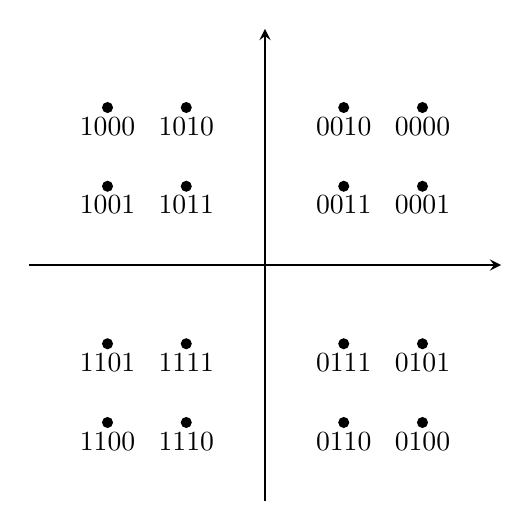
\begin{tikzpicture}
		\fill (1,1) circle (2pt) node [below] {0011};
		\fill (1,2) circle (2pt) node [below] {0010};
		\fill (2,1) circle (2pt) node [below] {0001};
		\fill (2,2) circle (2pt) node [below] {0000};
		\fill (-1,1) circle (2pt) node [below] {1011};
		\fill (-1,2) circle (2pt) node [below] {1010};
		\fill (-2,1) circle (2pt) node [below] {1001};
		\fill (-2,2) circle (2pt) node [below] {1000};
		\fill (-1,-1) circle (2pt) node [below] {1111};
		\fill (-1,-2) circle (2pt) node [below] {1110};
		\fill (-2,-1) circle (2pt) node [below] {1101};
		\fill (-2,-2) circle (2pt) node [below] {1100};
		\fill (1,-1) circle (2pt) node [below] {0111};
		\fill (1,-2) circle (2pt) node [below] {0110};
		\fill (2,-1) circle (2pt) node [below] {0101};
		\fill (2,-2) circle (2pt) node [below] {0100};
		\draw [arrow] (-3,0) -- (3,0);
		\draw [arrow] (0,-3) -- (0,3);
	\end{tikzpicture}
	\caption{16QAM星座映射}
	\label{fig:dvbt_map_16QAM}
\end{figure}
\endinput
		\par 其他模式星座图与之类似。
		\par 程序实现主要代码见代码\ref{code:dvbt_map}。
		\begin{lstlisting}[caption = {星座映射},label = {code:dvbt_map}, language = C++ ]
void dvbt_map_impl::make_constellation_points(int size, int step, int alpha)
{
	// The symmetry of the constellation is used to calculate
	// 16-QAM from QPSK and 64-QAM form 16-QAM

	int bits_per_axis = log2(size) / 2;
	int steps_per_axis = sqrt(size) / 2 - 1;

	for (int i = 0; i < size; i++) {
	// This is the quadrant made of the first two bits starting from MSB
	int q = i >> (2 * (bits_per_axis - 1)) & 3;
	// Sign for correctly calculate I and Q in each quadrant
	int sign0 = (q >> 1) ? -1 : 1; int sign1 = (q & 1) ? -1 : 1;

	int x = (i >> (bits_per_axis - 1)) & ((1 << (bits_per_axis - 1)) - 1);
	int y = i & ((1 << (bits_per_axis - 1)) - 1);

	int xval = alpha + (steps_per_axis - x) * step;
	int yval = alpha + (steps_per_axis - y) * step;

	int val = (bin_to_gray(x) << (bits_per_axis - 1)) + bin_to_gray(y);

	// ETSI EN 300 744 Clause 4.3.5
	// Actually the constellation is gray coded
	// but the bits on each axis are not taken in consecutive order
	// So we need to convert from b0b2b4b1b3b5->b0b1b2b3b4b5(QAM64)

	x = 0; y = 0;

	for (int j = 0; j < (bits_per_axis - 1); j++) {
		x += ((val >> (1 + 2 * j)) & 1) << j;
		y += ((val >> (2 * j)) & 1) << j;
	}

	val = (q << 2 * (bits_per_axis - 1)) + (x << (bits_per_axis - 1)) + y;

	// Keep corresponding symbol bits->complex symbol in one vector
	// Normalize the signal using gain
	d_constellation_points[val] = d_gain * gr_complex(sign0 * xval, sign1 * yval);
	}
}
		\end{lstlisting}
	\section{参考信号}
		\par DVB-T系统中2K模式和8K模式分别含有1705和6817个子载波,这些子载波的作用可以分为三类:
		\par (1)数据载波,负责传递MPEG-2 TS流信号。
		\par (2)传输参数信令载波(TPS: Transport Parameter Signaling)含有方便接收终端接收信号的所需的参数,例如:调制方式(QPSK,16QAM,64QAM),信号纠错码(1/2,2/3,3/4,5/6,7/8),2k和8k模式,保护间隔(1/4,1/8,1/16,1/32)等。
		\par (3) 导频信号载波(Pilot),用来帮助接收机对信号幅度及相位进行预估及校正,改善接收质量。
		\par 在有效载波数的基础上,通常会加入一些虚拟载波使其载波总数达到2的n次方,例如加入虚拟载波以后8k模式的总载波数量为8192,是2的13次方,2k模式的总载波数量为2048,是2的11次方,以方便计算机采用反向快速富里叶变换,这也是2k和8k模式名称的由来。在接收机端,通过采用快速富里叶变换,机顶盒可以解调出2k或8k的COFDM信号\cite{DVB—T编码调制的仿真和FPGA实现_王闯}。
		\par 即:
		\par 2K模式:
		\par 总载波数量1705=1512(数据)+17(传输参数信令)+176(导频)
		\par 8K模式:
		\par 总载波数量6817=7048(数据)+68(传输参数信令)+701(导频)
		\par 传数参数信令(TPS)是为了方便机顶盒的信道解码而发送的传输参数,对于2k模式TPS占用17个载波,对于8k模式TPS占用68个载波,它们所占用的载波序号见表\ref{table:tps_carrier},它们所传输的信息是:调制方式,等级调制信息,保护间隔,纠错保护码,传输模式,超级帧中的帧序号,发射机所覆盖的蜂窝标识,等,详细含义见表\ref{table:tps}。
		\begin{table}[!htbp]
	\centering
	\caption{TPS载波序号位置}
	\begin{tabular}{|p{5cm}|p{5cm}|}
	\hline\hline
	\multicolumn{1}{|c|}{2K模式TPS载波的位置} & \multicolumn{1}{c|}{8K模式TPS载波的位置} \\
	\hline
	34,50,209,346,413,569,595,688,790,901,1073,1219,1262,1286,1469,1594,1687 & 34,50,209,346,413,569,595,688,790,901,1073,1219,1262,1286,1469,1594,1687,1738,1754,1913,2050,2117,2273,2299,2392,2494,2605,2777,2923,2966,2990,3173,3298,3391,3442,3458,3617,3754,3821,3977,4003,4096,4198,4309,4481,4627,4670,4694,4877,5002,5095,
5146,5162,5321,5458,5525,5681,5707,5800,5902,6013,6185,6331,6374,6398,6581,6706,6799 \\
	\hline\hline
	\end{tabular}
	\label{table:tps_carrier}
\end{table}

\endinput
		\begin{table}[!htbp]
	\centering
	\caption{TPS信息内容定义}
	\begin{tabular}{|m{2cm}<{\centering}|m{3cm}<{\centering}|m{8cm}<{\centering}|}
	\hline\hline
	\multicolumn{1}{|c|}{TPS比特序号} & \multicolumn{1}{c|}{数据含义} & \multicolumn{1}{c|}{数据格式} \\
	\hline
	$S_0$ & 初始位 & BPSK调制初始位,它是从PRBS随机序列发生器生成 \\
	\hline
	$S_1-S_{16}$ & 同步字 & \tabincell{c}{0011010111101110 \\ 或 \\ 1100101000010001} \\
	\hline
	$S_{17}-S_{22}$ & TPS长度指示 & \tabincell{l}{010111 如果不采用覆盖区域蜂窝号码 \\ 011111 如果采用覆盖区域蜂窝号码}\\
	\hline
	$S_{23},S_{24}$ & 帧序号 & \tabincell{l}{00:超级帧的第一帧 \\ 01:超级帧的第二帧 \\ 10:超级帧的第三帧 \\ 11:超级帧的第四帧} \\
	\hline
	$S_{25},S_{s6}$ & 调制方式 & \tabincell{l}{00:QPSK \\ 01:16QAM \\ 10:64QAM \\ 11:未定义} \\
	\hline
	$S_{27},S_{28},S_{29}$ & 等级调制信息 & \tabincell{l}{000:非等级调制 \\ 001:等级调制,Alpha=1 \\ 011:等级调制,Alpha=2 \\ 011:等级调制,Alpha=4 \\ 100,101,110,111:未定义} \\
	\hline
	$S_{30},S_{31},S_{32}$ & 高优先级等级调制FEC纠错码 & \tabincell{c}{000:1/2 \qquad 001:2/3 \\ 011:3/4 \qquad 011:5/6 \\ 100:7/8 \\ 101,110,111:未定义} \\
	\hline
	$S_{33},S_{34},S_{35}$ & 低优先级等级调制FEC纠错码 & \tabincell{c}{000:1/2 \qquad 001:2/3 \\ 011:3/4 \qquad 011:5/6 \\ 100:7/8 \\ 101,110,111:未定义} \\
	\hline
	$S_{36},S_{37}$ & 保护间隔 & \tabincell{l}{00:1/32 \\ 01:1/16 \\ 10:1/8 \\ 11:1/4} \\
	\hline
	$S_{38},S_{39}$ & 传输模式 & \tabincell{c}{00:2k \qquad 01:8k \\ 10,11:未定义} \\
	\hline
	$S_{40}-S_{47}$ & 覆盖区域蜂窝号码 & \tabincell{l}{当传输第1和第3帧时,\\对应蜂窝号码Cell\_ID15-8高比特序号; \\ 当传输第2和第4帧时,\\对应蜂窝号码Cell\_ID7-0低比特序号} \\
	\hline
	$S_{48}-S_{53}$ & 今后使用 & 全部设置为零 \\
	\hline
	$S_{54}-S_{67}$ & 纠错保护码 & BCH编码 \\
	\hline\hline
	\end{tabular}
	\label{table:tps}
\end{table}

\endinput
		\par 值得注意的是TPS信号既不是采用QPSK,也不是采用16QAM和64QAM的调制方式,而是采用比它们都更加抗干扰的BPSK调制,接收TPS信号的门限比QPSK还要低,机顶盒可以接收到TPS信号,未必可以接到数字电视信号。
		\par 本部分程序段过长,参见\href{https://github.com/gnuradio/gnuradio/blob/master/gr-dtv/lib/dvbt/dvbt\_reference\_signals\_impl.cc}{https://github.com/gnuradio/gnuradio/blob/master/gr-dtv/lib/dvbt/dvbt\_reference\_signals\_impl.cc}
	\section{IFFT}
		\par 傅里叶变换是将时域和频域联系起来的工具,将信号的时域表示用频域表示出来,傅里叶变换能够直接计算出给定时域信号在频域上的表示,反傅里叶变换为其逆过程,能够算出给定频域信号在时域的表示。
		\par 忽一人大呼“火起”,夫起大呼,妇亦起大呼。两儿齐哭。俄而百千人大呼,百千儿哭,百千犬吠。中间力拉崩倒之声,火爆声,呼呼风声,百千齐作;又夹百千求救声,曳屋许许声,抢夺声,泼水声。凡所应有,无所不有。虽人有百手,手有百指,不能指其一端;人有百口,口有百舌,不能名其一处也。傅里叶变换指其各端,名其处处\cite{zhihu:如何直观形象、生动有趣地给文科学生介绍傅立叶变换?}。
		\par OFDM的理论很久以前就提出来了,但是一直没有好的实现方式,因为需要计算出各个信号在时域上的叠加很困难,直到快速傅里叶变换的出现,大大降低了傅里叶变换的复杂度,能够很快地计算出信号在时域上的叠加以后的结果,使得OFDM的广泛使用成为可能。
		\par IFFT模块的功能相当于说:别麻烦发送N个子载波信号了,我直接算出你们在空中会叠加成啥样子吧;FFT模块的功能相当于说:别用老式的积分方法来去除其余的正交子载波了,我帮你一次把N个携带信号全算出来吧。就是这样,IFFT实现OFDM的系统用"数学的方法",在发送端计算信号的叠加波形,在接收端去除正交子载波,从而大大简化了系统的复杂度\cite{给"小白"图示讲解OFDM的原理}。
		\par DVB-T发射系统中采反傅里叶变换,将频域信号的在时域上叠加后的结果一次性计算出来,再在接收端使用傅里叶变换进行还原。
		\par 由于FFT已经有了众多的实现方式,此处不提供代码。
	% \section{OFDM循环前缀}
		% TODO:OFDM循环前缀
	% 	\par 在传播过程中如果子载波的正交性遭到破环,会影响信号接收,造成信道间干扰(ICI),为了克服这种干扰,OFDM传播系统采取添加循环前缀的措施来减少信道间干扰。
		% \section{常数}
		% \section{重采样}
		% 	\par 信号的采样率,用于满足另一个系统的要求
	\section{USRP发射}
		% TODO: 图片、参数
		\par 

% %!TEX root = ../paper.tex
\chapter{DVB-T接收端}
\section{USRP接收、信号源}
\section{重采样}
\section{乘常数}
\section{OFDM符号查询}
\section{FFT}
\section{解参考信号}
\section{星座解映射}
\section{符号解交织}
\section{比特内解交织}
\section{矢量串流}
\section{维特比解码}
汇编加速
\section{卷积解交织}
\section{RS解码}
\section{能量解扩散}
\section{文件输出}
% \endinput
%!TEX root = ../paper.tex
\chapter{GNU Radio实现}
	\section{GNU Radio框图}
		\par 按照图\ref{fig:gnuradio_dvbt_tx}在GNU Radio中搭建DVB-T发射端,图\ref{fig:gnuradio_dvbt_rx}在GNU Radio中搭建DVB-T接收端。
		\par 在右侧的模块中选择相应模块,使用Ctrl+f快捷键能更快的找到相应的模块。
		\begin{figure}[htb]
			\centering
			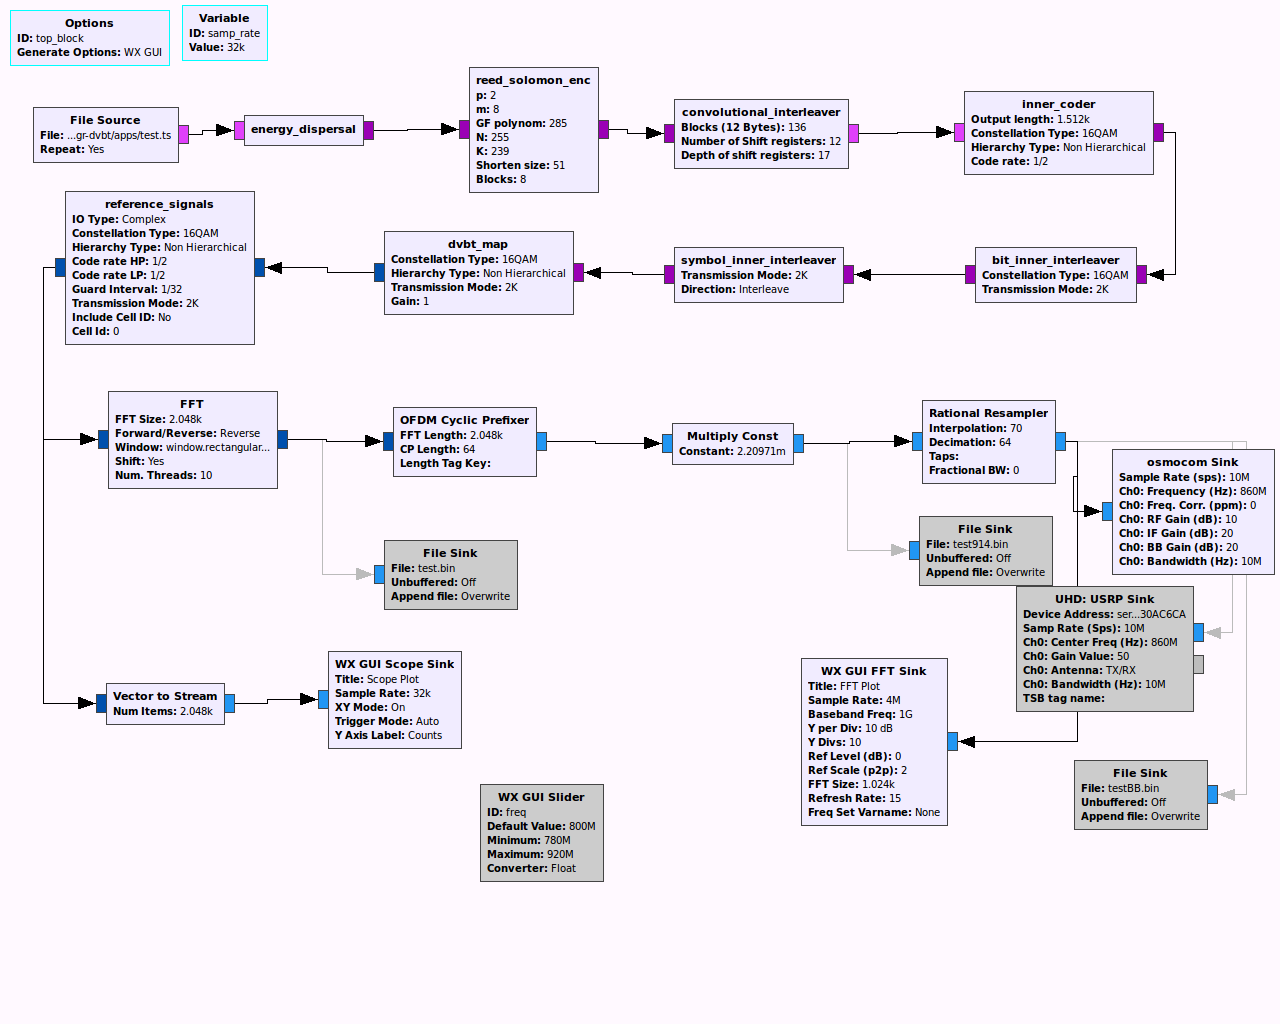
\includegraphics[height=13cm,angle=-90]{figures/dvbt_tx.png}
			\caption{GNU Radio DVB-T发射端}
			\label{fig:gnuradio_dvbt_tx}
		\end{figure}
		\begin{figure}[htb]
			\centering
			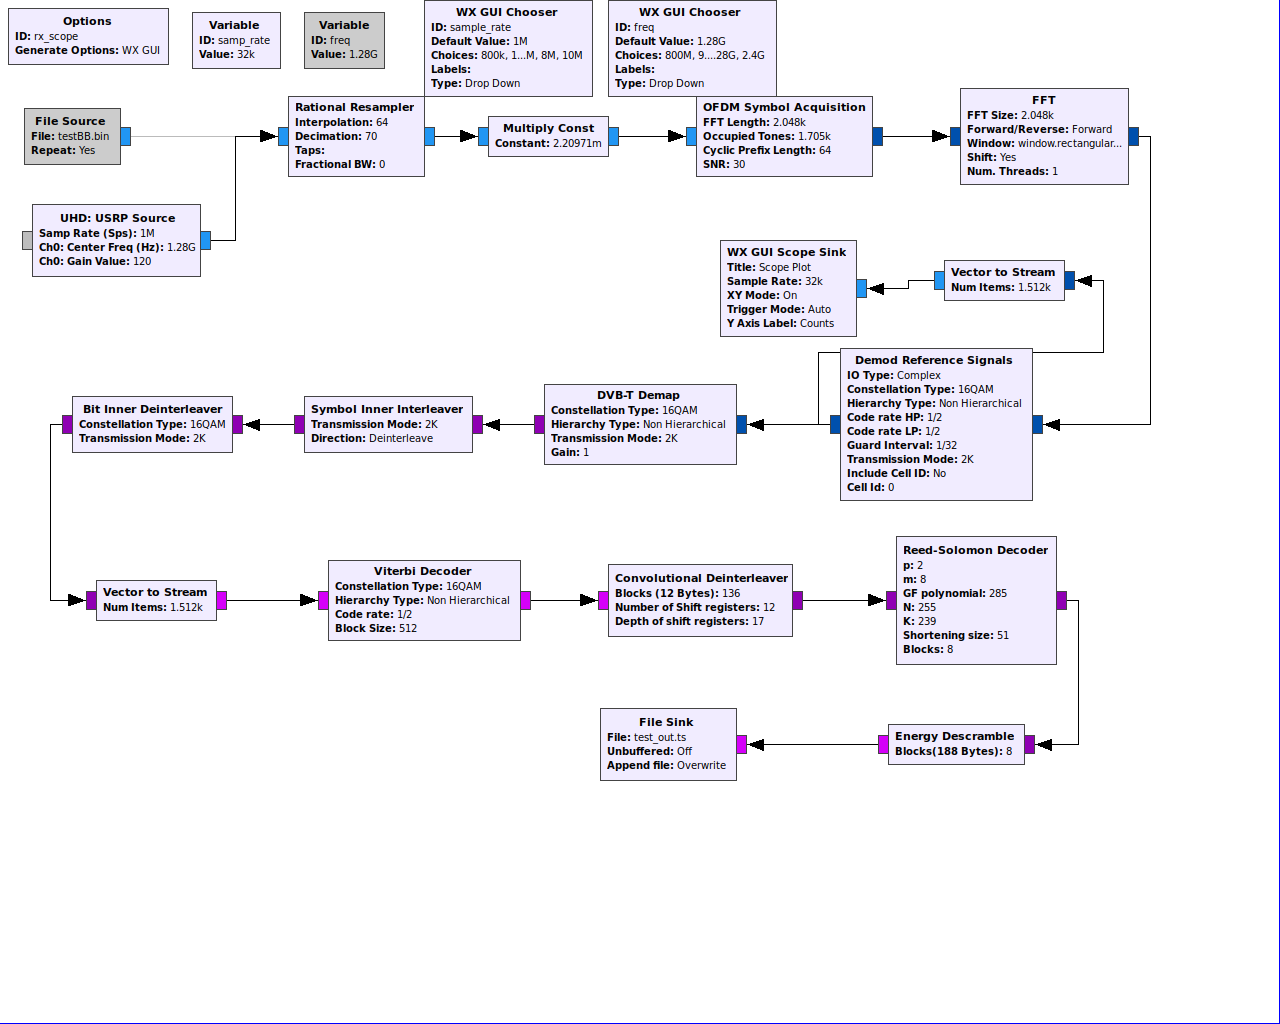
\includegraphics[height=13cm,angle=-90]{figures/dvbt_rx.png}
			\caption{GNU Radio DVB-T接收端}
			\label{fig:gnuradio_dvbt_rx}
		\end{figure}
	\section{设备连接}
		% TODO:图片标注
		\par 按图\ref{fig:devices}将设备连接,需要将USRP连接至USB3.0上,因为USB2.0的传输速率为8MS/s @ 16-bit I/Q,USB3.0的传输速率为61.44MS/s @ 16-bit I/Q\cite{USRP:SamplingRates}。
		\begin{figure}[htp]
			\centering
			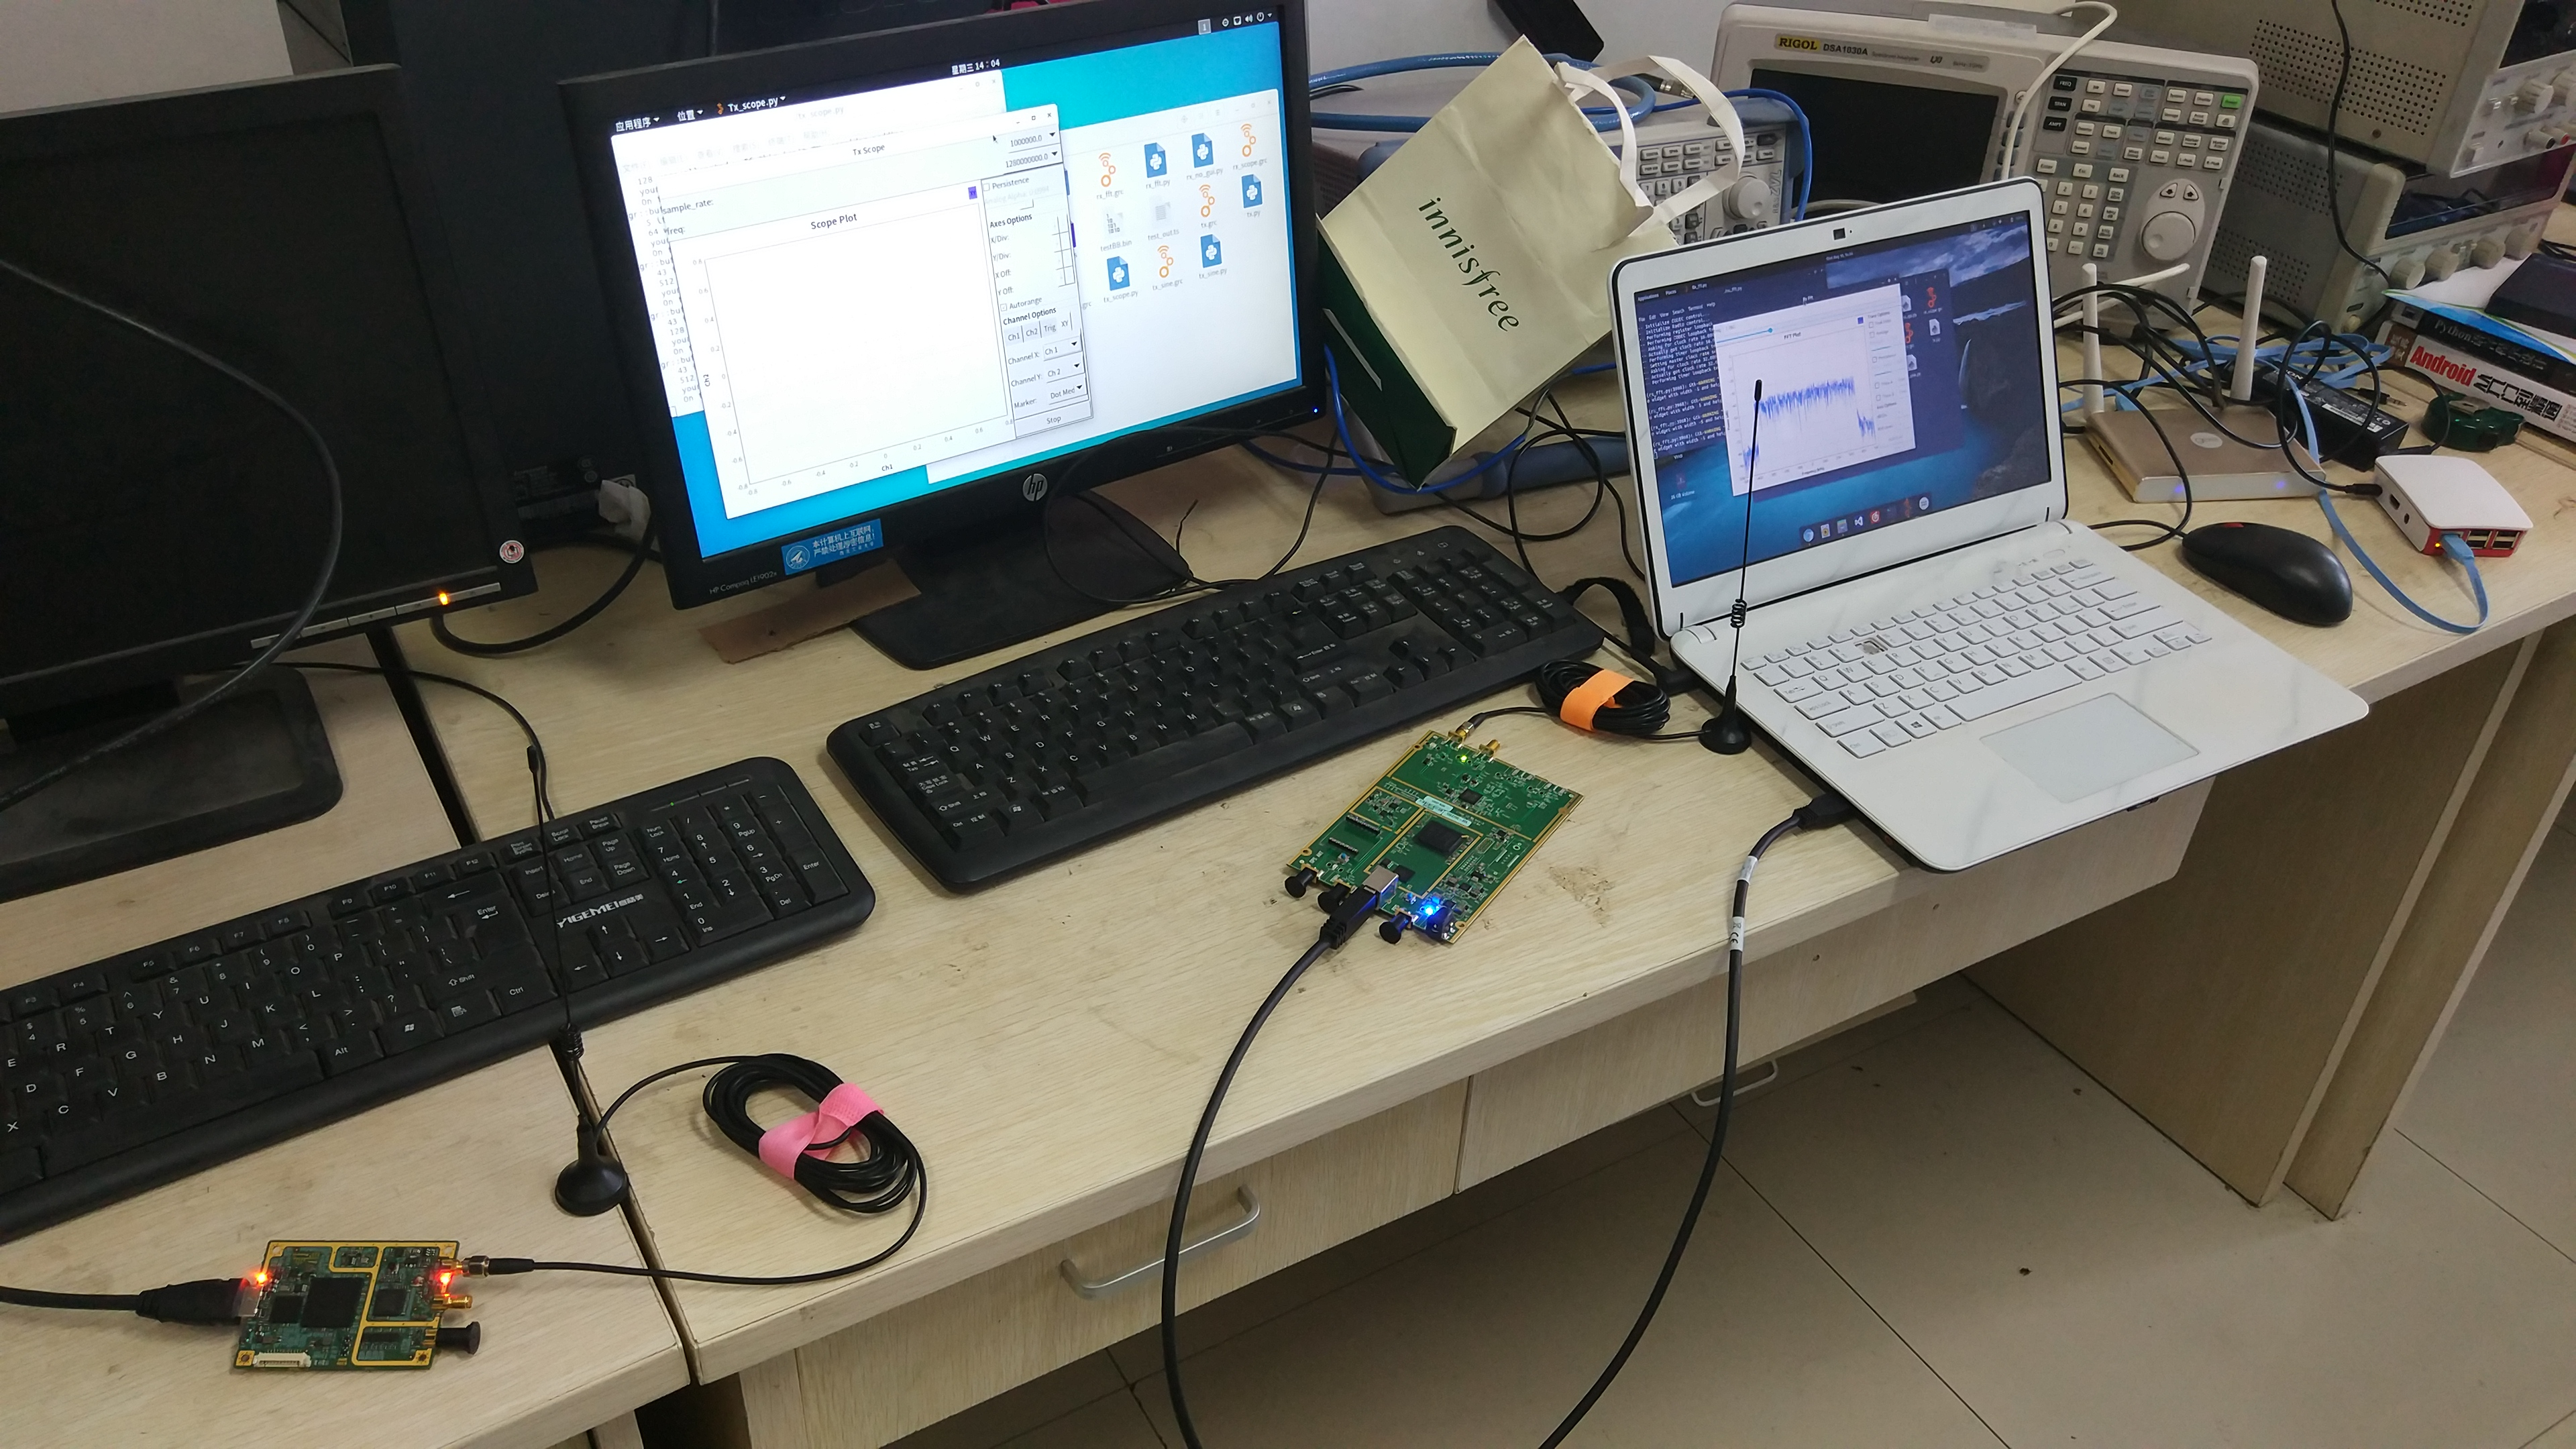
\includegraphics[width=13cm]{figures/devices.jpg}
			\caption{设备连接}
			\label{fig:devices}
		\end{figure}
	\section{运行程序}
		\par 点击GNU Radio中的运行(Run)按钮如图\ref{fig:dvbt_run},会在当前界面中直接运行该程序,直接运行可能会提示\lstinline[language=sh]{file not found}的错误,此时需要在\lstinline[language=sh]{file source}框图中指定文件的绝对位置,生成Python文件则只需要在同一目录下即可。
		\par 点击GNU Radio上的生成(Generate)按钮如图\ref{fig:dvbt_generate},会成成一个于Options框图中ID相对应的Python文件(默认为\lstinline[language=sh]{top_block.py}),进入该文件所在目录,执行:
		\begin{figure}[htp]
			\centering
			\subfigure[在当前界面中运行]{%
				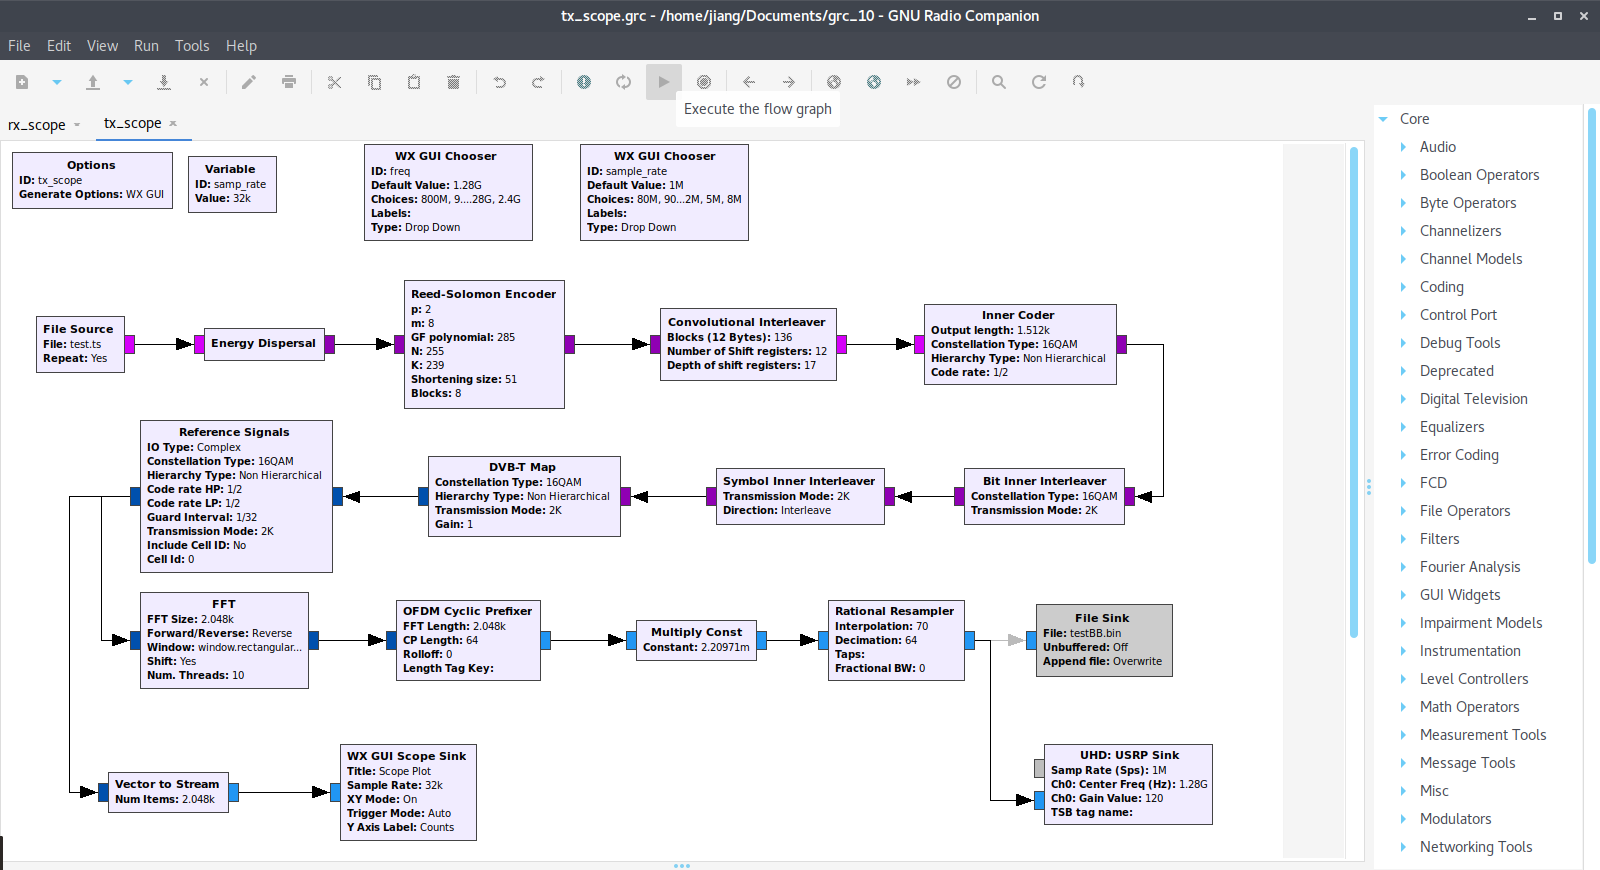
\includegraphics[width=0.4\textwidth]{figures/dvbt_run.png}
				\label{fig:dvbt_run}}
			\subfigure[生成Python文件]{%
				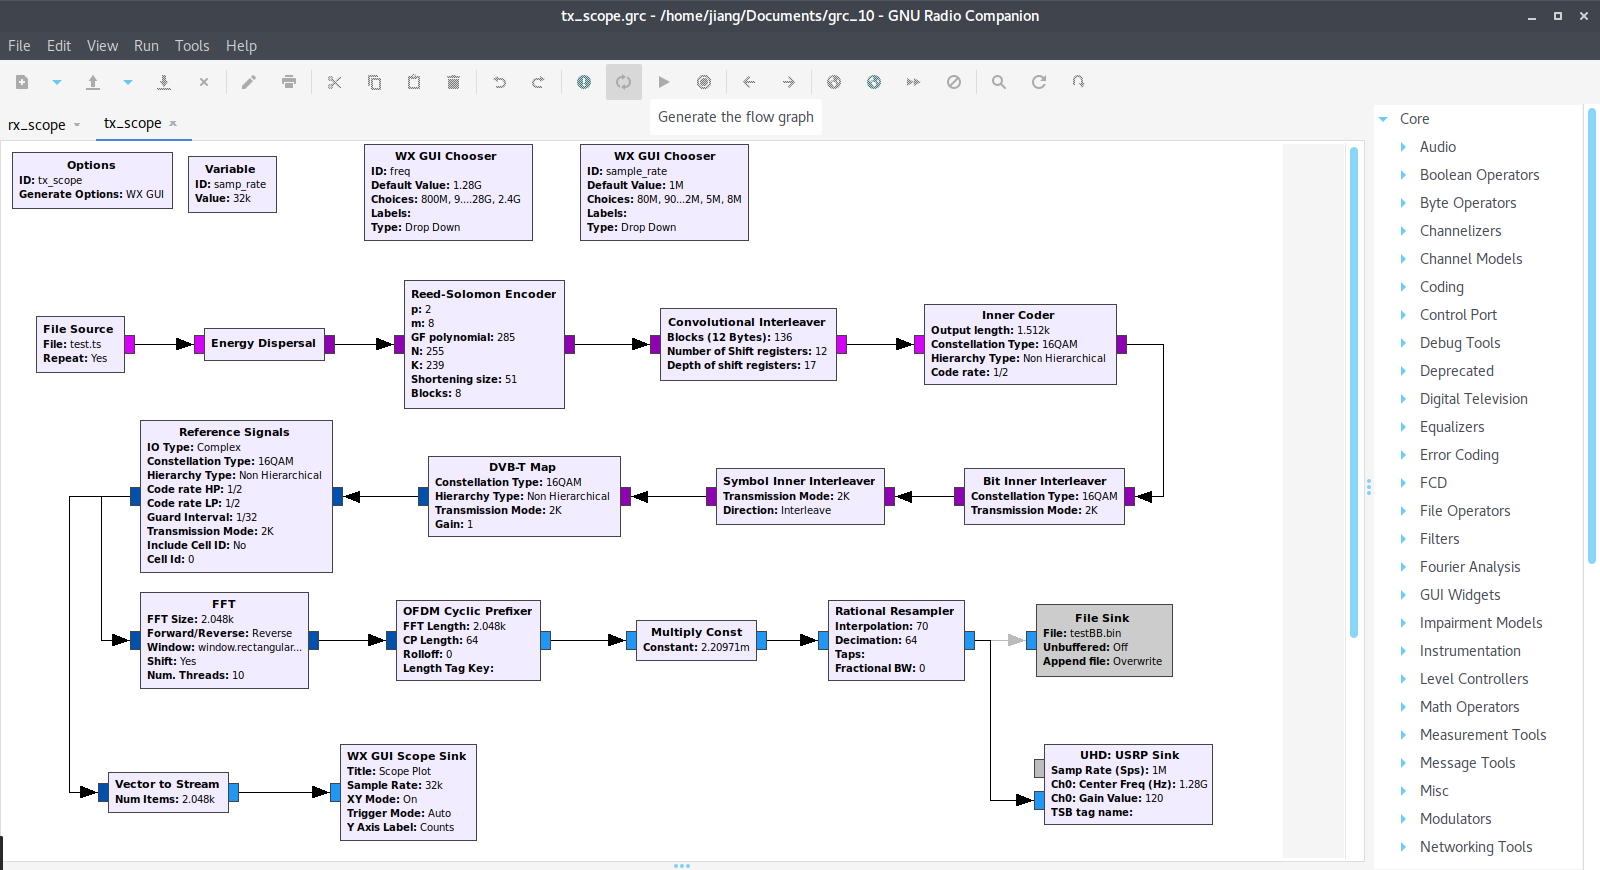
\includegraphics[width=0.4\textwidth]{figures/dvbt_generate.png}
				\label{fig:dvbt_generate}} \\
		\end{figure}
		\begin{lstlisting}[ language = sh ]
python top_block.py
		\end{lstlisting}
		\par 将其中的\lstinline[language=sh]{top_block.py}改为与之对应的文件名,如果出现\lstinline[language=sh]{no module named gnuradio}是因为当前的运行环境为Python3,则执行以下命令:
		\begin{lstlisting}[ language = sh ]
python2.7 top_block.py
		\end{lstlisting}
		\par 出现如图\ref{fig:dvbt_runtime},即表示正常运行。
		\begin{figure}[htp]
			\centering
			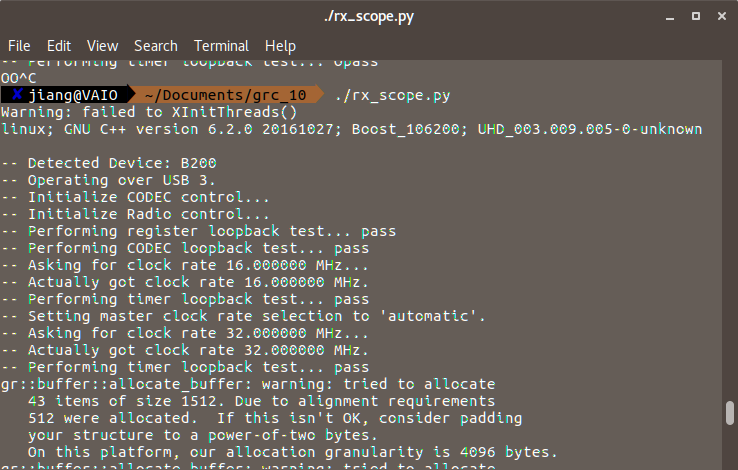
\includegraphics[width=13cm]{figures/dvbt_runtime.png}
			\caption{运行程序}
			\label{fig:dvbt_runtime}
		\end{figure}
		
				

%!TEX root = ../paper.tex
\chapter{程序运行效果}
	\section{星座图}
		\par 在电脑上,如果程序正常运行,则可以在接收端看到如图\ref{fig:dvbt_rx_map_1}和\ref{fig:dvbt_rx_map_2}星座图。
		\begin{figure}[htp]
			\centering
			\subfigure[DVB-T接收端星座图]{%
				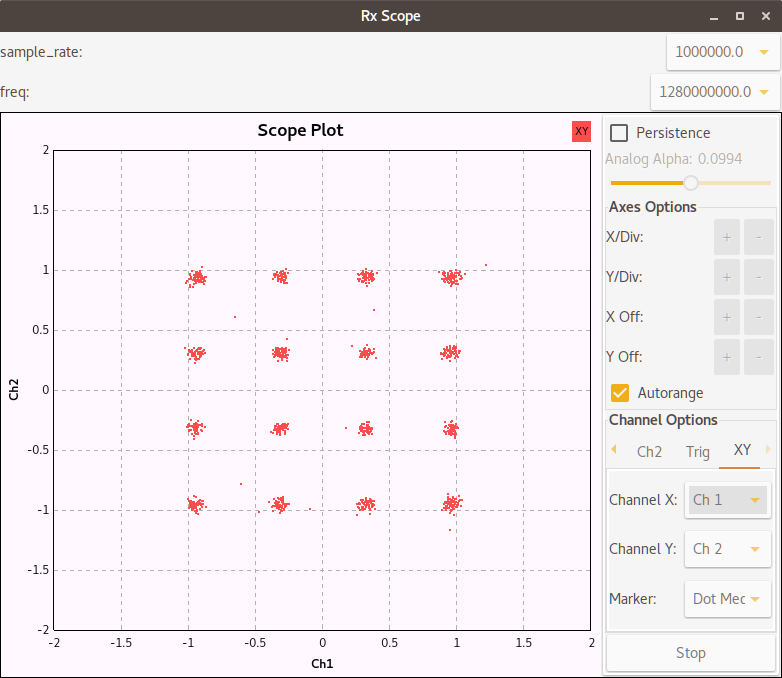
\includegraphics[width=0.4\textwidth]{figures/dvbt_rx_map_1.png}
				\label{fig:dvbt_rx_map_1}}
			\subfigure[DVB-T接收端星座图]{%
				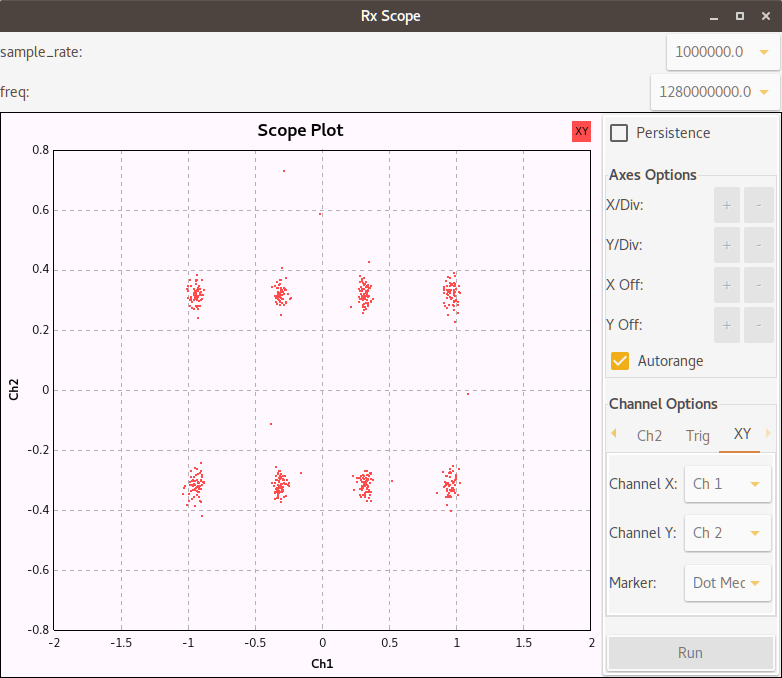
\includegraphics[width=0.4\textwidth]{figures/dvbt_rx_map_2.png}
				\label{fig:dvbt_rx_map_2}} \\
		\end{figure}
	\section{波形}
		\par 有如下几种方式查看输出波形:
		\par $\bullet$ 使用GNU Radio构建一个简易的示波器。
		\par 按图搭建框图\ref{fig:dvbt_rx_fft}运行即可,其效果如图\ref{fig:dvbt_rx_fft_1}所示。
		\begin{figure}[htp]
			\centering
			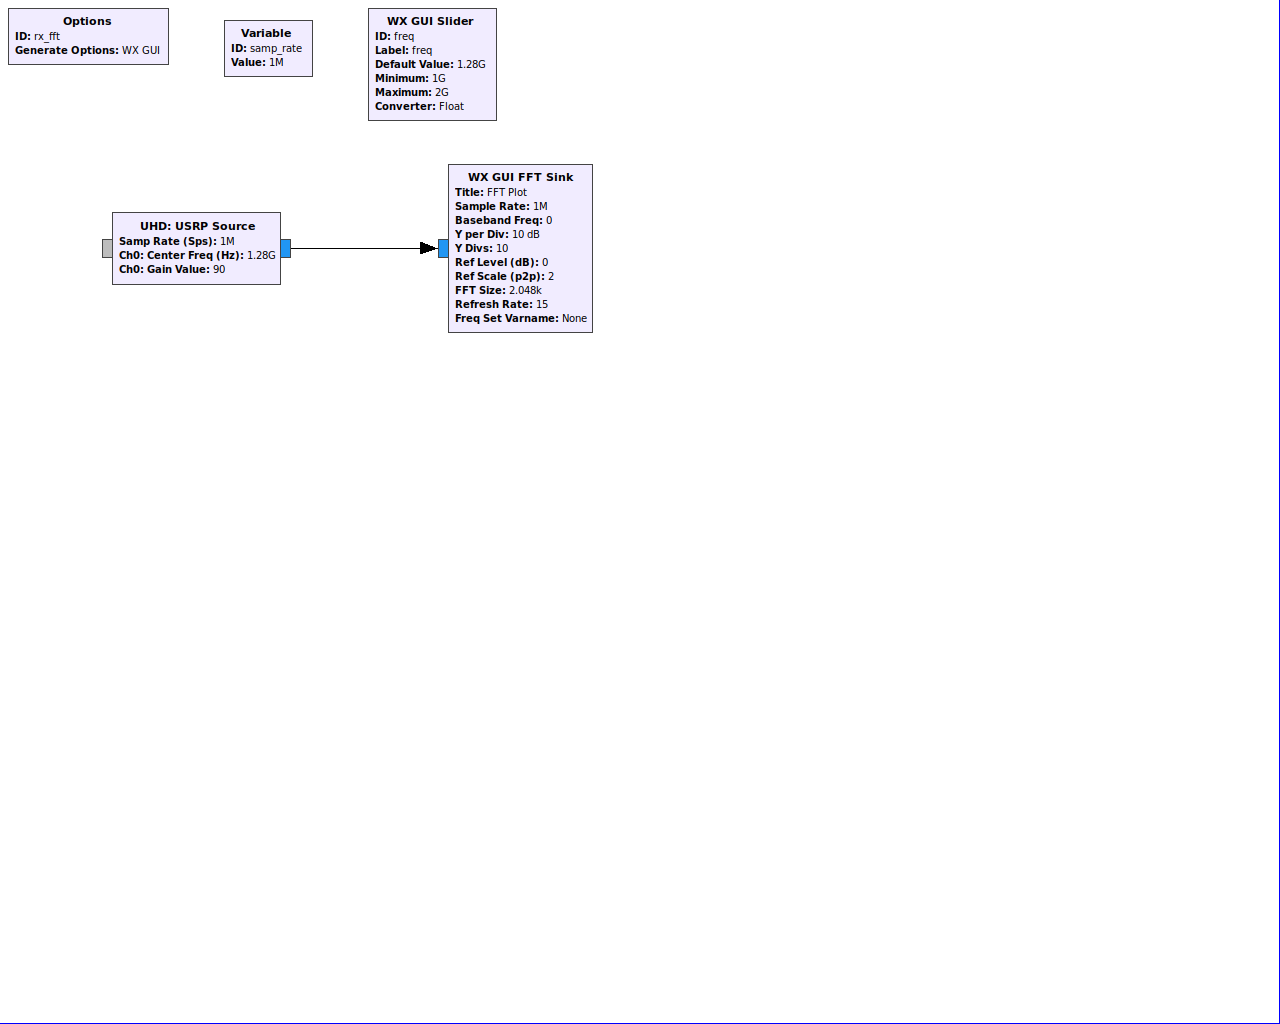
\includegraphics[width=13cm]{figures/dvbt_rx_fft.png}
			\caption{GNU Radio示波器}
			\label{fig:dvbt_rx_fft}
		\end{figure}
		\begin{figure}[htp]
			\centering
			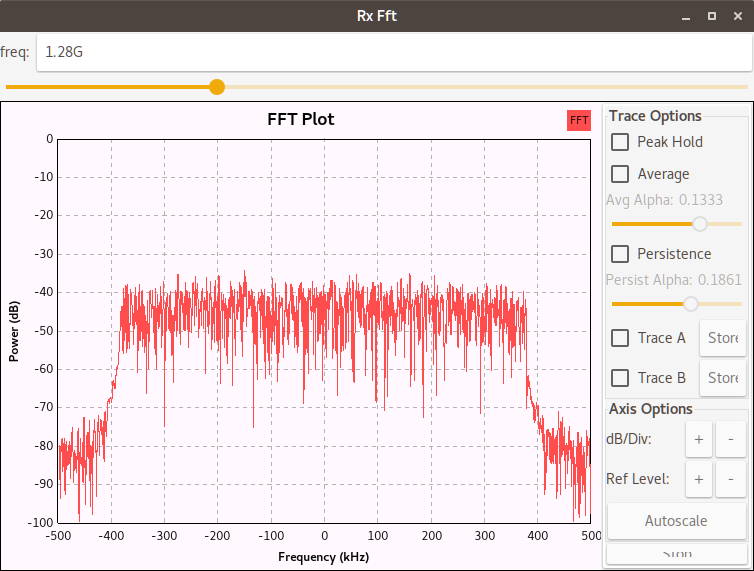
\includegraphics[width=13cm]{figures/dvbt_rx_fft_1.png}
			\caption{GNU Radio示波器}
			\label{fig:dvbt_rx_fft_1}
		\end{figure}
		\par $\bullet$ 使用示波器
		\par 带宽为2MHz时波形如图\ref{fig:dvbt_BW_2MHz}所示,带宽为5MHz时波形如图\ref{fig:dvbt_BW_5MHz}所示。
		\begin{figure}[htp]
			\centering
			\subfigure[带宽为2MHz时示波器波形]{%
				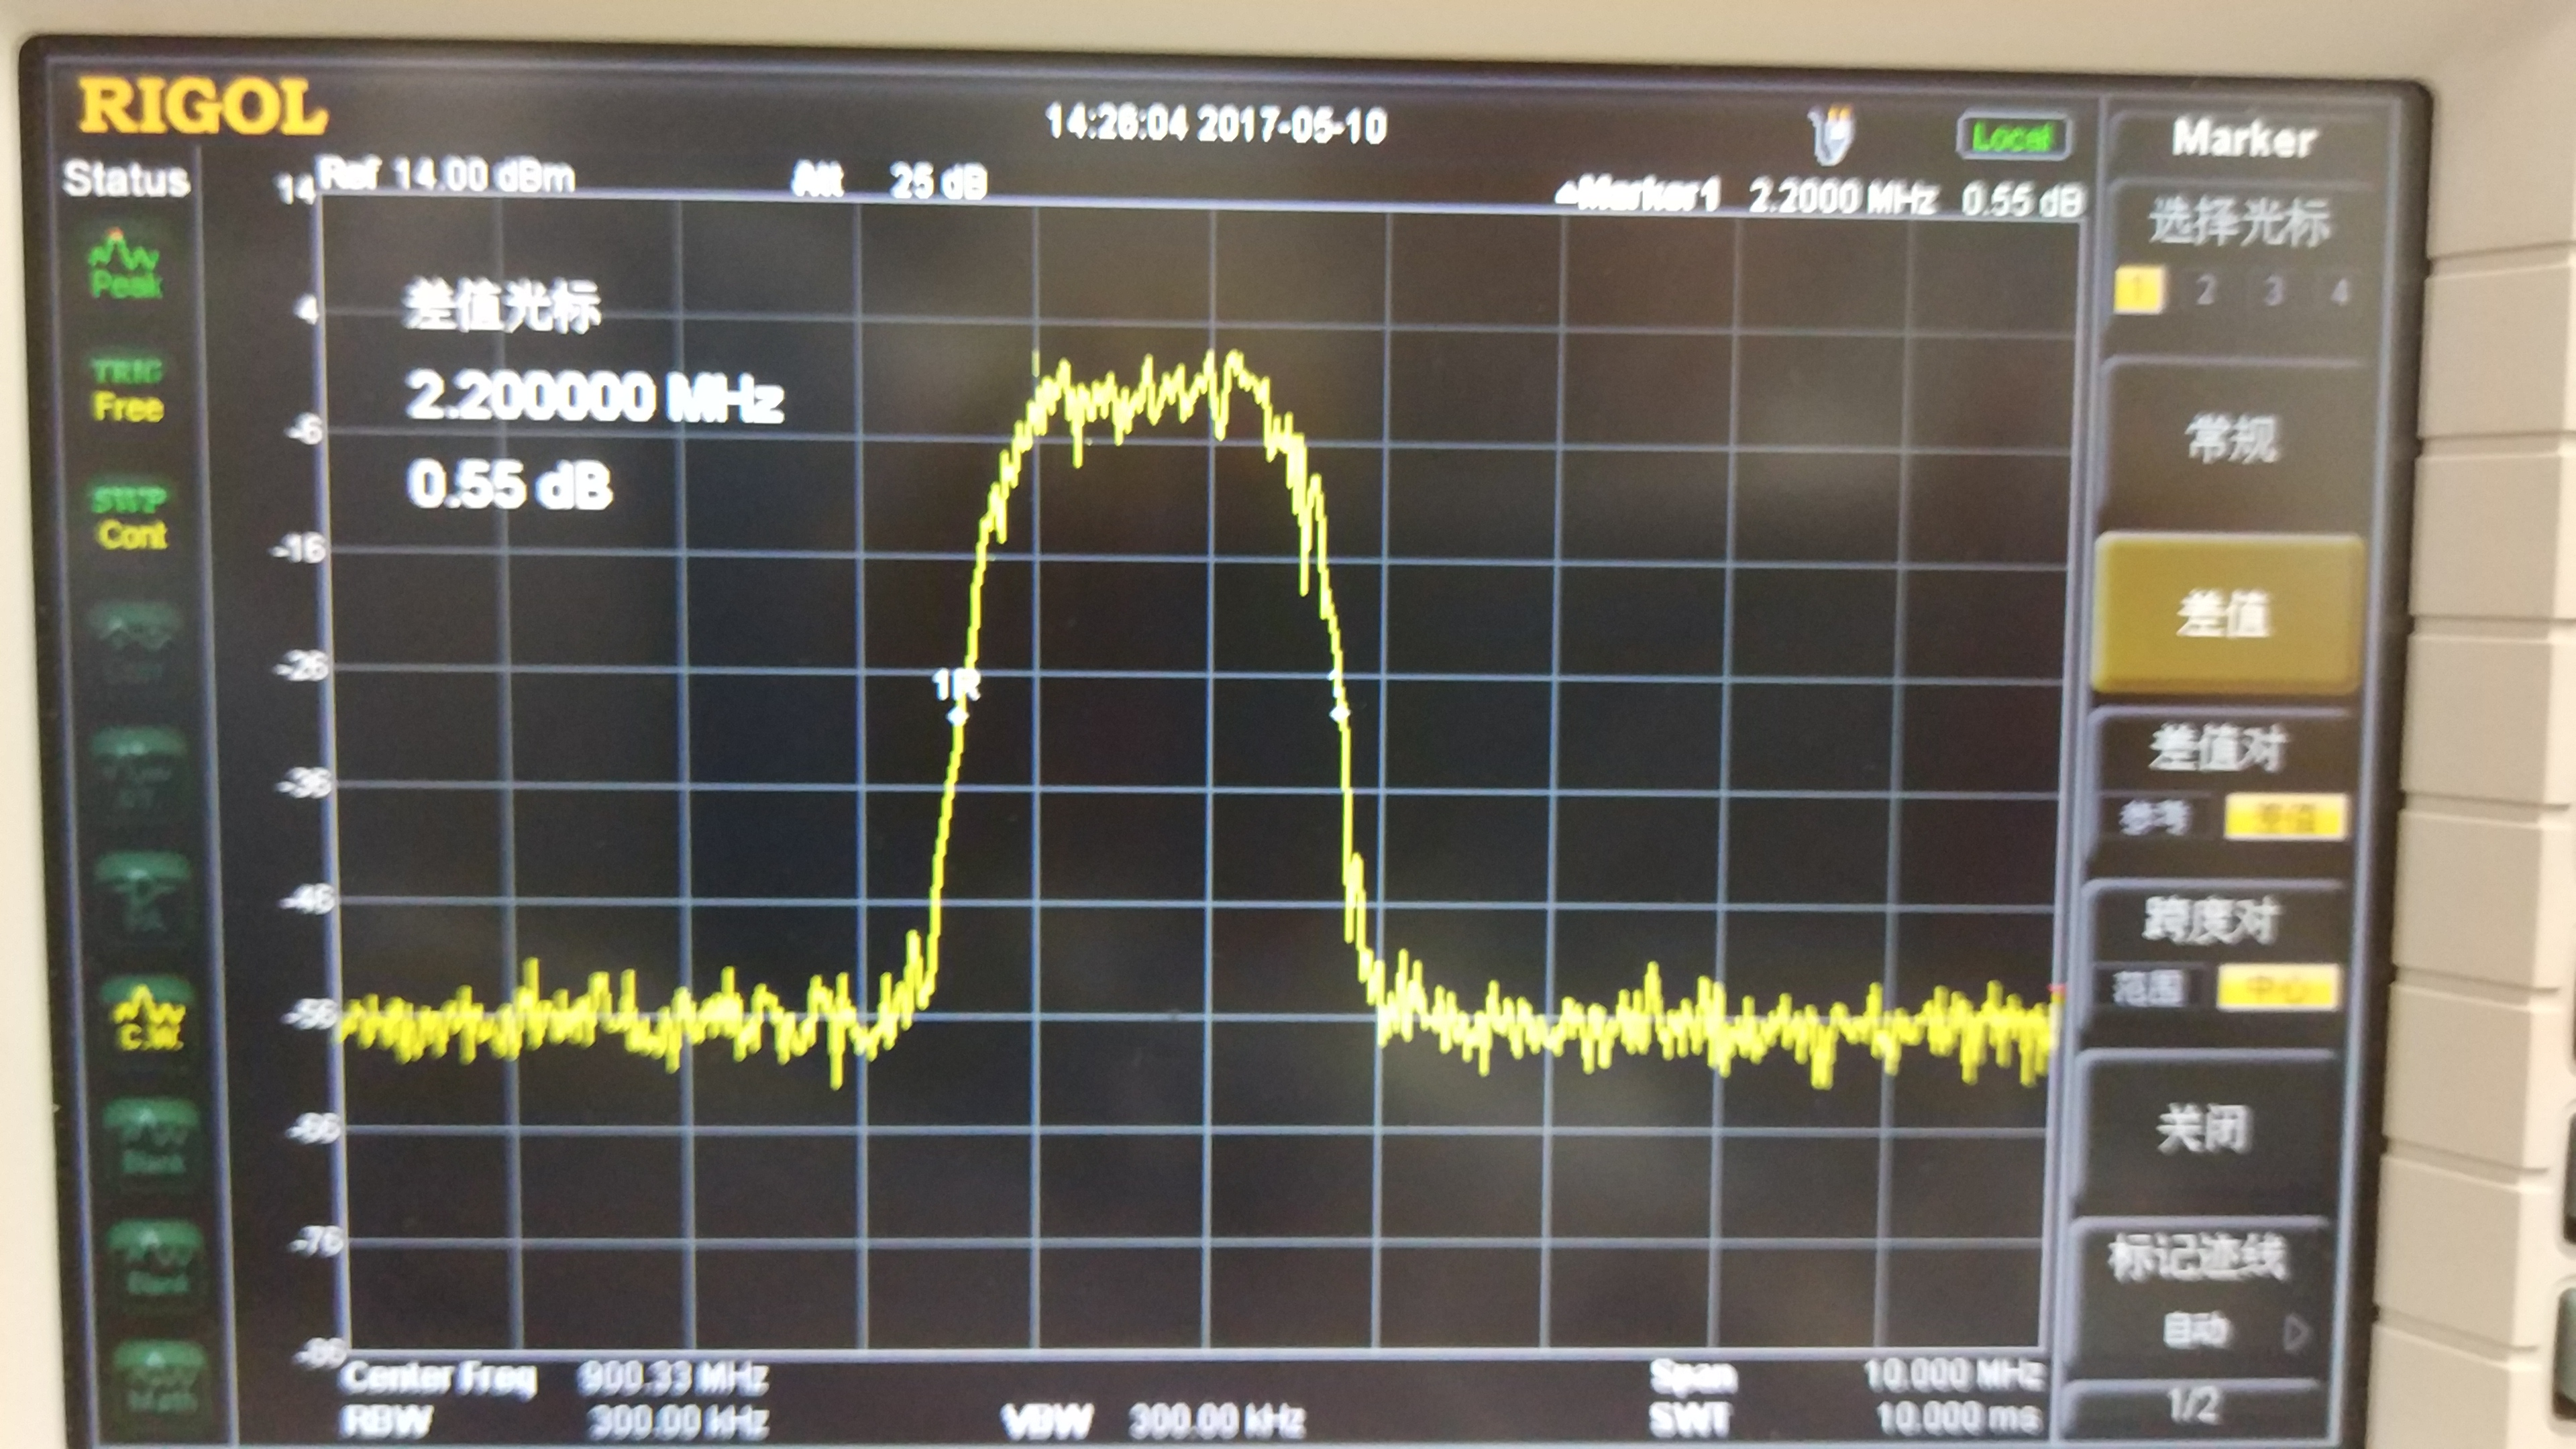
\includegraphics[width=0.4\textwidth]{figures/dvbt_BW_2MHz.jpg}
				\label{fig:dvbt_BW_2MHz}}
			\subfigure[带宽为5MHz时示波器波形]{%
				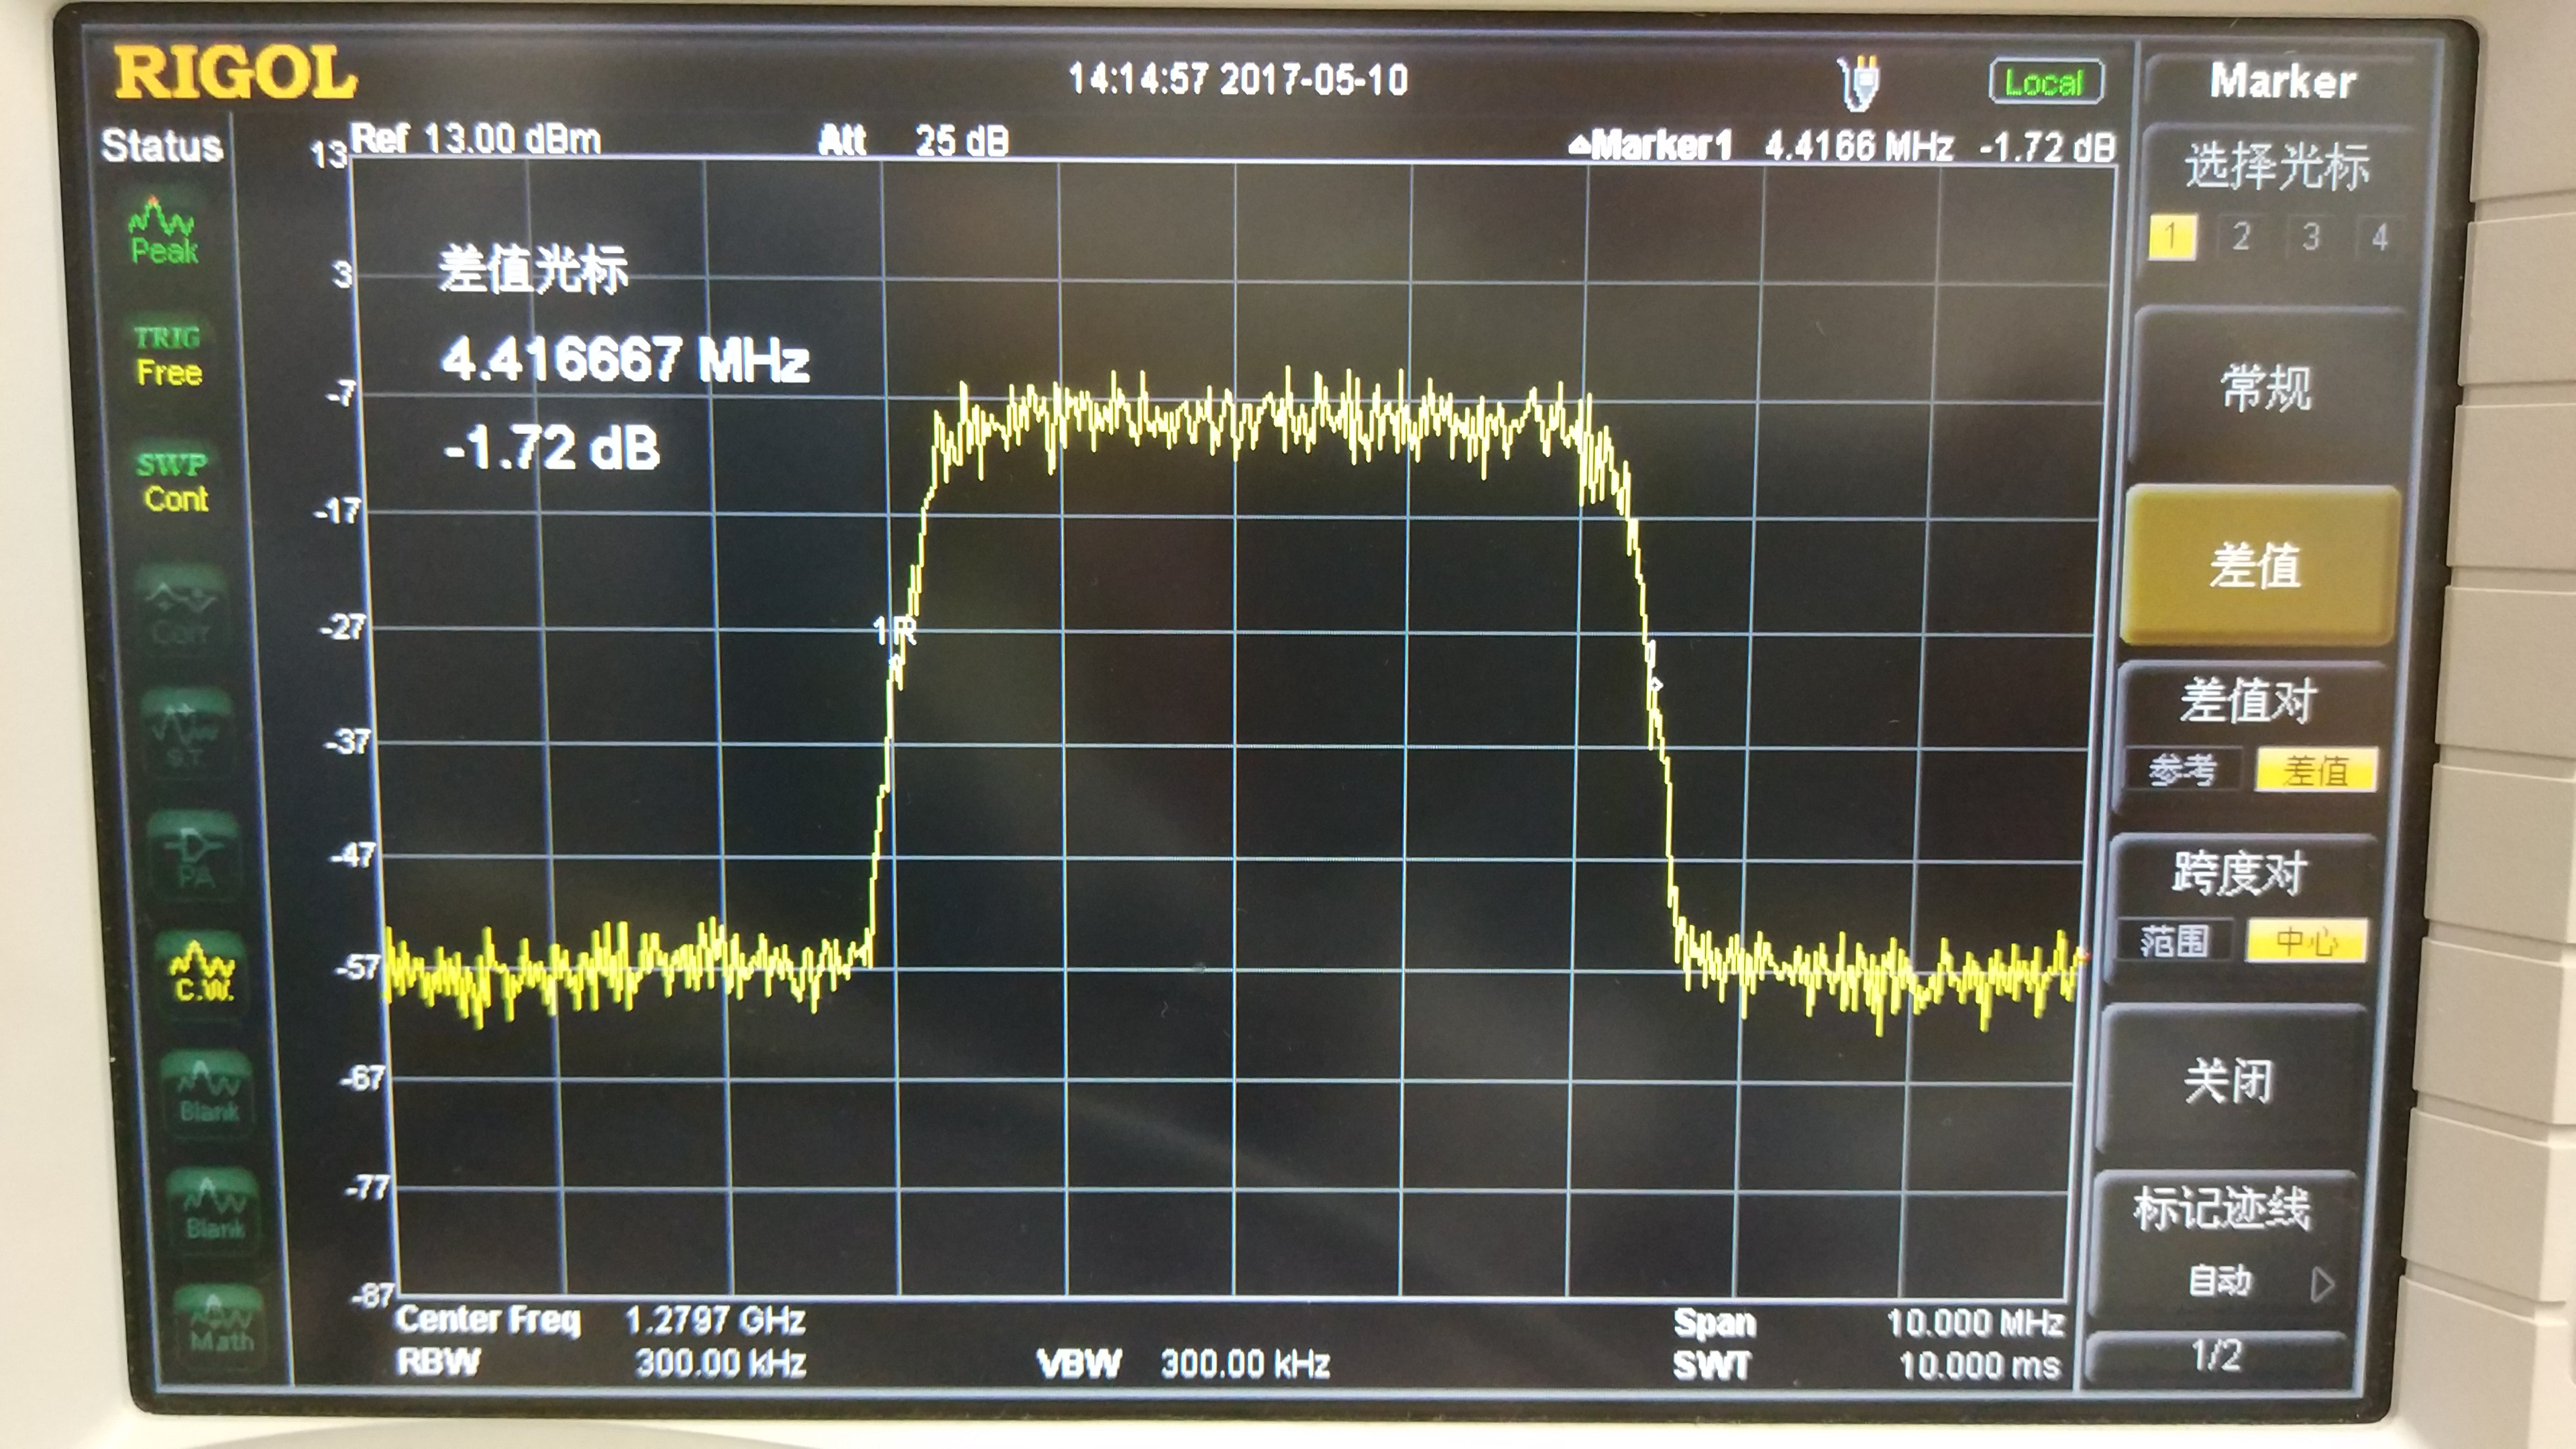
\includegraphics[width=0.4\textwidth]{figures/dvbt_BW_5MHz.jpg}
				\label{fig:dvbt_BW_5MHz}} \\
		\end{figure}
		\par $\bullet$ 使用gqrx
		\par 直接在gqrx中调节到相应频段查看即可,不再赘述。
	\section{距离}
		\par 收发端之间距离较近时可以在当前目录下看到生成的\lstinline[language=sh]{test_out.ts}文件,使用VLC或者Mplayer可以播放出视频,如图\ref{fig:dvbt_rx_TS}。
		\begin{figure}[htp]
			\centering
			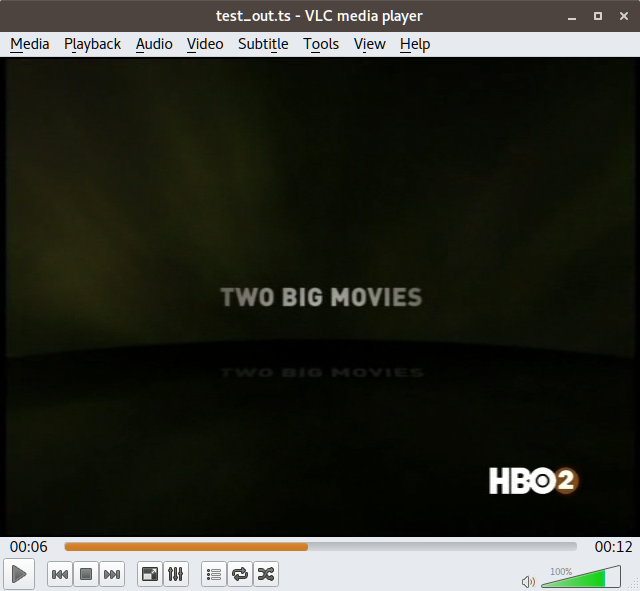
\includegraphics[width=13cm]{figures/dvbt_rx_TS.png}
			\caption{视频输出}
			\label{fig:dvbt_rx_TS}
		\end{figure}
		\par 由于USRP的输出功率,信号能传播大约一间屋子的距离(约5米),超过这段距离将会出现以如图\ref{fig:dvbt_rx_2MHz_ranged_2}无法解星座映射以及如图\ref{fig:dvbt_rx_TS_broken}视频播放失真的情况。
		\begin{figure}[htp]
			\centering
			\subfigure[约5m处星座图]{%
				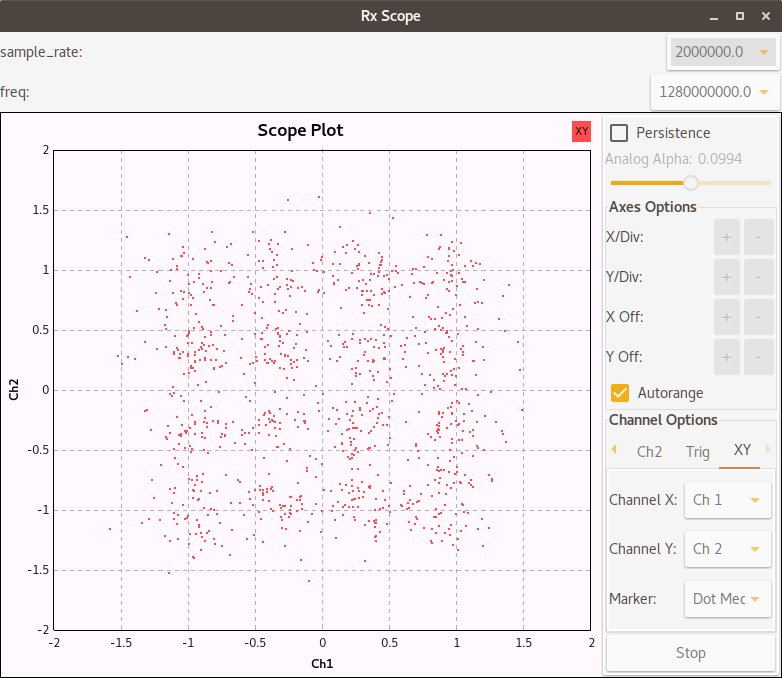
\includegraphics[width=0.4\textwidth]{figures/dvbt_rx_2MHz_ranged_2.png}
				\label{fig:dvbt_rx_2MHz_ranged_2}}
			\subfigure[约5m处视频解码]{%
				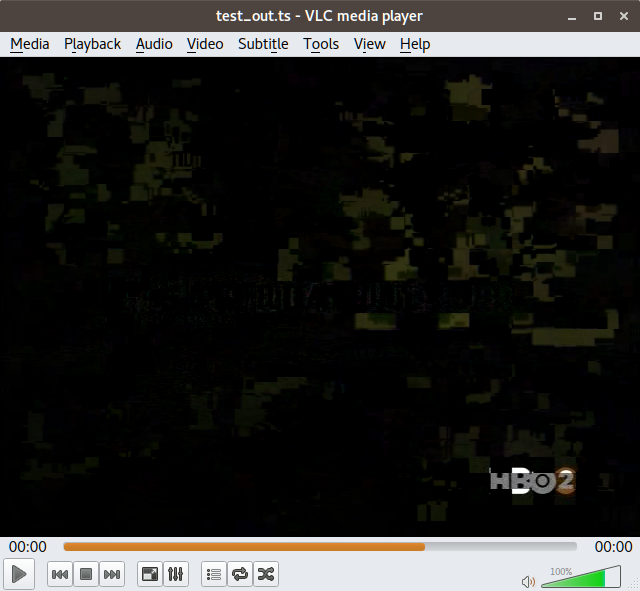
\includegraphics[width=0.4\textwidth]{figures/dvbt_rx_TS_broken.png}
				\label{fig:dvbt_rx_TS_broken}} \\
		\end{figure}
	\section{树莓派发射}
		\par 将设备按图\ref{fig:dvbt_raspi}所示连接,便可以在接收端上看到\lstinline[language=sh]{test_out.ts}但是由于带宽太小,误码率高,在OFDM接收端处无法解码,该文件无法流畅播放。
		\begin{figure}[htp]
			\centering
			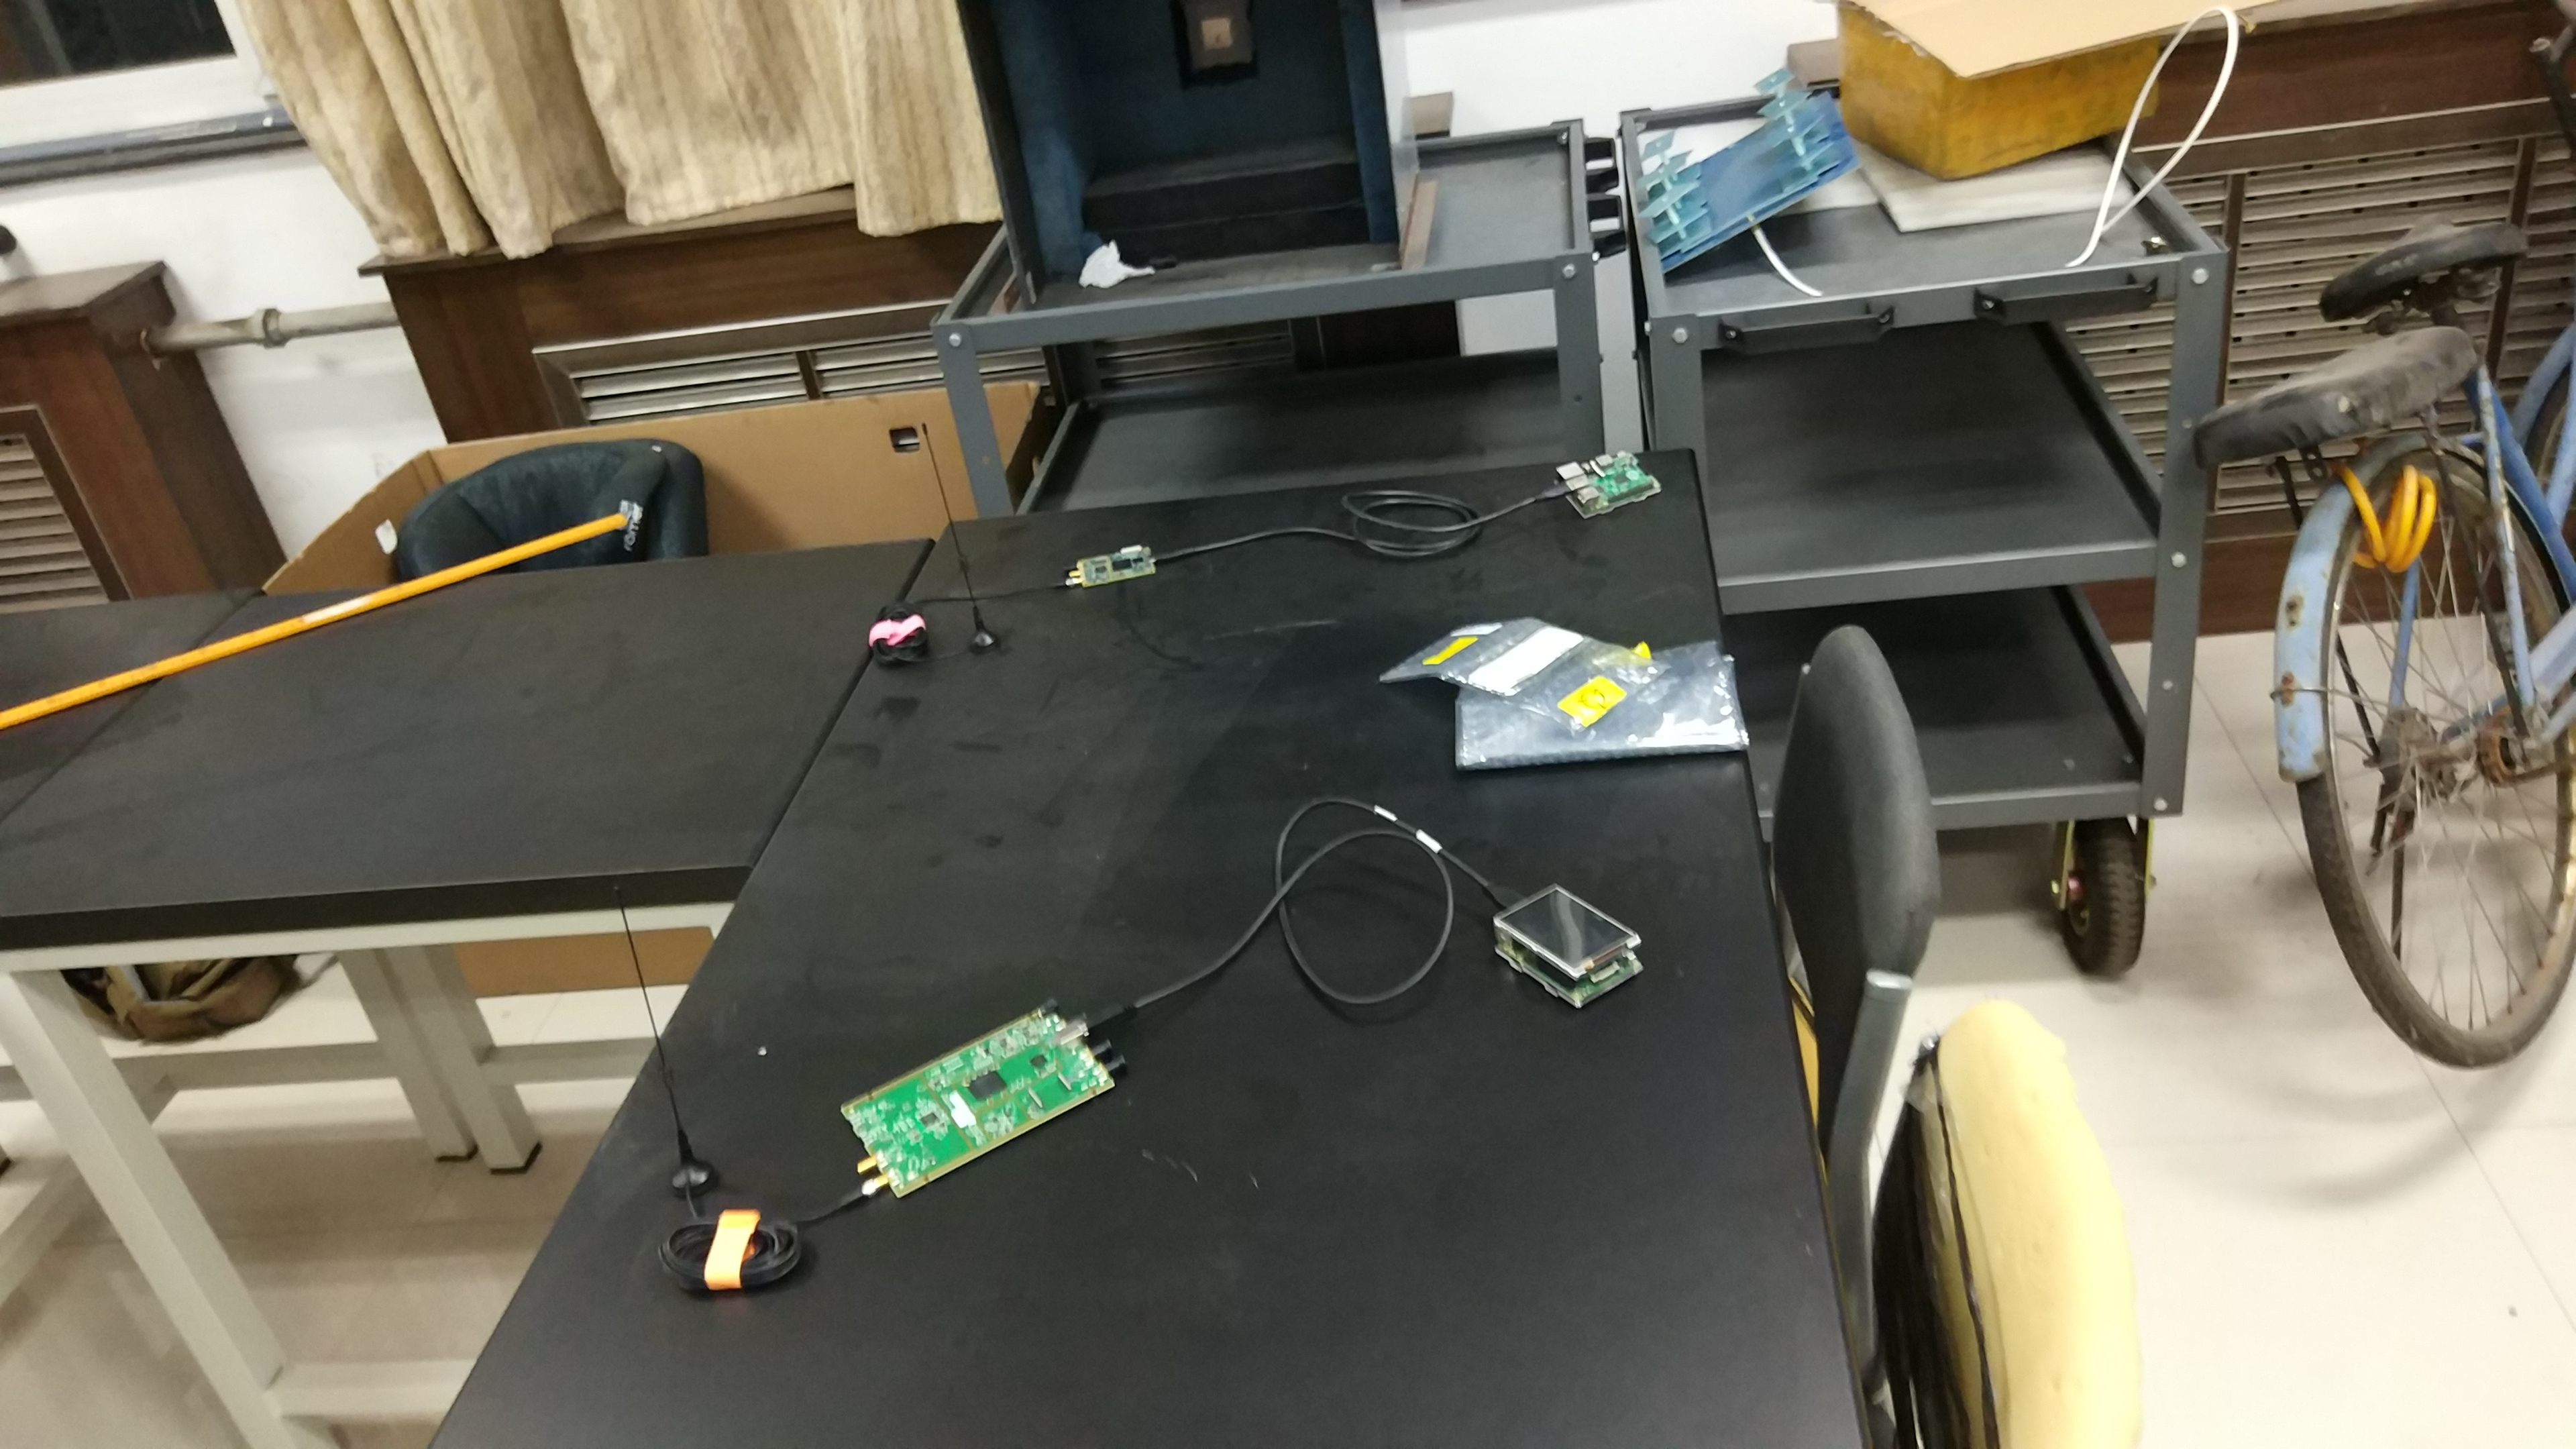
\includegraphics[width=13cm]{figures/dvbt_raspi.jpg}
			\caption{树莓派连接图}
			\label{fig:dvbt_raspi}
		\end{figure}
		\par 由于树莓派的计算性能与IO性能较弱,仅能提供约500KHz的带宽,也许将部分模块交由FPGA处理会有巨大的提升,或者通过gpu来计算相关模块,有待后续开发者继续研究。

%!TEX root = ../paper.tex
\chapter{总结与展望}
	\section{总结}
	\par 本文从树莓派下Linux环境的安装开始,介绍了GNU Radio相关的环境配置,着重介绍了CMake、git和GNU Radio的相关知识,找到了一种在arm架构、低版本GNU Radio下编译gr-dvbt的方法。之后简要介绍了DVB-T的相关知识,介绍了DVB-T发射系统中各个模块的作用,介绍了一些模块的具体实现方法,并给出了一些模块的源码。接下来给出了一个通过GNU Radio搭建一个DVB-T收发系统的框图,该系统能够很好进行MPEG-2 TS视频流的收发,可能由于系统的性能,暂时还没有实现视频的实时收发。在具体实现的后面也给出了该系统的运行效果,包括星座图以及示波器波形,并发现该套系统的最大收发距离约为5米。整个系统在i5-3337U平台上运行时带宽最高可以达到5MHz,搭载在树莓派上时由于系统的处理性能问题,整个系统的带宽仅能达到500KHz,无法完成视频接收端的解码。使用USRP时发现带宽与采样率相同,但并未找到其相同的准确原因,有待更加深入的研究。
	\section{展望}
	\par 本设计通过GNU Radio实现,由于GNU Radio是开源软件,可以通过修改其相关代码来实现一些特殊的功能。可以将相关运算移动到FPGA上来加速运算,因为树莓派提供了一个比较羸弱的GPU,也许可以通过GPU计算FFT来加速整个程序的运行。DVB-T协议对多普勒频移比较敏感,可以采用DVB-H协议来搭建整个系统实现数据信息在移动端的收发。可以修改能量扩散的模块来传递自己需要的格式,并将RS编码等编码方式更换为特定的编码来实现传递其他类型数据信息的系统。由于在开发中因为需要的依赖问题,有可能需要进行频繁的系统重做之类的操作,可以将整个系统放置到Docker上来实现整个系统的版本控制与回溯,从而缩短开发过程。后续开发者可以参考本文来进行快速搭建与修改。
%!TEX root = ../paper.tex
\chapter{致谢}
	\par 大学四年如白驹过隙,在这四年中我获得了身心上的成长,在与各种书本打交道的过程在学习上获得了巨大的成长,在与同学们一起讨论、交流、学习的过程中收获了许许多多的朋友,对我来说,在西工大的这四年是最充实的四年,也是最难忘的四年,这四年将成为这一生中值得回忆的美好记忆。
	\par 经过一学期的努力,我终于完成了毕业设计的制作与毕业论文的编写,在这里特别感谢在写作过程中提供帮助的老师,同学和朋友们。其中,最值得感谢的是李彬老师,是李老师给了我这个课题,提供了相关设备以及思路,并且每周听取汇报为接下来的工作指定目标,使得我能够循序渐进地完成整个毕业设计。在整个毕业设计期间,是李老师在我对各种理论产生困惑时,答疑解惑,提出了众多宝贵的意见,给予了精心的指导,最终使我的毕业论文得以完善。李老师平易近人以及严谨治学的态度使我受益匪浅,在此表示深深的谢意!
	\par 我还要感谢我的父母,感谢他们在我求学路上的默默支持。
	\par 最后,我要郑重的感谢西北工业大学,感谢学校为我提供了优秀的学习氛围,以及对学生的无私栽培。

\sWuhao

% 参考文献设置
\clearpage
\phantomsection
\addcontentsline{toc}{chapter}{\fHei 参考文献}
% npu专用
\bibliographystyle{nputhesis}
% GB专用
% \bibliographystyle{GBT7714-2005NLang}

% 参考文献位置
% \bibliography{references/reference,references/wiki}
\bibliography{references/reference}

\clearpage
\end{document} 